%scrartcl: Für kürzere Ausarbeitungen. Beginnt mit section, es gibt keine chapter
%scrreprt: Für längere Ausarbeitungen (Bacherlo oder Master Thesis). Beginnt chapter
\documentclass[pdftex,a4paper,abstracton,11pt,parskip=half,bibtotocnumbered]{scrartcl} 

% Je nach LaTeX Compiler werden etwas andere Bibliotheken verwendet.
% Das Paket iftex erlaubt es, den Compiler zu überprüfen
\usepackage{iftex}

\usepackage[ngerman]{babel} % Einstellungen für den deutschen Sprachraum, neue deutsche Rechtschreibung
\ifPDFTeX
  \usepackage[utf8]{inputenc} % Umlaute erkennen. Als Option in \glqq [] \glqq  die vom Editor verwendete Zeichencodierung auswählen
  \usepackage[T1]{fontenc}
\fi

% Für kompakter Aufzählungen
\usepackage{paralist}

\usepackage[style=ieee,backend=bibtex]{biblatex}
\addbibresource{literatur/literatur.bib}

% Für Abbildungen
\usepackage{graphicx}
\graphicspath{{./abbildungen/}}

% Ändert die Überschrift des Abstracts.
% Falls kein Abstract benötigt wird, kann die Option \glqq abstracton\grqq{} ganz oben in \documentclass entfallen.
\renewcommand{\abstractname}{Zusammenfassung}

% Für Landscape
\usepackage{pdflscape}
\usepackage{adjustbox}
\usepackage{float}


% Kopfzeile
\usepackage{fancyhdr}
\pagestyle{fancy}
\fancyhead{} % Löscht alle Kopfzeileneinstellungen
\lhead{\leftmark} % Aktuelle Sektion in der linken Kopfzeile
\fancyhfoffset[R]{0cm}

\usepackage[a4paper,left=2.5cm,right=2cm,top=3cm,bottom=2cm,foot=1cm]{geometry}

\title{Neugestaltung von \textit{Schüler Online}: Eine Beobachtungs- und Interviewstudie zur Identifikation von Problemstellen und Nutzerbedürfnissen, um die Effektivität sowie die Zufriedenstellung des Schulpersonals beim Erfüllen von Kernaufgaben der Webanwendung zu optimieren}
\author{Lukas Wessel}
\date{\today}

\begin{document}
\pagenumbering{gobble} % Keine Seitenzahlen bis hier

\makeatletter
\begin{titlepage}
	\centering
	{\scshape\LARGE Fachhochschule Südwestfalen \par}
	\vspace{1cm}
%	{\scshape\Large Merkblatt\par}
	\vspace{1.5cm}
	{\huge\bfseries \@title\par}
	\vspace{3cm}
	{\Large \@author\par}
	\vspace{1cm}
	{\Large \@date\par}
	\vfill

	\raggedright
%	{\large Eingereicht bei:\par}
%	{\large Betreuer 1}
\end{titlepage}
\makeatother

\thispagestyle{empty}
\begin{abstract}
%Ein Abstrakt, also eine Kurzzusammenfassung der Arbeit ist bei einer schriftlichen Ausarbeitung nicht unbedingt notwendig.
%Bei umfangreicheren Arbeiten, also z.~B. einer Bachelor- oder Master-Thesis, sollte die Ausarbeitung in jedem Fall mit einem \textit{Abstract} beginnen.
Offene Punkte, die ich noch erledigen muss:

- Abstract schreiben

- Schüler Online definieren

- Abbildung 1 erläutern, vor allem die Farben

- Bei Abbildung 2 erläutern, wofür die Briefe und Akteure z.B. stehen

- Bilder aus Anhang referenzieren

- Interviews anhängen

- Meister Schüler Modell: Literatur

\end{abstract}

\vfill
\tableofcontents
\pagebreak
\textbf{Gender-Hinweis}

Zur besseren Lesbarkeit wird in dieser Projektarbeit das generische Maskulinum verwendet. Die in dieser Arbeit verwendeten Personenbezeichnungen beziehen sich – sofern nicht anders kenntlich gemacht – auf alle Geschlechter.
\pagebreak

\pagenumbering{arabic} % Beginnt die Seitennummerierung ab hier mit arabischen Zahlen
\setcounter{page}{1}
\title{Neugestaltung von Schüler Online: Eine Beobachtungs- und Interviewstudie zur Identifikation von Problemstellen und Nutzerbedürfnissen, um die Effektivität sowie die Zufriedenstellung des Schulpersonals beim Erfüllen von Kernaufgaben der Webanwendung zu optimieren}

\section{Einleitung}

Das zentrale Anliegen dieser Projektarbeit ist die Untersuchung der Webanwendung "Schüler Online 2.0". Um ein tieferes Verständnis für ihre Funktionalität in der Praxis zu erlangen, werden fünf Sekretärinnen an fünf verschiedenen Schulen mittels eines semistrukturierten Leitfadeninterviews befragt und offen beobachtet. Die Ergebnisse werden im Rahmen dieser Arbeit ausgewertet und analysiert.

Die Relevanz des Themas ergibt sich aus dem Bedarf des Entwicklungsteams, die Verwendungsweise der Anwendung in der Praxis zu verstehen. Trotz vorhandener Forschungen und Literatur über generelle Probleme im Hinblick auf Effektivität und Zufriedenheit sowie über diverse Heuristiken, fehlen spezifische Erkenntnisse für die untersuchte Webanwendung. Die Erforschung dieser Aspekte zielt darauf ab, das System zu optimieren, sodass Schulpersonal Bewerbungen von Schülern effektiv und zufriedenstellend bearbeiten kann. Aspekte der Effizienz sind nicht Gegenstand dieser Studie.

Das Forschungsziel ist es, Einblicke in die Problemstellen zu gewinnen, die das Schulpersonal während des Bewerbungsprozesses eines Schülers hindern könnten, seine Ziele effektiv zu erreichen. Dabei soll untersucht werden, ob die Testpersonen die an sie gestellten Aufgaben mit der Anwendung "Schüler Online 2.0" erfolgreich bewältigen können. 

Die Forschungsmethode umfasst qualitative Auswertungen der Interviews und Beobachtungen, wobei die Testpersonen drei konkrete Aufgaben innerhalb der Anwendung bewältigen sollen. Die Arbeit wird überwiegend induktiv betrieben und versucht, spezifische Erkenntnisse für das untersuchte System zu generieren, um es letztendlich zu verbessern.

Es sei jedoch darauf hingewiesen, dass diese Studie keine konkreten Maßnahmen oder Handlungsanweisungen behandelt. Vielmehr konzentriert sie sich auf die Identifizierung möglicher Problemstellen und Nutzerbedürfnisse, um einen fundierten Ausgangspunkt für zukünftige Forschungen und Entwicklungen zu bieten.

Im Rahmen dieser Studie sollen die folgenden Leitfragen beantwortete werden: 
\begin{itemize}
    \item Wovon handelt Schüler Online, welche Kernaufgaben bildet es ab und welche werden in dieser Studie analysiert? (LF1)% (Theorie)
    \item Wie kann Effektivität im Kontext der Untersuchung definiert werden? (LF2)% (Theorie)
    \item Wie kann Zufriedenheit im Kontext der Untersuchung definiert werden? (LF3)% (Theorie)
    \item Welche typische Problemstellen und Nutzerbedürfnisse gibt es bei Webanwendungen? (LF4)% (Theorie)
    \item Wie sollte so ein Fragebogen aussehen? (LF5)% (Ergebnisteil)
    % \item Welcher Nutzerbedürfnisse gibt es und inwieweit werden sie von der Anwendung erfüllt? (LF7)% (Ergebnisteil)
    \item Welche Problemstellen gibt es bei in Anwendung? (LF6)% (Ergebnisteil)
    \item Erreichen die Nutzer effektiv und zufriedenstellend ihre Ziele? (LF7)% (Diskussion)
\end{itemize}

ALTERNATIV  

Im Rahmen dieser Studie werden mehrere zentrale Fragen untersucht: Zunächst wird die Webanwendung \glqq Schüler Online\glqq  beleuchtet, um zu klären, wovon sie handelt, welche Kernaufgaben sie abbildet, und welche speziell in dieser Studie analysiert werden (LF1). Anschließend wird die Effektivität im Kontext der Untersuchung definiert(LF2), sowie die Zufriedenheit im Kontext der Untersuchung festgelegt(LF3). Die Forschung zitiert typische Problemstellen und Nutzerbedürfnisse bei Webanwendungen(LF4). Zudem wird erörtert, wie ein entsprechender Fragebogen aussehen sollte, um die benötigten Daten zu sammeln (LF5). Weiterhin wird untersucht, welche Problemstellen bei der Anwendung konkret aufgetreten sind (LF6), und abschließend bewertet, ob die Nutzer effektiv und zufriedenstellend ihre Ziele erreichen (LF7).

\pagebreak
%Das Thema dieser Projektarbeit behandelt die Webanwendung textit{Schüler Online 2.0}. Hierzu %werden bei insgesamt fünf Sekretärinnen an fünf verschiedenen Schulen ein semistrukturiertes %Leitfadeninterview durchgeführt und die Testpersonen offen beobachtet, und im Rahmen dieser %Projektarbeit ausgewertet.
%
%Das Thema ist relevant, da dem Entwicklungsteam bislang keine Klarheit darüber vorliegt, wie %die Anwendung in der Praxis performt.
%Die Forschung wird überwiegend induktiv betrieben, es gibt zwar in der Literatur bereits %Erkenntnisse darüber, welche Probleme hinsichtlich Effektivät und Zufriedenstellung sowie %diverse Heuristiken, nicht allerdings speziell für die zu untersuchende Webanwendung. Ebendas %soll untersucht werden, damit die Anwender die Bewerbungen von Schülern effektiv und %zufriedenstellend erfassen und bearbeiten können.
%
%Das Ziel der Forschung ist es, einen Einblick zu gewinnen, welche Problemstellen und %Nutzerbedürfnisse das Schulpersonal beim Bewerbungsprozess eines Schülers und den Nutzer daran %hindern, sein Ziel effektiv und zufriedenstellend zu erreichen. Es soll herausgefunden werden, %ob die Testpersonen die Aufgabenstellungen effektiv und zufriedenstellend erledigen können. Die %Ergebnisse der Interviews und Beobachtungen werden hierfür qualitativ ausgewertet. Die %Forschung wird betrieben, indem Personen aus der genannten Gruppe drei Aufgaben in der %Anwendung Schüler Online bewältigen sollen. 




%Zu Beginn der Ausarbeitung ist es besonders wichtig, dem Leser zu erklären, warum Sie das Thema bearbeiten.
%Dabei ist nicht unbedingt Ihre eigene Motivation gemeint, sondern vielmehr die Frage, warum die Problemstellung Ihrer Arbeit relevant ist.
%Angemessene Motivationsgründe sind etwa:
%\begin{compactitem}
%\item Sie lösen ein Problem, für das es bisher keine, oder keine gute Lösung gibt.
%\item Ein Unternehmen kann Ihre Lösung einsetzen, um damit Profit zu erwirtschaften.
%\item Sie vergleichen verschiedene Produkte oder Methoden, um damit die Entscheidungsfindung bei der Auswahl zu erleichtern.
%\item Sie stellen ein komplexes Thema für eine bestimmte Zielgruppe angemessen dar.
%\end{compactitem}
Die zugrunde liegende Problemstellung ist relevant für den Hersteller der Anwendung \glqq Schüler Online"(\glqq Kommunales Rechenzentrum Minden/Ravensberg-Lippe"), da Unklarheit herrscht, ob die Anwender die Software korrekt bedienen können. Die Korrektheit ist auch für die Anwender wichtig, da die Anwendung das Schulgesetz abbilden soll und eine korrekten Erfüllung ermöglichen soll. Der Nutzer der Anwendung soll zufrieden sein, seine Erwartungen und Bedürfnisse an die Software sollen erfüllt werden. Mit der vorliegenden Studie soll geprüft werden, inwieweit die Software ebenjenen entspricht oder abweicht.

Es gibt zwar bereits Forschungen hinsichtlich häufig vorkommenden Problemstellen und Nutzerbedürfnissen von diversen Autoren, 
%wie bspw. 
allerdings liegt noch keine Forschung zur Webanwendung \glqq Schüler Online" im Bereich des Usability Engineerings vor. 

\section{Theoretischer Hintergrund}
\subsection{Die Webanwendung \textit{Schüler Online}}
Schüler Online ist eine Webapplikation, die die Anmeldung von Schülern an Schulen erleichtert. Die primär involvierten Parteien umfassen Schüler, Eltern und Schulen. Die Schulen bearbeiten hauptsächlich die Anmeldungen und entscheiden über Aufnahmen. Kreise und Gemeinden sind ebenfalls beteiligt, sie lesen Statistiken und kontrollieren die Schulpflicht. Ausbildungsbetriebe und Administratoren spielen auch eine Rolle; die Betriebe agieren als Partner für Ausbildungen, und die Administratoren pflegen die Stammdaten. Anmeldungen können von Schülern, Eltern, Schulen, Gemeinden oder Betrieben erstellt und modifiziert werden. Diese Ausarbeitung konzentriert sich auf den Prozess, bei dem Schulen selbst die Anmeldungen anlegen und die eingegangenen Anmeldungen bearbeiten.\cite{ProductOwner2023}

\subsection{Definition von Effektivität im Rahmen dieser Ausarbeitung }
Die ISO 9241-110 definiert Effektivität wie folgt: \glqq Effektivität = Die Genauigkeit und Vollständigkeit mit der Benutzer ein bestimmtes Ziel erreichen.\grqq{}\cite{ISO-9241-110}
In Anlehnung an diese Definition kann festgelegt werden, dass Effektivität im Sinne dieser Ausarbeitung das Ausmaß der Genauigkeit und Vollständigkeit mit dem die Studienteilnehmer die drei an sie gestellten Aufgaben erreichen. 

Erfolgskriterien, die darauf hinweisen, dass eine Aufgabe erfolgreich abgeschlossen wurde, sind: 
\begin{itemize}
    \item Die Navigation zur Aufgabe wurde erfolgreich abgeschlossen (EK1)
    \item Die Pflichtangaben wurden vollständig erfasst (EK2)
    \item Der Aufnahmestatus ist entweder \textit{Aufgenommen}, \textit{Abgelehnt} oder \textit{Warteliste} (EK3)
    \item Die Anmeldung wurde erfolgreich gespeichert (EK4)
\end{itemize}

\subsection{Definition von Zufriedenstellung im Rahmen dieser Ausarbeitung}
Die ISO 9241-110 definiert Zufriedenstellung: \glqq Das Ausmaß der Übereinstimmung der physischen, kognitiven und emotionalen Reaktionen des Benutzers, die aus der Benutzung eines Systems, eines Produkts oder einer Dienstleistung resultieren, mit den Benutzererfordernissen und Benutzererwartungen.\grqq{}\cite{ISO-9241-110} Hieran anknüpfend kann man für die vorliegende Studie festlegen, dass Zufriedenstellung das Ausmaß der Übereinstimmung zwischen den aus der Benutzung von \textit{Schüler Online} entstandenen Reaktionen des Schulpersonals und den Benutzererfordernissen und Benutzererwartungen ist. 

\subsection{Definition von Problemstellen im Rahmen dieser Ausarbeitung}
Im Rahmen dieser Arbeit bezieht sich der Begriff \textit{Problemstelle} auf spezifische Elemente der \textit{Schüler Online}-Anwendung, die bei ihrer Nutzung durch das Schulpersonal zu Defiziten in Bezug auf Effektivität und Zufriedenheit führen.

\subsection{Definition von Nutzerbedürfnissen im Rahmen dieser Ausarbeitung}
Stangl beschreibt den Begriff \textit{Bedürfnis} als \glqq das Verlangen oder der Wunsch, einen empfundenen oder tatsächlichen Mangel Abhilfe zu schaffen.\grqq{}\cite{stangl-beduerfnis} Dies wirft die Frage auf, was ein Mangel im Kontext einer Anmeldung an einer Schule für den Anwender bedeutet. Wenn man herkömmliche Anmeldungen mittels eines Papierformulars betrachtet, kann man hier argumentieren, dass mehrere Aspekte mangelhaft sind. Beispielsweise gibt es keine Validierung der Daten hinsichtlich Korrektheit oder Plausibilität.  Datenvalidierung könnte allerdings durch eine gute Kommunikation mit der abgebenden Schule abgesichert werden. Das Einlesen der Daten ist möglicherweise problematisch, da handschriftliches Ausfüllen unleserlich geschrieben sein kann. Eine Übertragung in verwendete Schulsoftware, wie \textit{SchILD}\footnote{SchILD ist eine so genannte Schulverwaltungssoftware, mit denen die Sekretariate die Schülerdaten ihrer aktuell an der Schule studierenden Schüler administrieren.} kann nur durch unkomfortables Abtippen erreicht werden.
Eine auf diesen Argumenten basierende modellhafte Definition im Kontext dieser Arbeit kann also lauten: \glqq Nutzerbedürfnisse ist das Verlangen oder der Wunsch, die Datenerfassung der Anmeldung weder unsicher, inkorrekt, unplausibel noch unkomfortabel zu vollziehen\grqq{}.

%\begin{itemize}
%    \item \textbf{Schlechte Navigationsstrukturen:} Wenn Nutzer Schwierigkeiten haben, sich auf einer Website zurechtzufinden, können sie ihre Ziele nicht effektiv erreichen. Eine klare, konsistente und intuitive Navigationsstruktur ist entscheidend.
%    \item \textbf{Nicht erfüllte Erwartungen:} Wenn das Design oder die Funktionalität der Anwendung nicht den Erwartungen der Nutzer entspricht, können diese ihre Ziele nicht effektiv erreichen. Beispielsweise kann eine Schaltfläche, die aussieht, als würde sie eine bestimmte Aktion auslösen, tatsächlich eine ganz andere Aktion auslösen.
%    \item \textbf{Mangel an Feedback:} Nutzer müssen wissen, was passiert, wenn sie eine Aktion ausführen. Wenn eine Anwendung nicht angemessen auf Nutzereingaben reagiert, kann dies zu Frustration und Ineffektivität führen.
%    \item \textbf{Nicht zugängliches Design:} Webanwendungen sollten für alle Benutzer, einschließlich Menschen mit Behinderungen, nutzbar sein. Eine Anwendung, die nicht die Richtlinien für Barrierefreiheit erfüllt, kann für einige Nutzer ineffektiv sein.
%    \item \textbf{Schlechte Leistung:} Langsame Ladezeiten oder technische Probleme können die Effektivität stark beeinträchtigen, da sie Nutzer daran hindern, ihre Ziele in einer angemessenen Zeit zu erreichen.
%    \item \textbf{Komplizierte oder überladene Benutzeroberflächen:} Wenn eine Benutzeroberfläche zu viele Optionen, zu viel Text oder zu viele Bilder enthält, kann dies Benutzer verwirren und ihre Fähigkeit, ihre Ziele effektiv zu erreichen, beeinträchtigen.
%    \item \textbf{Mangel an Suchfunktion oder ineffektive Suchfunktionen:} Eine effektive Suche ist für viele Webanwendungen entscheidend. Wenn Nutzer nicht finden können, was sie suchen, können sie ihre Ziele nicht effektiv erreichen.
%
%    %Bedienfehler
%    %Entspricht Gewohnten Abläufen
%    %Nimmt Arbeit ab
%    %Schwierige Bedienung
%    %Suchen nach: \glqq Common usability problems in web applications\grqq{} 
%\end{itemize}

%evtl. wie sieht das schulgesetz aus oder der Prozess


\section{Material und Methode}
\subsection{Teilnehmerauswahl}

In der vorliegenden wissenschaftlichen Arbeit wurde auf zwei divergierende Pools zur Rekrutierung der Teilnehmer zurückgegriffen. Der erste Rekrutierungspool umfasste diejenigen Individuen oder vermittelnden Kontakte\footnote{Ein vermittelnder Kontakt ist ein Kontakt, der einen potenziellen Studienteilnehmer aus seinem persönlichen Umfeld kontaktiert hat und diesen gefragt hat, ob er an der Studie teilnehmen möchte}, die eine Schulung für \textit{Schüler Online} besucht hatten. In diesen Schulungen wurde am Ende eine Folie präsentiert, die diese Studie vorstellte und um die Beteiligung der Anwesenden bat. Aus diesem Pool wurde die Sekretärin des Berufskollegs akquiriert.

Ein alternativer Weg zur Gewinnung von Teilnehmern war die Kaltakquise. Aus diesem Pool kamen alle weiteren Teilnehmer. Dabei wurden Schulen in zwei umliegenden Kreisen telefonisch kontaktiert und um ihre Teilnahme an der Studie gebeten. Aus Gründen der Vertraulichkeit und der Einhaltung von Verschwiegenheitsvereinbarungen ist es an dieser Stelle nicht möglich, konkrete Angaben zur Region zu machen.

Die Auswahl der Teilnehmer erfolgte basierend auf einer Reihe von Kriterien. Wesentlich war, dass die Teilnehmer in ihrem beruflichen Alltag das zu untersuchende Produkt sinnvoll einsetzen konnten - dies war ein entscheidendes Inklusionskriterium. Besonders geeignet waren daher Sekretariatsmitarbeiter, Schulverwaltungsassistenten und potenziell auch Schulleitungen. Als weiteres Inklusionskriterium war es erforderlich, dass die Teilnehmer aktiv in den genannten Berufen tätig und nicht in den Ruhestand getreten waren.

Im Gegenzug dazu wurden Auszubildende und Referendare von der Studie ausgeschlossen, da sie nur begrenzte Erfahrungen mit dem Tätigkeitsfeld der Software hatten. Dies stellte ein explizites Exklusionskriterium dar. Darüber hinaus spielten Faktoren wie Alter, Geschlecht, Berufserfahrung, ethnischer Hintergrund und sozioökonomischer Status der Teilnehmer bei der Rekrutierung keine Rolle.

Die Teilnahme an der Studie erforderte nur die Verfügbarkeit und die Bereitschaft der Teilnehmer, sich freiwillig zu engagieren. Es wurde darauf geachtet, dass keine Teilnahmeverpflichtungen, beispielsweise durch Vorgesetzte wie der Schulleitung, entstanden.

\subsection{Umgebungsbedingungen der Beobachtungen und Interviews}

Die Beobachtungen und Interviews wurden im Rahmen eines Feldtests abgehalten und fanden während der regulären Arbeitszeit an den gewohnten Arbeitsplätzen der Studienteilnehmer statt, um realistische Szenarien zu erzeugen. 

Die Durchführung der Interviews wurde während der Sommerferien terminiert. Es war von Bedeutung, den tatsächlichen Arbeitskontext der Teilnehmer einzubeziehen, um ein möglichst repräsentatives Bild ihrer Erfahrungen und Herausforderungen im Umgang mit dem untersuchten Produkt zu gewinnen.

\subsection{Erstellung des Fragebogens}

Die Formulierung des Fragebogens erfolgte durch eine Expertengruppe, die aufgrund ihrer beruflichen Rolle und Erfahrung eine hohe fachliche Expertise in Bezug auf die Anforderungen der zu untersuchenden Software besaßen. Diese Gruppe setzte sich zusammen aus Individuen, die im beruflichen Kontext die Anforderungen an die Software definierten und dokumentierten. Innerhalb dieser Gruppe gab es keinen Usability Experten, ledigliche einen Studenten, der das Fach \glqq Usability Engineering\grqq{} in seinem Studium belegte.

Um die Qualität und Eignung des Fragebogens zu gewährleisten, wurde dieser nach der Erstellung von einem Experten für Usability Engineering überprüft und auf seine inhaltliche Eignung hin bewertet.

Die Formulierung der Fragen folgte bestimmten Richtlinien: Sie sollten klar und verständlich sein und offen formuliert werden, um eine breite Palette von Antworten zu ermöglichen. Es war hier wichtig, dass der verwendete Sprachschatz laut Kruse den Kenntnissen eines Mitarbeitenden im Schulsekretariat entspricht.\cite{Kruse_2015} Dies gewährleistete, dass alle Teilnehmer die Fragen ohne zusätzliche Erläuterungen verstehen und beantworten können.

\subsection{Entwicklung von Aufgaben und Szenarien}
\begin{figure}[H]
    \caption{Einordnung der Aufgaben in den Gesamtkontext der Anwendung im Rahmen einer Beobachtungs- und Interviewstudie zur Bestimmung der Effektivität und Zufriedenstellung}
    \label{fig:EinordnungAufgaben}
    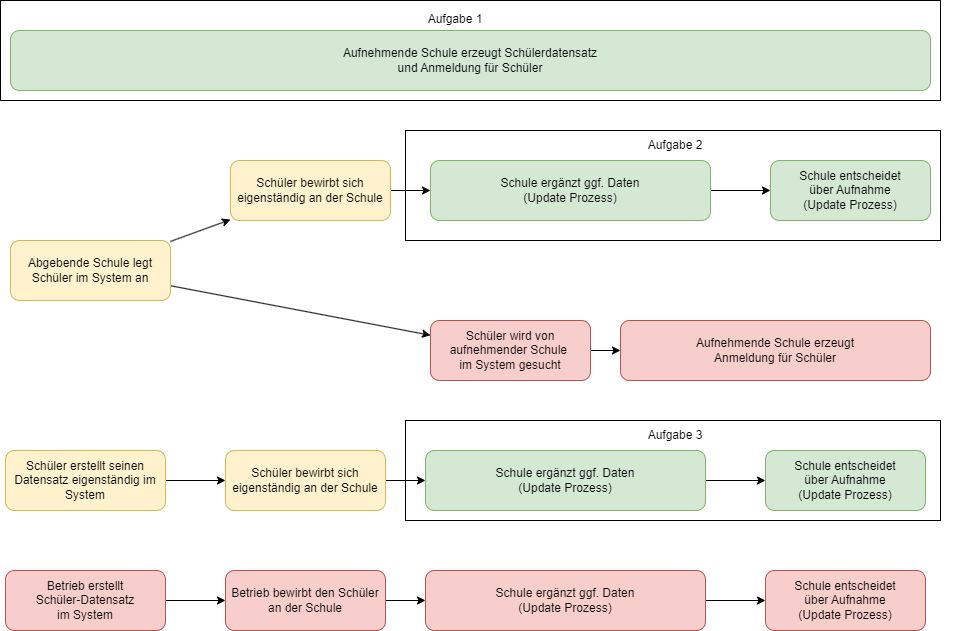
\includegraphics[width=\textwidth]{einordnung-der-aufgaben-in-kontext}
\end{figure}

Für die Durchführung des Feldtests wurden drei spezifische Aufgaben im System entwickelt, die die Teilnehmer während ihrer normalen Arbeitszeit bewältigen sollten. Dabei wurde darauf geachtet, dass die individuellen  Voraussetzungen für die jeweilige Schule gegeben waren, einschließlich  vorhandener Bildungsangebote an der jeweiligen Schule. Die konkreten Aufgaben lauteten wie folgt:

\begin{itemize}
\item Aufgabe 1: \glqq Erstellen Sie bitte für dieses Anmeldeformular von \textit{Max Müller} eine Bewerbung an Ihrer Schule.\grqq{} (Ein Musterexemplar eines solchen Formulars ist Anhang 1 zu entnehmen. Aufgabe 1 macht bisher rund 3,6\% aller erfassten Anmeldungen aus)
\item Aufgabe 2: \glqq Bearbeiten Sie bitte die Bewerbung von \textit{Lotta Meier} nach eigenem Ermessen.\grqq{}  Dieser fiktive Datensatz war so gestaltet, dass die Bewerbung entweder von einer abgebenden Schule oder von der Gemeinde gestellt wurde. Aufgabe 2 macht bisher rund 49,2\% aller erfassten Anmeldungen aus.
\item Aufgabe 3: \glqq Bearbeiten Sie bitte die Bewerbung von \textit{Konrad Schulz} nach eigenem Ermessen.\grqq{}  Bei diesem fiktiven Datensatz wurde die Bewerbung von den Eltern des Schülers eingereicht. Aufgabe 3 macht bisher rund 23,3\% aller erfassten Anmeldungen aus.\footnote{Die Datenquelle der Anteile sind interne Auswertungen des krz.}
\end{itemize}

Andere Anmeldearten sind nicht Gegenstand dieser Untersuchung, da sie zu umfangreich nachzustellen wären. Eine Visualisierung der drei Aufgaben inklusive ihres Kontextes sind in Abbildung \ref{fig:EinordnungAufgaben} ersichtlich. Die rot markierten Aktivitäten werden nicht untersucht. Gelb Markiertes sind vorbereitete Aktivitäten, welche Voraussetzung für die grün markierten zu untersuchenden Aufgabenaktivitäten sind. 

\begin{figure}[H]
    \caption{Übersicht der Aufgabenkonstellationen, gruppiert nach Schulstufe im Rahmen einer Beobachtungs- und Interviewstudie zur Bestimmung der Effektivität und Zufriedenstellung}
    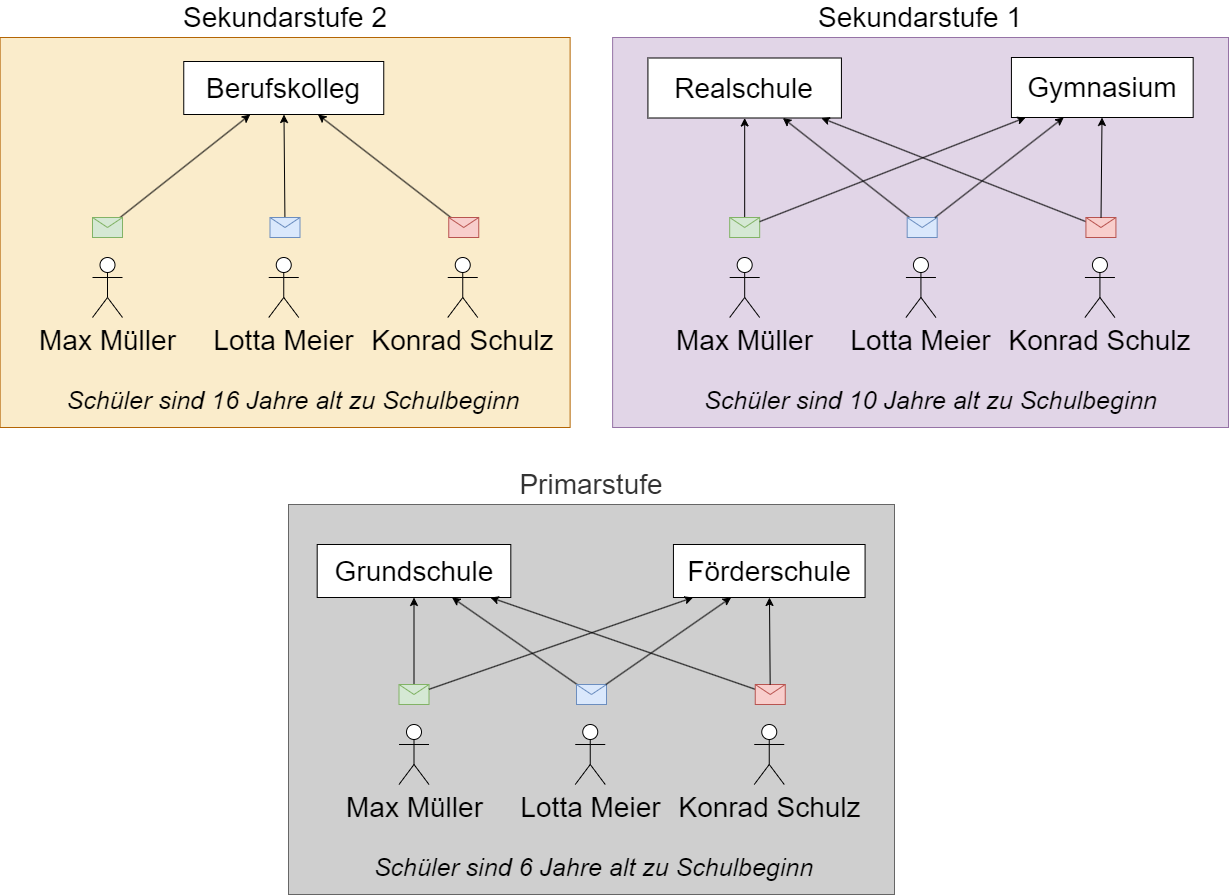
\includegraphics[width=\textwidth]{konstellationenv3}
    \label{fig:konstellationenv3}
\end{figure}

%\begin{figure}[H]
    %\centering
    %\caption{Musteranmeldeformular von der fiktiven Person Max Müller}
    %\begin{adjustbox}{width=\linewidth, center}
        %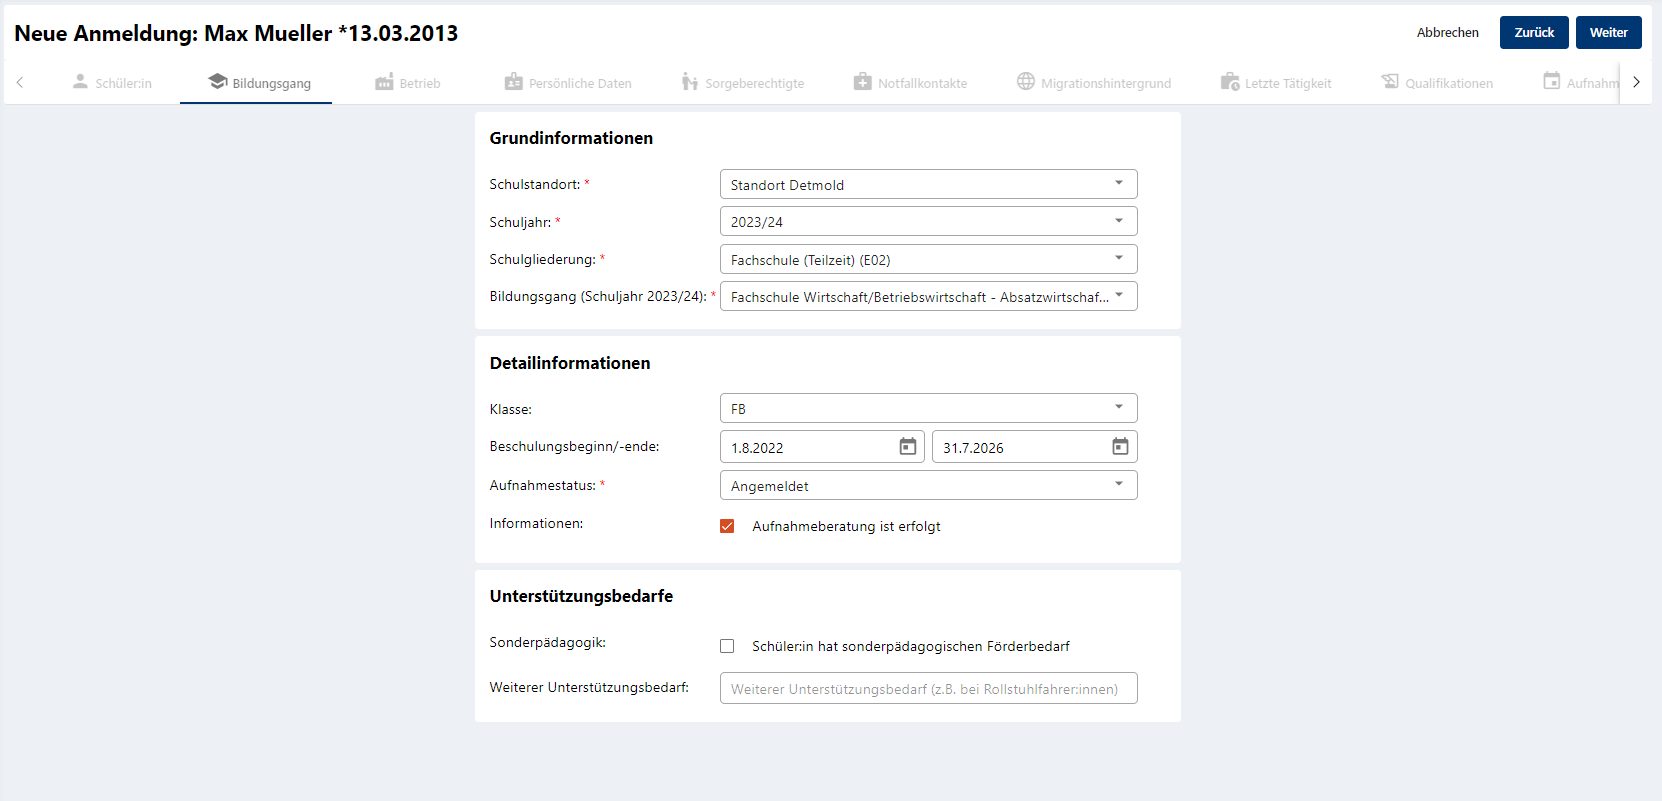
\includegraphics{bildungsgang}
    %\end{adjustbox}
%\end{figure}

Um den Realitätsbezug zu gewährleisten, unterschieden sich die Datensätze je nach Schule, insbesondere in Bezug auf das Geburtsjahr, das an die jeweilige Schulstufe angepasst wurde. So wurde für Bewerbungen an der Primarstufe das Geburtsdatum so gewählt, dass das Schulkind zum Zeitpunkt des ersten Schultages 6 Jahre alt wäre. Im Falle einer Bewerbung für die Sekundarstufe 1 war das Schulkind 10 Jahre und für die Sekundarstufe 2 entsprechend 16 Jahre alt.
Hierzu wurden so genannte Anmeldeformulare der jeweiligen Schule verwendet, die mit Ausnahme des Geburtsdatums und des zu besuchenden Bildungsgangs mit identischen Inhalten ausgefüllt wurden (s. Abbildung \ref{fig:konstellationenv3}).

Zu beachten ist, dass alle Datensätze fiktiv waren, um etwaige Probleme hinsichtlich der Vertraulichkeit zu vermeiden. Dies wurde den Teilnehmern vor Beginn der Aufgaben explizit mitgeteilt.

\subsection{Bereitstellung des Fragebogens}

Im Vorfeld der Untersuchung wurde der Fragebogen den Studienteilnehmern nicht vorab zur Verfügung gestellt. In den initialen Telefongesprächen wurde jedem Teilnehmer ausdrücklich mitgeteilt, dass keine spezielle Vorbereitung für die Teilnahme an der Studie erforderlich sei. Die Software und der Zweck der Studie wurde jedem Teilnehmer in diesem Zuge ebenfalls kurz dargelegt.

Darüber hinaus wurden in diesen Gesprächen die Software \textit{Schüler Online} und der Zweck der Studie den Teilnehmern ausführlich erläutert. Dies gewährleistete, dass jeder Teilnehmer über den Kontext und die Ziele der Studie informiert war und eine Vorstellung von dem hatte, was von ihm oder ihr erwartet wurde.

\subsection{Rollenverteilung während der Studie}

Während der Durchführung der Studie gab es zwei Hauptrollen innerhalb des Forschungsteams: den Interviewer und den Schreiber. Der Interviewer, der die Software mehrere Jahre mitentwickelt hat, war mit den funktionalen Aspekten des Systems gut vertraut, hatte jedoch keine umfangreichen praktischen Erfahrungen hinsichtlich Interviewtechniken. Diese Rolle wurde durch eine Person besetzt, deren Aufgabe es war, die Teilnehmer durch die Aufgaben zu leiten und die Diskussion während des Interviews zu lenken.

Die Rolle des Schreibers wurde durch zwei Personen wahrgenommen, die sich abwechselten. Schreiber A nahm an den Interviews 1 und 4 teil, während Schreiber B an den Interviews 2, 3 und 5 präsent war. Beide Schreiber hatten grundlegende Kenntnisse der Software, die sie während des ersten Jahres ihrer Beteiligung an der Entwicklung der Software erworben hatten.

Die Hauptaufgabe der Schreiber war es, während der Interviews Notizen zu machen und die Reaktionen der Teilnehmer sowie relevante Beobachtungen zu dokumentieren. 

\subsection{Durchführung der Studie}

Die Implementierung der Studie wurde vor Ort in den Schulen durchgeführt. Der Interviewer und der Schreiber trafen sich persönlich mit den Teilnehmern. Beide stellten sich kurz vor und erläuterten den Zweck der zu untersuchenden Software.

Für die Interviews suchten sie sich innerhalb des Raums einen Ort aus, von dem aus sie sowohl den Monitor als auch den Probanden gut beobachten konnten. Während des Interviews stellte der Interviewer sowohl die Fragen aus dem Fragebogen als auch zusätzliche klärende Fragen. Der Notierer hingegen konzentrierte sich hauptsächlich darauf, die Antworten und Beobachtungen zu dokumentieren.

Die Beobachtung der Aufgabenbearbeitung und des Verhaltens der Teilnehmer war sowohl dem Interviewer als auch dem Notierer zugeordnet. Um ein realistisches Szenario zu gewährleisten, wurden keine fachlichen Rückfragen der Studienteilnehmer beantwortet - sie mussten sich, ähnlich wie in einer realen Arbeitsumgebung, auf die Dokumentation und ihre eigenen Ressourcen verlassen.

Den Teilnehmern wurde versichert, dass das Ziel der Studie war, die Software und nicht den Anwender zu testen. Das Interview und die Beobachtung fanden gleichzeitig statt und dauerten zwischen einer und drei Stunden.

Die Teilnehmer agierten entsprechend des \textit{Meister-Schüler-Modells} in der Rolle des Meisters, von denen der Schüler (Interviewer) lernen kann.\cite{Seibert-Giller,jacobsen} Sie wurden dementsprechend nicht in ihren Ansichten korrigiert.

Um in dieser Ausarbeitung die Antworten und Beobachtungen zuordenbar zu machen, sind die Resultate der Sekretärinnen des Gymnasiums (1), der Realschule (2), der Förderschule (3), der Grundschule (4) und des Berufskollegs (5) konsequent und analog zu ihrer Indexziffer den Anhängen \ref{section-InterviewGymnasium} - \ref{section-InterviewBerufskolleg} zugeordnet.

In der ersten Durchführung mit dem Gymnasium (1) gab es die Besonderheit, dass  in Anlehnung an die Empfehlung des Leitfaden Usability ein erfahrener Requirements Engineer (der Product Owner der Software) mittels Anruf zugeschaltet wurde, der \glqq in Form einer Supervision die Gesprächssituation beobachtet, bewertet und anschließend mit dem Beobachteten [besprochen hat]\grqq{}\cite{dakks}.

In drei Fällen (Gymnasium (1), Realschule (2) und zeitweise bei der Förderschule(3)) waren bei der Durchführung der Interviews zwei Mitarbeiter vonseiten der Studienteilnehmer anwesend. Es wurde die Entscheidung getroffen, das Interview nur mit dem vorab rekrutierten Teilnehmer durchzuführen. Kommentare und Diskussionen zwischen den Mitarbeitern waren jedoch zulässig, um ein realistischeres Szenario zu belassen. Die gesammelten Daten wurden ausschließlich aus den Ansichten, Antworten und Beobachtungen des Interviewpartners erfasst, nicht von dem weiteren Mitarbeiter. Die Interviews wurden direkt in Microsoft Word dokumentiert. Es wurden keine Audio- oder Filmaufnahmen erstellt.

\subsection{Nachbereitung und Auswertung der Studie}

Unmittelbar nach Abschluss der Interviews wurde eine erste Nachbearbeitung der gesammelten Daten durchgeführt. Hierbei wurden unklare oder zu kurz formulierte Notizen präzisiert und ausführlicher beschrieben. Es ist wichtig zu betonen, dass diese Nachbearbeitung nur für Einträge vorgenommen wurde, bei denen eine eindeutige Interpretation möglich war. Bei Notizen, bei denen das Potenzial für Fehlinterpretationen bestand oder die im Nachhinein unklar blieben, wurden keine Änderungen vorgenommen. Sie wurden in ihrer ursprünglichen Form beibehalten, um die Möglichkeit von Missverständnissen zu minimieren.

Für die Auswertung der gesammelten Daten wurden keine speziellen Analysetools oder ähnliche Instrumente verwendet. Die Auswertung erfolgte lediglich bei den Notizen, die unmissverständlich waren und bei denen man keine Fehlinterpretationen beim Ausformulieren machen konnte. Bei Punkten, die potenziell fehlinterpretiert werden konnten oder im Nachhinein unklar waren, wurden keine Ausformulierungen durchgeführt, sondern die Notiz so belassen wie sie mitgeschrieben wurde. Verständnis der Benutzererfahrungen und -bedürfnisse zu gewinnen.

%todo: Die Ergebnisse der unterschiedlichen Schulen wurden jedoch händisch miteinander auf Gemeinsamkeiten und Kontroversen verglichen. 


\subsection{Materialien und Ressourcen}

Für die Durchführung der Studie war vonseiten der Teilnehmer lediglich ein Computer mit Internetzugang erforderlich, um den Zugriff auf die Anwendung zu ermöglichen. Darüber hinaus war kein zusätzliches Material notwendig.
Vonseiten der Moderation wurden ein Laptop für Notizen und der ausgearbeitete Fragebogen sowie die Anmeldeformulare verwendet

%  Ethik: Welche ethischen Gesichtspunkte wurden bei der Durchführung des Interviews berücksichtigt, z.B. in Bezug auf Datenschutz oder Anonymität?
 
 
% In diesem Kapitel solltest du die Methoden und Techniken, die du zur Durchführung deiner Projektarbeit verwendest, beschreiben und begründen. Hier sollten auch die Einzelheiten zur Durchführung des leitfadengestützten Interviews enthalten sein.
% Für das leitfadengestützte Experteninterview solltest du in der Methodik deiner Projektarbeit den Ablauf und die Durchführung des Interviews beschreiben. Hierbei sollst du beispielsweise folgende Punkte erwähnen:
% Teilnehmer: Wer wurde für das Interview ausgewählt und warum? Wie viele Experten wurden befragt? 

% material
% Wie haben wir den Fragebogen erstellt? 
% Schulleiter zeigt nochmal weitere Aspekte auf
% Offene Fragen gemacht => Warum offene Fragen
% induktives vorgehen
% ich habe jedes Sekretärin vorher telefonisch gesprochen

% Fragebogen ist delegiert ans Team und ein Zwischenergebnis. Ist ein Ergebnis eines Expertenteams für dieses Programm
% Experten sind Material


% ggf. der fixierte Nutzungskontex 
\pagebreak
\section{Ergebnisse}

\textbf{In welchem Umfang besitzen Sie Vorerfahrungen mit Schüler Online 1.0?}\\
Im Hinblick auf die ersten Vorerfahrungen mit der Anwendung Schüler Online 1.0 offenbarten sich signifikante Unterschiede zwischen den befragten Sekretärinnen unterschiedlicher Schultypen.

Die Sekretärin des Gymnasiums (1) konnte aufgrund regelmäßiger Datenpflegeaktivitäten, die halbjährlich im Zuge von Schulwechseln zu den örtlichen Berufskollegs stattfanden, bereits praktische Erfahrung mit der Anwendung vorweisen. Zusätzlich berichtete sie von indirekten Erfahrungen, die sie durch einen kollegialen Austausch erwarb, in dessen Rahmen ein Kollege ein Praktikum in einem Berufskolleg absolviert hatte.

Im Gegensatz dazu gaben die Sekretärinnen der Realschule (2), der Förderschule (3) und der Grundschule (4) an, keinerlei Vorerfahrungen mit Schüler Online 1.0 zu haben.


\textbf{In welchem Umfang besitzen Sie Vorerfahrungen mit der neuen Software?}\\
Bezüglich der Vorerfahrungen mit der neuen Software berichteten die Sekretärinnen unterschiedlich. Die Sekretärin des Gymnasiums (1), der Realschule (2), der Grundschule (4) sowie die des Berufskollegs (5) gaben an, keinerlei vorherige Erfahrung mit dem System zu haben.

Anders äußerte sich die Sekretärin der Förderschule (3). Sie hatte bereits einen ersten Blick auf das System geworfen, die Elternseite eingeschlossen. Sie gab an, dass sie sich bereits auf der Seite angemeldet und eingeloggt hatte. Sie wünschte sich eine Exportfunktion zu Excel und \textit{SchILD} und wies darauf hin, dass sie eine explorative Herangehensweise an neue Software bevorzugt(\glqq Ich probier mal lieber, als mir was anzuhören\grqq{}). Darüber hinaus merkte sie an, dass sie die Daten für die Aufgaben zwei und drei bereits vorfand(\glqq Die (Datensätze unter Anmeldungen) sind einfach so reingekommen\grqq{}).

\textbf{Welche Probleme können bei herkömmlichen, nicht-digitalen Bewerbungen von Schülern auftreten?}\\
Hinsichtlich der Dateneingabe durch Eltern und Schüler lieferten die Sekretärinnen verschiedener Schultypen diverse Beobachtungen und Erfahrungen.

Die Sekretärin des Gymnasiums (1) stellte fest, dass sich Eltern beim Einschulungsjahr der Kinder oft verrechnen und dass Schüler gelegentlich versehentlich falsche Daten eingeben, ohne dabei jedoch böswillige Absichten zu haben.

Demgegenüber äußerte die Sekretärin der Realschule (2) Bedenken hinsichtlich verschiedener Problembereiche: Falsch ausgefüllte oder fehlende Angaben, Unleserlichkeit sowie inkorrekte Daten wurden als häufige Fehlerquellen identifiziert. Darüber hinaus wies sie darauf hin, dass bestimmte Fachbegriffe wie \glqq Konfession\grqq{} oder \glqq Schulformempfehlung\grqq{} für Schüler möglicherweise nicht verständlich seien. Sie stellte fest, dass einige Schüler absichtlich falsche Angaben machen würden und verwies auf die Komplexität der Themen Sorgeberechtigung und Datenschutz. Dies steht im Gegensatz zur Aussage der Gymnasiums-Sekretärin, die lediglich versehentliche Fehler thematisiert hatte.

Die Sekretärin der Förderschule (3) unterstrich die Problematik der Lesbarkeit, insbesondere bei handschriftlich notierten E-Mail-Adressen.

Die Sekretärinnen der Grundschule (4) und des Berufskollegs (5) gaben an, dass unvollständige Einträge, unleserliche Handschrift und fehlende Unterschriften ebenfalls zu den häufigsten Schwierigkeiten bei der Dateneingabe zählten.

\footnote{Negativbescheinigungen sind Bescheinigungen über das alleinge Sorgerecht}


\textbf{Wer nutzt das System hauptsächlich an Ihrer Schule?}\\
Die Sekretariate aller fünf Schulen (1, 2, 3, 4, 5) nutzten das System. Darüber hinaus verwendete bei den Sekretärinnen der Förderschule (3) und des Berufskollegs (5) auch die Verwaltung die Software. Zusätzlich zu Sekretariat und Verwaltung wurden bei der Sekretärin des Berufskollegs (5) die Lehrer einbezogen, die über Aufnahmeentscheidungen bestimmten. Die Sekretärin der Förderschule (3) fügte hinzu, dass ihre Schule über mehrere Standorte verfüge.

% todo: \textbf{Welche (Teil-)Faktoren bestimmen das Abschließen einer Bewerbung, sodass sie diese nicht mehr bearbeiten müssen?}\\

\textbf{Beschreiben Sie die Ausgangssituation die vorliegt, bevor Sie die Aufgabe \glqq Bewerbung eines Schülers\grqq{} durchführen.}\\
Die Sekretärin des Gymnasiums (1) erklärte, dass ein Anmeldeformular vorliegen müsse. Alle Datenfelder auf dem Papierformular sollten ausgefüllt sein und wichtige Unterlagen eingereicht werden. Bei Unleserlichkeit würde telefonisch nachgefragt werden.

Die Sekretärin der Realschule (2)  \textit{SchILD} erte, dass die Entscheidung über die Aufnahme eines Kindes auf der Schulempfehlung und vorausgehenden Gesprächen mit der Schulleitung basiere. Im Falle von Sprachbarrieren der Eltern würde das Formular gemeinsam ausgefüllt. Mehrfachanmeldungen sollten vermieden werden und würden in der Regel bei Kennenlernterminen auffallen. Sie erklärte, dass die Schulen der Region eine spezielle Methode anwendeten, um dies sicherzustellen (mittels farbiger Formulare).

Die Sekretärin der Förderschule (3) gab an, dass im Vorfeld mit den Eltern telefoniert würde. Das Kind müsse im Schuleinzugsgebiet leben. Eine Information über die Diagnose Autismus könnte oft schon als Entscheidungsgrundlage für die Eignung des Kindes dienen, allerdings könnten in einigen Fällen auch Gutachten erforderlich sein.

Die Sekretärin der Grundschule (4) berichtete, dass die Eltern ein mehrseitiges Anmeldeformular ausfüllen würden, welches sie dann digitalisiere. Gelegentlich würden die Formulare auch per E-Mail eingereicht.

Die Sekretärin des Berufskollegs (5) beschrieb den Prozess als umfangreich, beginnend mit der Bewerbung des Schülers bis hin zu abrufbaren Daten im Schulverwaltungsprogramm.

\textbf{(DAkkS) Welche fachlichen und technischen Qualifikationen sind zur Bewältigung der Aufgabe erforderlich (Aufgabenbewältigung / Softwarenutzung)? Welche Vorkenntnisse fehlen ggf.?}\\
Die Sekretärin des Gymnasiums (1) äußerte, dass zur Bewältigung der Aufgabe keine besonderen fachlichen oder technischen Kenntnisse erforderlich seien. Grundlegende Lesekompetenz sei ausreichend, spezifisches Wissen über das Schulsystem hingegen nicht notwendig.

Ähnlich äußerte sich die Sekretärin der Realschule (2). Sie betonte, dass nicht einmal Internet-Affinität Voraussetzung sei, allerdings sollte man die Bereitschaft mitbringen, sich mit der Software auseinanderzusetzen und sie ausprobieren zu wollen.

Die Sekretärin der Förderschule (3) nannte technische Grundvoraussetzungen wie einen Computer und Internetzugang. Ihrer Ansicht nach könnten die Sekretärinnen mit der Software umgehen, sobald sie einmal damit gearbeitet haben. Auch sie betonte, dass Kenntnisse des Schulgesetzes nicht zwingend notwendig seien, jedoch sei ein Bewusstsein für Datenschutzfragen wichtig.

Die Sekretärin der Grundschule (4) sprach die Vorteile von Kenntnissen im Umgang mit MS Office und grundlegendem Wissen im Schulgesetz an, obgleich diese nicht zwingend notwendig seien. Sie unterstrich ebenfalls die Bedeutung von Sensibilität in Bezug auf den Datenschutz.

Die Sekretärin des Berufskollegs (5) betonte, dass möglicherweise Schulungen zur Vertiefung des fachlichen Wissens, insbesondere für die Schulverwaltung, fehlen könnten. Sie stellte auch heraus, dass ein Verständnis für die spezifischen Bildungsangebote der eigenen Schule wichtig sei.


\subsection{Zu Beginn der Durchführung}
Zu Beginn der Durchführung der Aufgaben mit der neuen Software zeigten sich bei mehreren Sekretärinnen Schwierigkeiten in der Navigation. Die Sekretärin des Gymnasiums (1) navigierte beispielsweise auf eine leere Seite und konnte den Sinn und Zweck der Menüpunkte \glqq Schüler:innen\grqq{} und \glqq Anmeldungen\grqq{} nicht korrekt differenzieren. Obwohl ihre Aufgabe darin bestand, eine Anmeldung zu erfassen, konnte sie aufgrund der bereitgestellten Informationen nicht richtig navigieren.

Sowohl die Sekretärin des Gymnasiums (1) als auch die der Förderschule (3) mussten dahingehend instruiert werden, wie sie die Aufgabe beginnen können. Beide waren anfangs dabei, einen inkorrekten Prozess zu starten.

Die Sekretärin des Berufskollegs (5) navigierte durch mehrere Menüpunkte, konnte jedoch letztendlich auf die korrekte Seite gelangen. 

\textbf{(DAkkS) Welche Arbeitsschritte sind durchzuführen?}\\
Die Sekretärin des Gymnasiums (1) beschrieb den Prozess in drei Schritten: Zuerst müsse der Schüler im System gesucht werden, dann würden die Daten des Schülers erfasst. Anschließend müsse dem Schüler eine Information übermittelt werden.

Die Sekretärin der Realschule (2) betonte die Bedeutung der persönlichen Anwesenheit des Schülers an der Schule.

Für die Sekretärin der Förderschule (3) umfasste der Prozess mehrere Schritte: Erst müsse geklärt werden, ob ein Rundgang durchgeführt wurde. Danach würden die Daten aufgenommen und das Gutachten für die Akten angefordert. Ein kurzes Kennenlernen und die Entscheidung, in welche Klasse das Kind käme, gehörten ebenso zu den Arbeitsschritten.

Die Sekretärin der Grundschule (4) erläuterte, dass die Eltern zunächst ins Sekretariat kämen, wo ein Gespräch stattfände. Anschließend würden die Daten erfasst und Unterlagen eingereicht. Letztendlich würde eine Schülerakte angelegt.

Die Sekretärin des Berufskollegs (5) führte aus, dass die Daten zuerst in Papierform erfasst und dann ins System eingetragen würden.


\textbf{(DAkkS) Welche Hilfsmittel sind erforderlich (für die Aufgabenbewältigung / zur Softwarenutzung)? Welche davon fehlen ggf., welche sind zusätzlich gewünscht?}\\
Für die Sekretärin des Gymnasiums (1) sind Kopier- und Einfügefunktionalitäten wichtig, um Daten aus anderen Programmen wie E-Mail oder PDF-Reader übertragen zu können.

Die Sekretärin der Förderschule (3) nutzt Google Maps zur Adressrecherche als unterstützendes Hilfsmittel.

Die Sekretärin des Berufskollegs (5) spricht den Bedarf an Laptops und einer Kurzanleitung für den Einstieg in die Softwarenutzung an.

Es wurden keine fehlenden Hilfsmittel oder zusätzlich gewünschte Tools spezifisch angegeben.

\textbf{(DAkkS) Welche Ergebnisse / Teilergebnisse entstehen und wie werden diese ggf. verwertet / weitergeführt?}\\
Die Sekretärin der Grundschule (4) erklärt, dass am Ende des Prozesses der Schüler angemeldet ist. Die in der Anwendung erfassten Daten können bei Bedarf für weitere schulische Prozesse herangezogen werden.

Die Sekretärin des Berufskollegs (5) stellt heraus, dass nach Abschluss des Prozesses alle notwendigen Daten für die Bewerbung des Schülers erfasst sein sollten. Sie betont insbesondere die Wichtigkeit der Erfassung der vorherigen Schule, da es sehr aufwändig wäre, diese Information nachträglich herauszufinden. Die erfassten Daten bilden somit eine wesentliche Grundlage für die weitere schulische Laufbahn und Verwaltungsprozesse des Schülers.

\textbf{(DAkkS) Welche wichtigen Sonderfälle müssen berücksichtigt werden? (bzw. fallen dem Benutzer spontan ein; z. B. zur Arbeitsteilung / Zusammenarbeit)}\\
Die Sekretärin des Gymnasiums (1) weist darauf hin, dass Wechsel innerhalb des Schuljahres und das Wiederholen von Stufen berücksichtigt werden müssen. Bei Flüchtlingskindern sind möglicherweise nicht alle erforderlichen Daten vorhanden. Sie stellt besondere Situationen heraus, wie langfristige Beurlaubungen oder Fälle, in denen unklar ist, in welche Klasse ein Kind gehen soll. Ein Beispiel wäre ein Kind, das eine Therapie macht und nicht am regulären Schulbetrieb teilnimmt, aber dennoch wegen der Schulpflicht an der Schule angemeldet werden muss. Solche Kinder werden oft in der Klinik unterrichtet.

Die Sekretärin der Realschule (2) weist darauf hin, dass Unterricht in der Herkunftssprache im Voraus beim Schulamt angemeldet werden muss. Hierfür gibt es jährlich ein neues Formular, das unterschrieben werden muss.

Die Sekretärin der Förderschule (3) erklärt, dass in Förderschulen keine spezifischen Schulstufen existieren, was bei der Anmeldung berücksichtigt werden muss.

Die Sekretärin der Grundschule (4) betont, dass besondere Fälle wie unterschiedliche Staatsangehörigkeiten und bestimmte Sorgerechtssituationen die Anmeldung komplizieren können.

Die Sekretärin des Berufskollegs (5) identifiziert Schüler mit Förderbedarf als Sonderfälle. Sie merkt auch an, dass manche Schüler in ihrem Alter unsicher sind, ob sie sich als männlich oder weiblich identifizieren. Des Weiteren stellt sie fest, dass bei minderjährigen Schülern eine Unterschrift der Eltern erforderlich ist. Ein weiterer Sonderfall sind Schüler, die sich zu spät bewerben und möglicherweise nicht die notwendigen Voraussetzungen für bestimmte Bildungsgänge erfüllen. Sie stellt fest, dass wenige Schüler genau wissen, was sie lernen wollen oder welchen Bildungsgang sie besuchen möchten.


\subsection{Während der Durchführung}
%todo überleitungstext \textbf{Für jeden Tab / Seite: Welche Seiteninhalte sind unverständlich?}\\

\textbf{\glqq Schüler\grqq{}-Tab}\\
Alle Studienteilnehmer hatten Schwierigkeiten zu verstehen, wofür das Feld \glqq ID-Schlüssel\grqq{} gedacht ist.

Die Sekretärin des Gymnasiums (1) konnte den Zweck der Schülersuche-Funktion nicht nachvollziehen.


\textbf{Anmerkungen zum Tab \glqq Bildungsgang\grqq{}}\\
Für die Sekretärin des Gymnasiums (1) war das Dropdown-Feld \glqq Klasse\grqq{} unklar, da keine Daten vorhanden waren und noch nicht feststand, welche Klassen es geben würde. Sie wählte den Status \glqq Warteliste\grqq{}, um die Bewerbung als \glqq in Bearbeitung\grqq{} zu markieren und konnte nicht nachvollziehen, warum in der Anwendung vermerkt werden soll, dass eine Aufnahmeberatung stattgefunden hat.

Die Sekretärin der Realschule (2) hätte den Begriff \glqq Neuaufnahme\grqq{} in der Auswahl für den Aufnahmestatus erwartet, da diese Terminologie auch bei \glqq  \textit{SchILD} \grqq{} verwendet wird. Sie merkte an, dass die Telefonnummervorwahl nicht zum Ort passte und dass sie in der Realität noch einmal bei der anderen Telefonnummer nachfragen würde. Sie hatte auch Schwierigkeiten, das Beschulungsbeginndatum korrekt einzugeben.

Die Sekretärin der Förderschule (3) hielt die Sortierung der Schuljahre für nicht sinnvoll und stellte fest, dass man mitunter keine medizinischen Informationen erfassen darf.

Die Sekretärin der Grundschule (4) war verwirrt durch die Meldung, dass ein Antrag auf vorzeitige Einschulung stattfindet und fand die Bildungsgangbezeichnungen verwirrend.

Die Sekretärin der Berufsschule (5) hatte Diskussionen mit einer Kollegin, wie das Feld \glqq Schuljahr\grqq{} zu interpretieren ist. Sie hatte eine andere Meinung als die Kollegin, dass es sich dabei um das aktuelle Schuljahr handelt und nicht um das Schuljahr, das der Schüler zuvor besucht hat. Der Anmeldestatus war für sie nicht klar interpretierbar.

\textbf{Anmerkungen zum Tab \glqq Persönliche Daten\grqq{}}\\
Die Sekretärin des Gymnasiums (1) trug die Hausnummer zunächst intuitiv zusammen mit der Straße ins Feld \glqq Straße\grqq{} ein, anstatt ins Feld \glqq Hausnummer\grqq{}. Sie gab auch die E-Mail-Adresse des Sorgeberechtigten in das E-Mail-Feld des Schülers ein. Sie merkte an, dass sie es bevorzugen würde, wenn der Tab \glqq Persönliche Daten\grqq{} vor dem Tab \glqq Bildungsgang\grqq{} kommen würde, so wie es bei \glqq  \textit{SchILD} \grqq{} der Fall ist. Sie schlug auch vor, dass der Eintrag für \glqq Staat\grqq{} standardmäßig mit \glqq Deutschland\grqq{} vorbelegt sein sollte. Sie wünschte sich außerdem einen Hinweis, dass bei Sek1-Schülern grundsätzlich die Telefonnummer der Sorgeberechtigten und bei Sek2-Schülern die des Schülers erwartet wird.

Die Sekretärin der Realschule (2) fand die Erfassung von Ortsteilen interessant.

Die Sekretärin der Förderschule (3) überprüft unbekannte Straßen mithilfe von Google Maps auf ihre Existenz. Sie schlug vor, dass es sinnvoll wäre, wenn Eltern angeben könnten, zu welchen Zeiten sie telefonisch erreichbar sind. Sie fände es auch gut, wenn mehrere Telefonnummern für Notfälle erfasst werden könnten.

Die Sekretärin der Berufsschule (5) wünschte sich eine Anzeige, die darauf hinweist, ob der Schüler volljährig ist. Sie hatte Schwierigkeiten mit der Suche nach der Postleitzahl-Ort-Kombination.

\textbf{Anmerkungen zum Tab \glqq Sorgeberechtigte\grqq{}}\\
Die Sekretärin des Gymnasiums (1) hielt es für wichtig, einen Nachweis dafür zu haben, ob eine Person das alleinige Sorgerecht hat oder ob beide Unterschriften vorhanden sind, um zu verhindern, dass sich eine Person über die andere hinwegsetzt. Sie hätte erwartet, dass es eine Funktion zur Datenübernahme der Adressdaten aus den persönlichen Daten des Schülers gibt. Sie war auch unsicher über den Zweck des Postfachs. Sie war verärgert, als der Sorgerechtsprozess durch einen versehentlichen Klick neben das Popup abgebrochen wurde, und forderte, dass es nicht möglich sein sollte, Daten zu verlieren, sei es durch danebenklicken oder Ausloggen.

Die Sekretärin der Realschule (2) trug die Hausnummer auch intuitiv zusammen mit der Straße in das Feld \glqq Straße\grqq{} ein.

Alle Sekretärinnen außer 5 (also 1, 2, 3 und 4) versuchten, die Straße in das Feld \glqq Adressart\grqq{} einzugeben. Die Sekretärin der Förderschule (3) erklärte auf Nachfrage, dass sie intuitiv die folgende Eingabereihenfolge erwartet hätte: Staat => Postleitzahl/Ort => Straße.

Der \glqq Erstellen\grqq{}-Button wurde unterschiedlich interpretiert. Die Sekretärin der Förderschule (3) interpretierte ihn im Sinne von \glqq Speichern\grqq{}, während die Sekretärin der Hauptschule (4) annahm, dass damit ein weiterer Sorgeberechtigter angelegt werden kann, was sie auf das Plus-Symbol zurückführte.

Die Sekretärin der Berufsschule (5) empfand das Erfassungsformular für die Sorgeberechtigten im Vergleich zu den anderen Formularen als unattraktiv und unübersichtlich.

\textbf{Anmerkungen zum Tab \glqq Notfallkontakte\grqq{}}\\
Die Sekretärin der Realschule (2) schlug vor, dass es hilfreich wäre, die Art der Telefonnummer (im Sinne von dienstlich, privat, mobil) für die Notfallkontakte hinterlegen zu können und mehrere Telefonnummern einer Person zuzuordnen. Sie konnte zeitweise nicht erkennen, wie sie den Datensatz speichern kann, da das Autocomplete-Dropdown-Feld den Speichern-Button versteckte. Sie nahm dieses Feld nicht als ein Feld wahr, das man benutzerdefiniert ausfüllen kann, sondern als ein Feld, in dem man zwingend einen der vorgeschlagenen Werte auswählen muss.

Die Sekretärin der Förderschule (3) versuchte, mehrere Nummern in ein Feld einzugeben, was ihr nicht gelang. Wie 2 schlug sie vor, dass es möglich sein sollte, Erreichbarkeitszeiträume einzutragen. Sie wies auch darauf hin, dass es wichtig sei, die Rolle des Notfallkontakts zu erfassen, um im Notfall beurteilen zu können, ob sensible Informationen weitergegeben werden dürfen. Eine Rangfolge der Notfallkontakte hielt sie nicht für sinnvoll. Sie hätte erwartet, die Notfallkontakte früher im Prozess zu sehen.

Die Sekretärin der Hauptschule (4) empfand die Eingabe der Notfallkontakte als unpraktisch, da sie die gleichen Daten wie bei den Sorgeberechtigten eingeben musste. In \textit{SchILD} werden diese Daten automatisch übernommen.

\textbf{Anmerkungen zum Tab \glqq Migrationshintergrund\grqq{}}\\
Die Sekretärin des Gymnasiums (1) äußerte Zufriedenheit mit dem Abschnitt zum Migrationshintergrund und betonte, dass alle wichtigen Informationen vorhanden seien. Sie war jedoch der Meinung, dass das Eingabefeld angezeigt werden sollte, selbst wenn die Option \glqq Migrationshintergrund liegt nicht vor\grqq{} ausgewählt ist.

Die Sekretärin der Gesamtschule (5) stellte die Definition von \glqq Migrationshintergrund\grqq{} in Frage. Sie war sich unsicher und spekulierte darüber, ab wann ein Migrationshintergrund angenommen wird.

\textbf{Anmerkungen zum Tab \glqq Letzte Tätigkeit\grqq{}}\\
Die Sekretärin des Gymnasiums (1) kritisierte die Reihenfolge der Bereiche und schlug vor, dass die \glqq Letzte Tätigkeit\grqq{} innerhalb des Abschnitts \glqq Schüler-Daten\grqq{} erfasst werden sollte, da es sich hierbei um ergänzende Informationen zur Person handelt. Sie hatte Schwierigkeiten mit der Suche nach der letzten Schule, da die Suche eine Checkbox überdeckte und die Sortierung der Ergebnisse ihrer Meinung nach die lokale Umgebung bevorzugen sollte.

Die Sekretärin der Gemeinschaftsschule (3) hielt den Tab \glqq Letzte Tätigkeit\grqq{} für überflüssig, da ein Kind, das sich für die Grundschule anmeldet, noch keinen Schulabschluss haben kann. Sie war verwirrt und konnte nicht unterscheiden, ob die letzte Tätigkeit des Schülers oder des Sorgeberechtigten erfragt wird. Die angestrebte Schulstufe wurde von ihr als letzte Schulstufe interpretiert.

Die Sekretärin der Gesamtschule (5) hatte Schwierigkeiten, eine einmal ausgewählte Grundschulempfehlung wieder zu entfernen. Sie wies darauf hin, dass das Feld \glqq Angestrebte Schulstufe\grqq{} und der Tab \glqq Letzte Tätigkeit\grqq{} einander zu widersprechen scheinen.

\textbf{Anmerkungen zum Tab \glqq Qualifikationen\grqq{}}\\
Die Sekretärin der Gesamtschule (5) stellte fest, dass in der Liste der Qualifikationen einige Schulabschlüsse, wie beispielsweise der Hauptschulabschluss, fehlten. Sie äußerte Kritik und regte eine Überarbeitung der Auswahlmöglichkeiten an.

\textbf{Anmerkungen zum Tab \glqq Termine\grqq{}}\\
Sekretärin 5 konnte den Zweck der Seite \glqq Termine\grqq{} nicht erkennen. Sie gab an, dass sie ohnehin keine Zeit hätte, 500 Personen zu Terminen einzuladen. Sie merkte jedoch an, dass einige Bildungsgangleitungen vorab Gespräche mit den Schülern führen möchten.

\textbf{Anmerkungen zum Tab \glqq Bemerkungen\grqq{}}\\
Sekretärin 2 äußerte Unsicherheit darüber, wer Zugriff auf die internen Notizen hat. Sie definierte das Feld \glqq Interne Notiz\grqq{} und \glqq Bemerkung für Schüler*in\grqq{} als \glqq Anmerkung ist unsere Meinung, Bemerkungen sind Fakten\grqq{}. Sekretärin 4 war sich ebenfalls unsicher, welche Informationen dem Schüler zugänglich sind. Im Gegensatz zu 2 interpretierte 4, dass die \glqq Interne Notiz\grqq{} nur für die Schule sichtbar ist und das \glqq Bemerkung\grqq{}-Feld auch vom Kind gesehen werden kann, fühlte sich aber durch den Infotext oben im Formular verwirrt.

Sekretärin 3 machte darauf aufmerksam, dass sensible Informationen, wie zum Beispiel Behinderungen, möglicherweise nicht erfasst werden dürfen. Sie betonte die Notwendigkeit einer Benutzerführung, die das Bewusstsein für gesetzliche Anforderungen stärkt.

Sekretärin 5 war überrascht, dass dieser Tab erschien, da sie zuvor nicht bemerkt hatte, wie weit sie im Prozess fortgeschritten war. Sie stellte fest, dass dieser Tab zuvor aufgrund des Overflow-Verhaltens des Browsers verdeckt war.

Sekretärin 1 gab an, dass sie den Tab \glqq Anmerkungen\grqq{} an einer früheren Stelle im Prozess erwartet hätte.

\textbf{Anmerkungen zum Tab \glqq Zusammenfassung\grqq{}}\\
Sekretärin 1 erlebte eine unklare Fehlermeldung beim Klick auf \glqq Speichern\grqq{}. Sie wünscht sich klarere Anweisungen zur Fehlerbehebung und einen direkten Fokus auf das fehlerhafte Feld.
Sekretärin 2 stellte eine Verzögerung beim Laden der Inhalte fest. Sie befürchtet, dass die per E-Mail gesendete Bestätigungsmeldung mit der Formulierung \glqq Angemeldet\grqq{} falsche Erwartungen bei den Schülern wecken könnte. Sie war sich auch unsicher, ob das Schuljahr korrekt erfasst wurde und merkte an, dass noch eine Unterschrift von den Eltern für die Anmeldung erforderlich ist.
Sekretärin 3 interpretierte die Meldung auf der Zusammenfassungsseite als \glqq Die Mutter wurde kontaktiert\grqq{}.
Sekretärin 4 nahm an, dass die Anmeldung des Kindes als \glqq vorzeitige Einschulung\grqq{} gekennzeichnet wurde, was sie als Fehler ansah. Sie war sich auch unsicher, ob sie nun eine \glqq Anmeldung\grqq{} oder nur eine \glqq Bewerbung\grqq{} eingereicht hat. Sie bemerkte, dass Informationen zu wichtigen Themen wie dem Nachweis des Masernschutzes oder der Betreuung für beispielsweise die offene Ganztagsschule fehlten.
Sekretärin 5 kritisierte den Informationsgehalt der Seite. Ihrer Meinung nach sind zu viele Informationen im Panel \glqq Bildungsgang\grqq{} enthalten, insbesondere das Kürzel des Bildungsgangs, das für sie schwer zu verstehen war.



Nach der Durchführung:

\textbf{Konnten Sie die Aufgabe aus Ihrer Sicht erfolgreich und vollständig abschließen? Falls nein - was hat Sie daran gehindert?}\\

\textbf{Wie effektiv unterstützt die Webanwendung Sie bei der Aufgabe?  Gab es positive oder negative Erfahrungen?}\\

\textbf{Haben Sie sämtliche Inhalte der Aufgabe verstanden? Gab es Stellen, an denen Sie sich mehr Unterstützung gewünscht hätten?}\\

\textbf{Gab es Schwierigkeiten oder Verwirrungen bei der Aufgabe? Wenn ja, welche?}\\

\textbf{Wie verständlich waren die Rückmeldungen der Anwendung?}\\

\textbf{Welche Fähigkeiten setzt die Anwendung Ihrer Einschätzung nach voraus?}\\

\textbf{Wie sehr entspricht die Umsetzung in der Software der Realität?}\\

\textbf{Was handhaben Sie in Ihrem Arbeitsalltag bei nicht-digitalen Bewerbungen gewöhnlicherweise anders als in der Anwendung?}\\

\textbf{Was würde Sie noch daran hindern die Software in Ihrem Arbeitsalltag einzusetzen?}\\

\textbf{Wie sehr erleichtert Ihnen die Anwendung ihre Arbeit?}\\

\textbf{Gibt es Funktionen, die Sie in ähnlichen bzw. anderen Anwendungen genutzt haben, die Sie hier vermissen?}\\

\textbf{Welche Software sollte man aus Ihrer Sicht in Schüler Online integrieren bzw. eine Schnittstelle schaffen?}\\

\textbf{Welche Dokumente würden Sie gerne im Prozess ausdrucken können?}\\

\textbf{Welche Dokumente würden Sie gerne einscannen wollen und beim Datensatz hinterlegen?}\\
\input{kapitel/diskussionv2}
\newpage
\section{Eigenständigkeitserklärung}
% Hiermit erkläre ich, Lukas Wessel, dass ich die vorliegende Projektarbeit mit dem Titel \glqq Neugestaltung von \textit{Schüler Online}: Eine Beobachtungs- und Interviewstudie zur Identifikation von Problemstellen und Nutzerbedürfnissen, um die Effektivität sowie die Zufriedenstellung des Schulpersonals beim Erfüllen von Kernaufgaben der Webanwendung zu optimieren\grqq{} selbstständig und ohne fremde Hilfe verfasst habe. Alle verwendeten Quellen und Hilfsmittel sind im Literaturverzeichnis vollständig und korrekt angegeben.

% Sämtliche Textstellen, die wörtlich oder sinngemäß aus veröffentlichten oder nicht veröffentlichten Schriften entnommen wurden, sind als solche kenntlich gemacht. Die Arbeit hat in gleicher oder ähnlicher Form noch keiner Prüfungsbehörde vorgelegen.

% Ich bin mir bewusst, dass eine falsche Erklärung rechtliche Konsequenzen haben wird.
% \\\\

% Ort, Datum: 
% \\\\

% Unterschrift: 
\begin{figure}[H]
    \centering
    \begin{adjustbox}{width=\linewidth, center}
        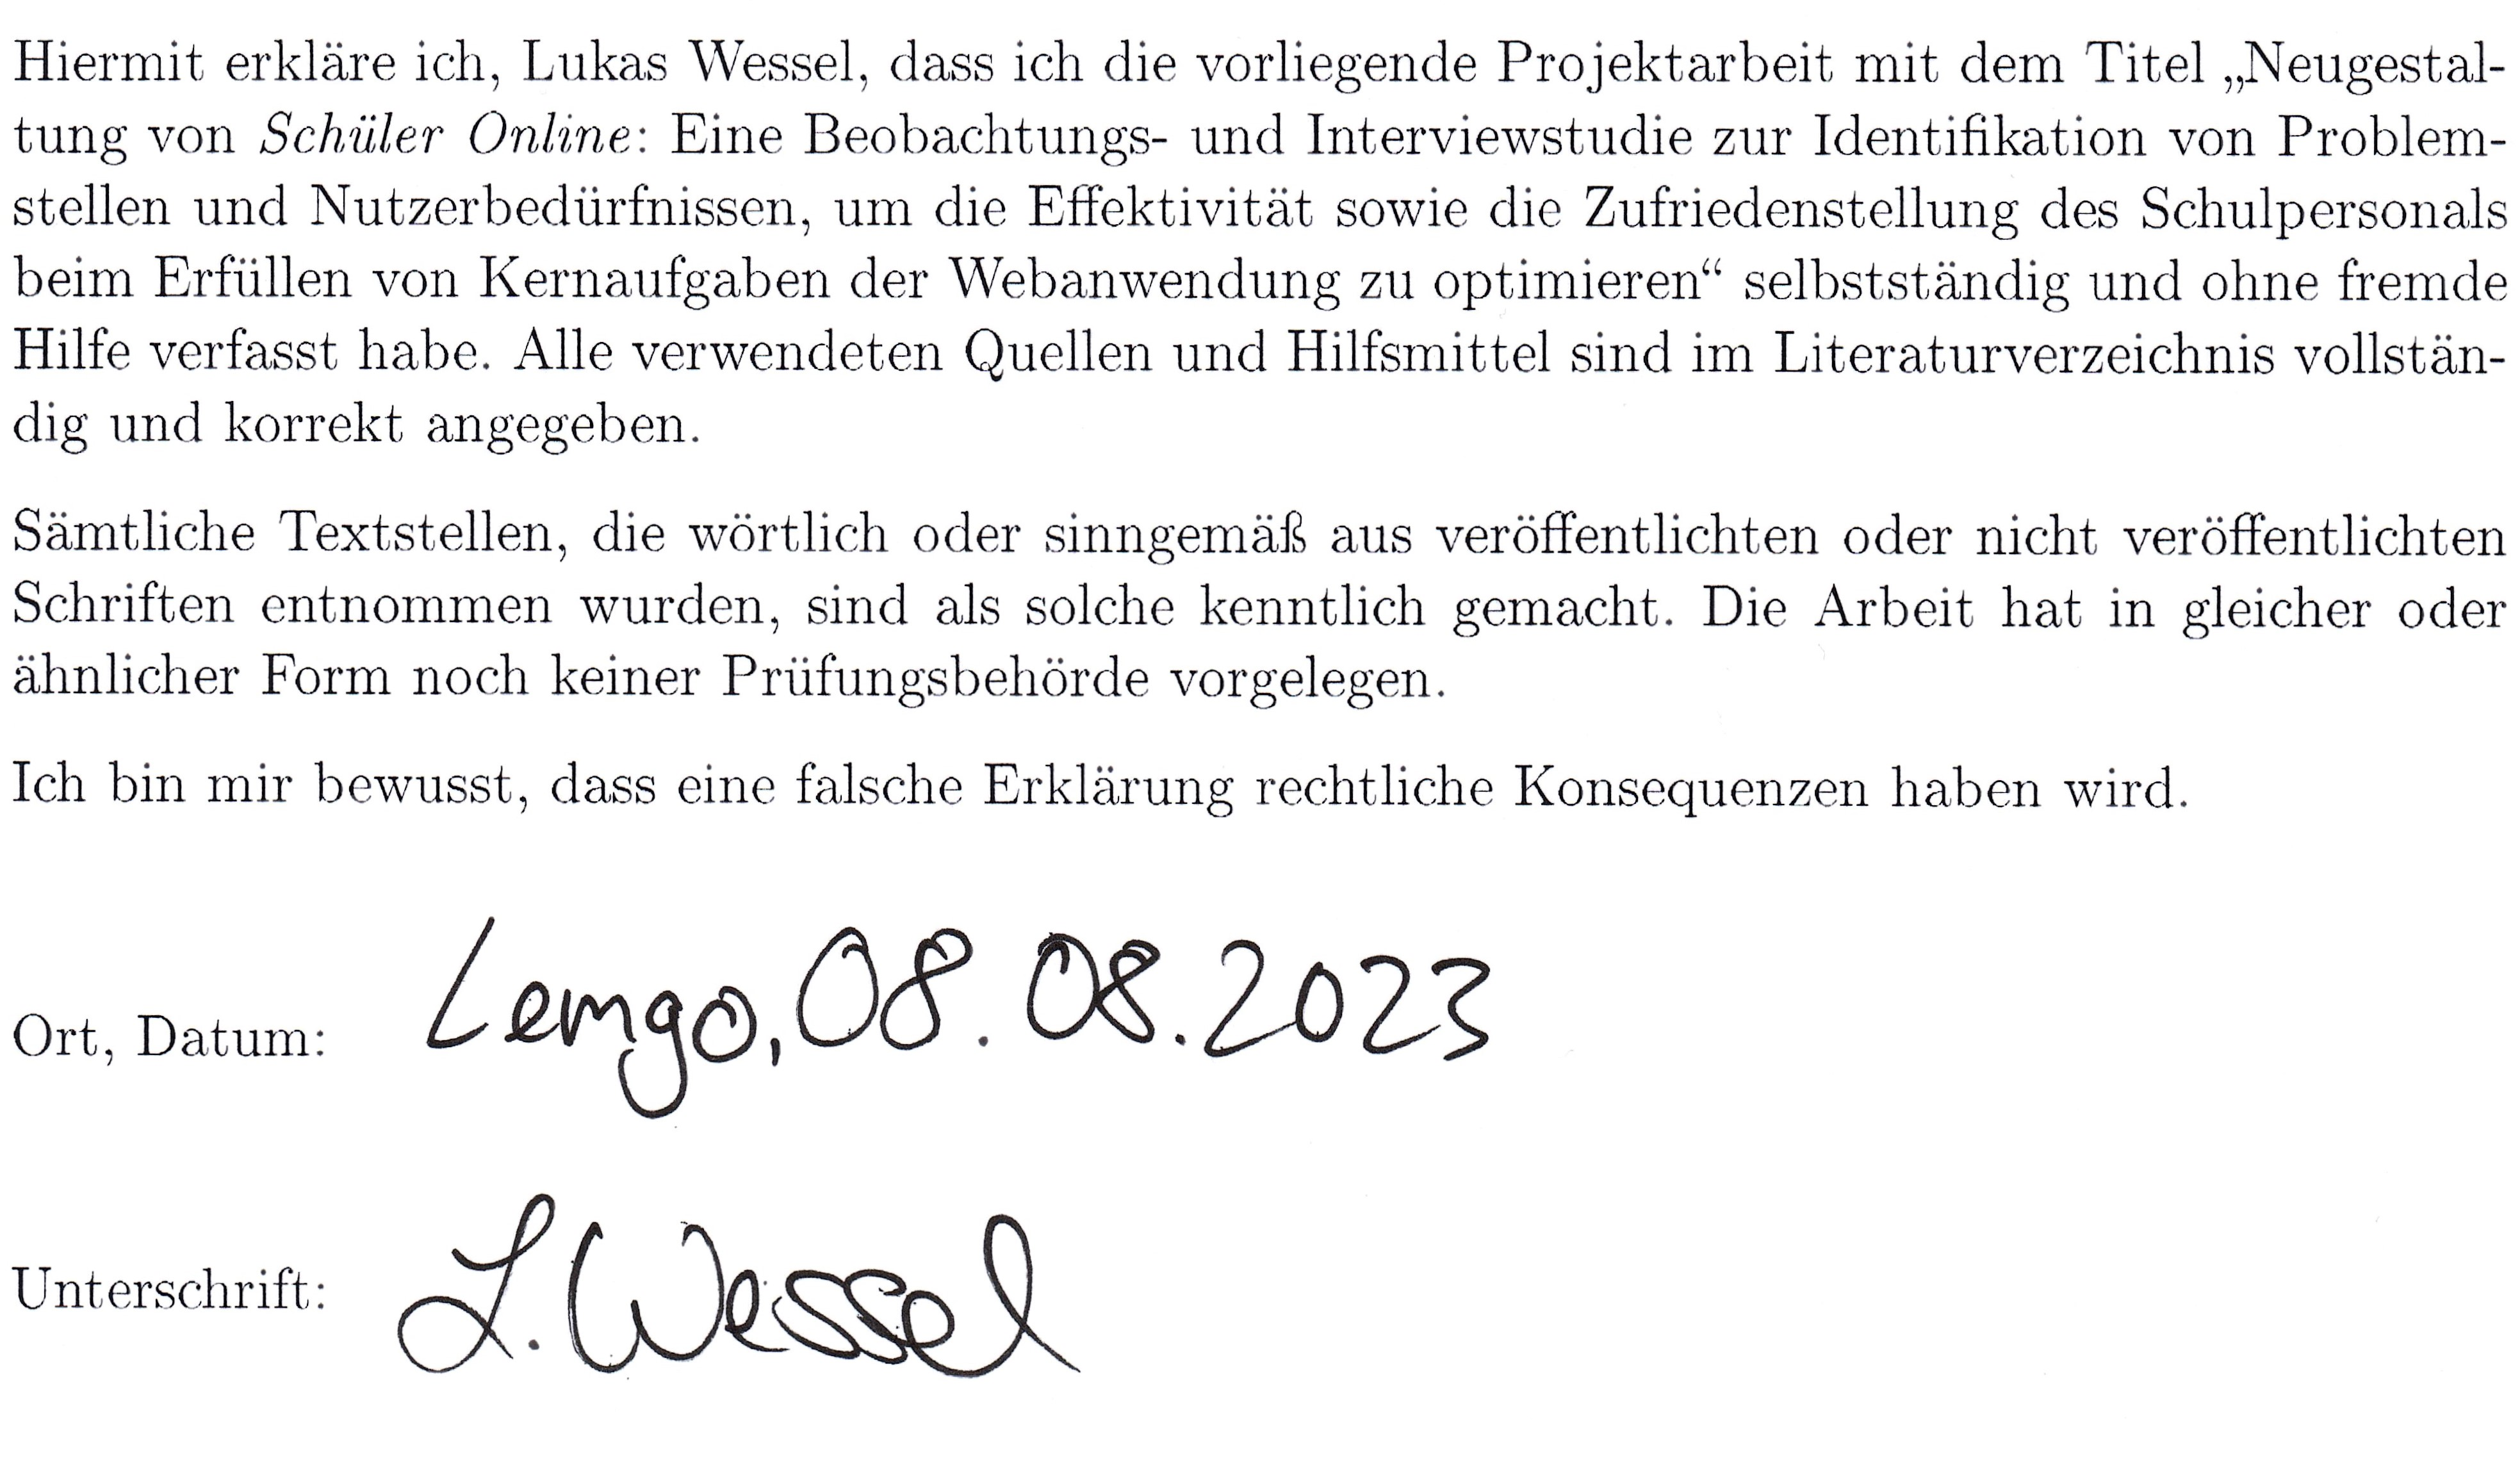
\includegraphics{eigenstaendigkeitserklaerung}
    \end{adjustbox}
\end{figure}



\newpage
\section{Anhang}

\subsection{Musteranmeldeformular}
\begin{figure}[H]
    \centering
    \caption{Musteranmeldeformular von der fiktiven Person Max Müller}
    \begin{adjustbox}{height=0.85\textheight, center}
        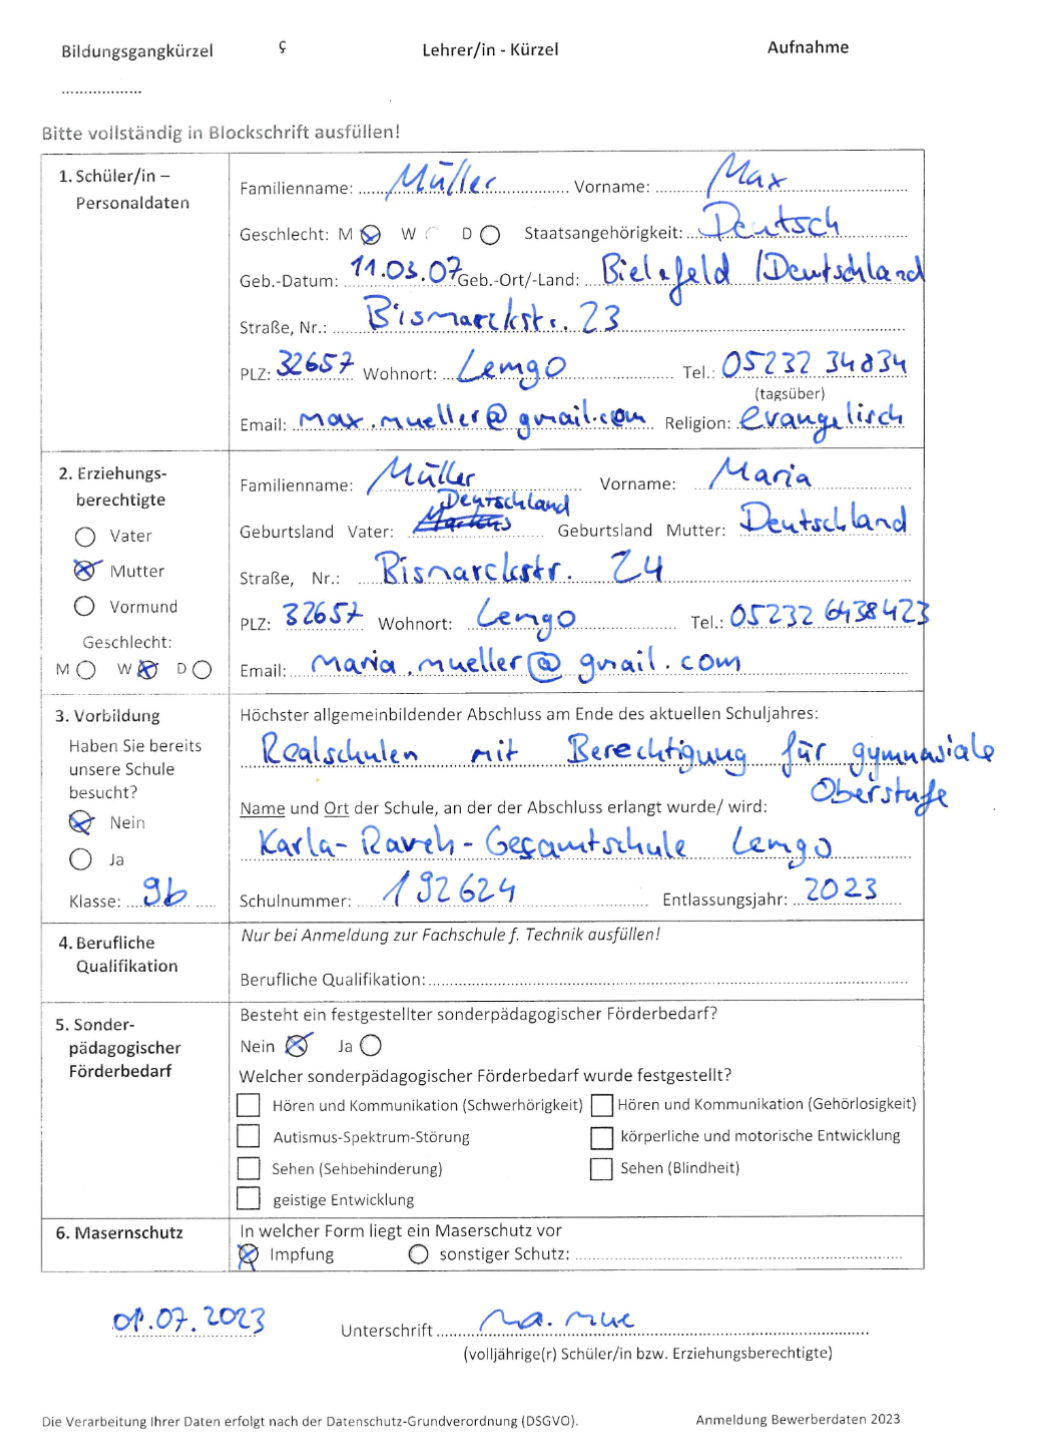
\includegraphics{bewerbungsformular1}
    \end{adjustbox}
\end{figure}

\begin{landscape}

    \begin{longtable}{p{15cm}cc}
        \caption{Your Table} \label{tab:mytable} \\
        \toprule
        Erfordernis & Beispiel & Zugehörige Ergebnisse \\
        \midrule
            Der Benutzer muss inkorrekte Daten identifizieren und korrigieren können. & a & E1, E2 \\
            Der Benutzer muss die an ihn eingereichten Formulare korrekt übertragen können. & a & E5, E6 \\
            Der Benutzer muss unzulässige Bewerbungen identifizieren können. & a & E9, E10 \\
            Der Benutzer muss die Daten datenschutzkonform in die Anwendung eintragen können und über mögliche Verstöße informiert werden. & a & E11 \\
            Der Benutzer muss erkennen können, wie er zum korrekten Prozess gelangt. & a & E12 \\
            Der Benutzer muss bezüglich Aufnahmeentscheidungen mit den Entscheidungsträgern zusammen arbeiten können. & a & E7, E8 \\
            Der Benutzer muss die Software auch bei fehlenden Daten bedienen können.  & a & \\
            Der Benutzer muss Aufnahmekriterien berücksichtigen können. & a & \\
            Der Benutzer muss Termine für Aufnahmeberatungsgespräche hinterlegen können. & a & b \\
            Der Benutzer muss Schülerakten erzeugen können. & a & b \\
            Der Benutzer muss Daten aus anderen Programmen übernehmen können. & a & b \\
            Der Benutzer muss Adressrecherchen durchführen können. & a & b \\
            Der Benutzer muss eine Kurzanleitung für den Einstieg abrufen können. & a & b \\
            Der Benutzer muss die Software auch bei fehlenden Daten bedienen können. & a & b \\
            Der Benutzer muss innerjährige Wechsel und Stufenwiederholungen erfassen können. & a & b \\
            Der Benutzer muss langfristige Beurlaubungen vermerken können. & a & b \\
            Der Benutzer muss auch komplizierte Bewerbungen und Sonderfälle bearbeiten können. & a & b \\
            Der Benutzer muss seinen bisherigen Jargon verwenden können. & a & b \\
            Der Benutzer muss die Aufgaben und Prozesse intuitiv bedienen können. & a & b \\
            Der Benutzer muss eine Adressvalidierung vornehmen können. & a & b \\
            Der Benutzer muss Erreichbarkeiten von Notfallkontakten erfassen können. & a & b \\
            Der Benutzer muss unterschiedliche Arten von Notfallkontakten erfassen können. & a & b \\
            Der Benutzer muss erkennen können, ob ein Schüler volljährig ist. & a & b \\
        \endfirsthead
        \toprule
        Erfordernis & Beispiel & Zugehörige Ergebnisse \\
        \midrule
        \endhead
        \bottomrule
        \endfoot
            Der Benutzer muss Nachweise über das Sorgerecht hinterlegen können. & a & b \\
            Der Benutzer muss Daten auch bei Programmabbrüchen wiederherstellen können. & a & b \\
            Der Benutzer muss ähnliche Datenabfragen aus vorherigen Formularen übernehmen können. & a & b \\
            Der Benutzer muss bei Bedarf Handbücher heranziehen können. & a & b \\
            Der Benutzer muss bei Bedarf Fachterminologie nachschlagen oder verstehen können. & a & b \\
            Der Benutzer muss jederzeit darüber Bescheid wissen, welche Daten den Eltern und Schülern angezeigt werden. & a & b \\
            Der Benutzer muss den Systemstatus jederzeit einsehen können. & a & b \\
            Der Benutzer muss Bewerbungslisten in geeigneter Form exportieren können. & a & b \\
            Der Benutzer muss Daten in Schulverwaltungsprogramme wie Schild exportieren können. & a & b \\
            Der Benutzer muss Daten nach Excel exportieren können. & a & b \\
            Der Benutzer muss Berichte anfertigen können. & a & b \\
            Der Benutzer muss Anmeldezeiträume berücksichtigen. & a & b \\
            Der Benutzer muss mit anderen Behörnden zusammenarbeiten können. & a & b \\
            Der Benutzer muss über Änderungen an Bewerbungen regelmäßig informiert werden. & a & b \\
            Der Benutzer muss zusätzliche Informationen zu einer Bewerbung hinterlegen können. & a & b \\
            Der Benutzer muss Dokumente ausdrücken können. & a & b \\
            Der Benutzer muss Dokumente digitalisieren und beim Datensatz hinterlegen können. & a & b \\
    \end{longtable}




\subsection{bildungsgang}
\begin{figure}[H]
    \centering
    \caption{Testüberschrift}
    \begin{adjustbox}{width=\linewidth, center}
        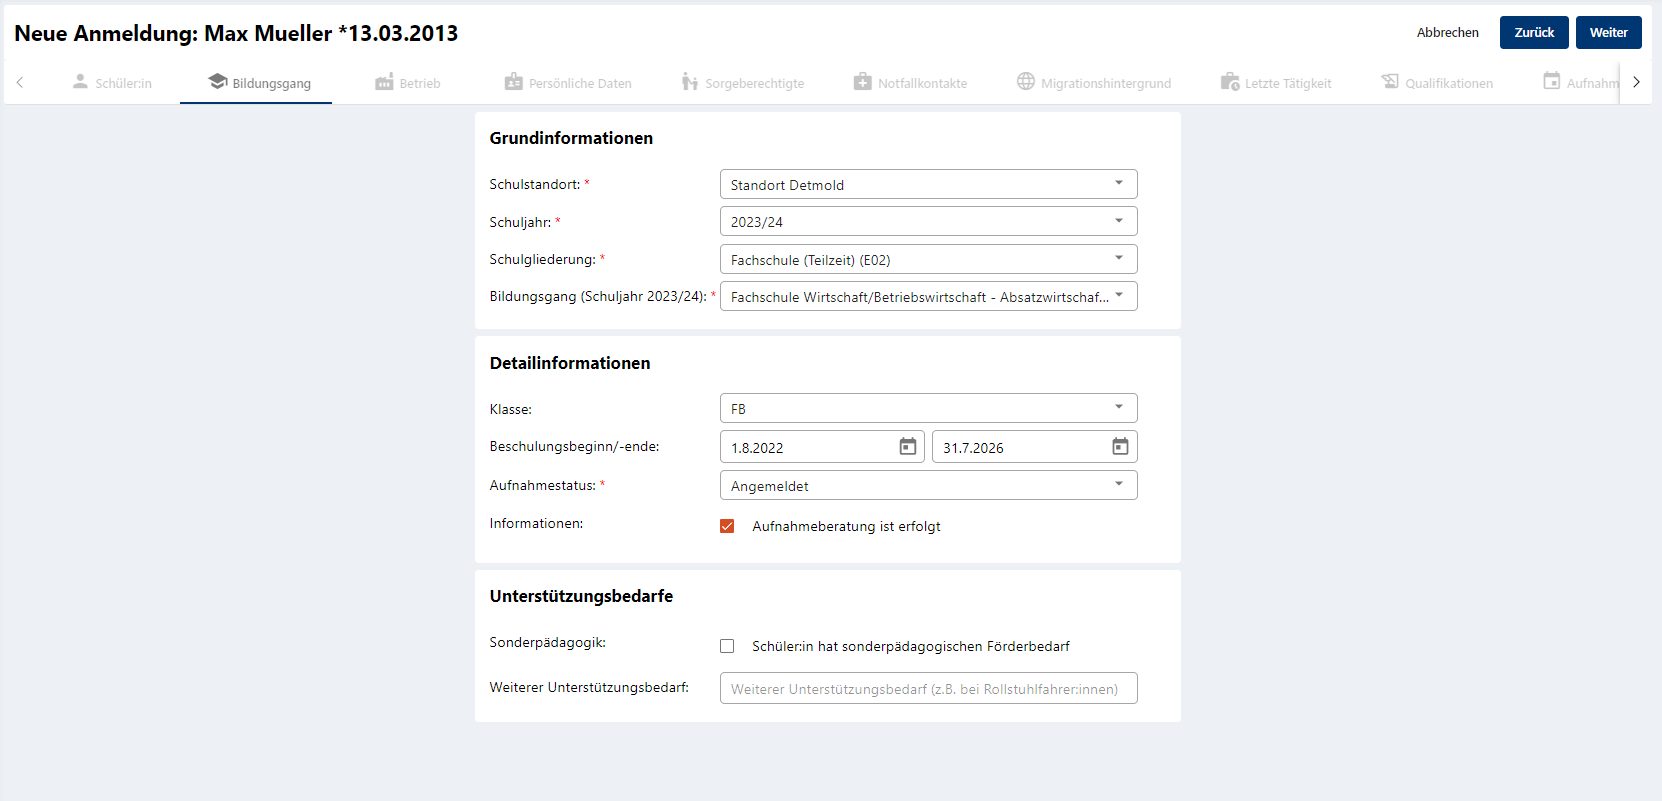
\includegraphics{bildungsgang}
    \end{adjustbox}
\end{figure}

\subsection{sorgeberechtigte-liste}
\begin{figure}[H]
    \centering
    \caption{Testüberschrift}
    \begin{adjustbox}{width=\linewidth, center}
        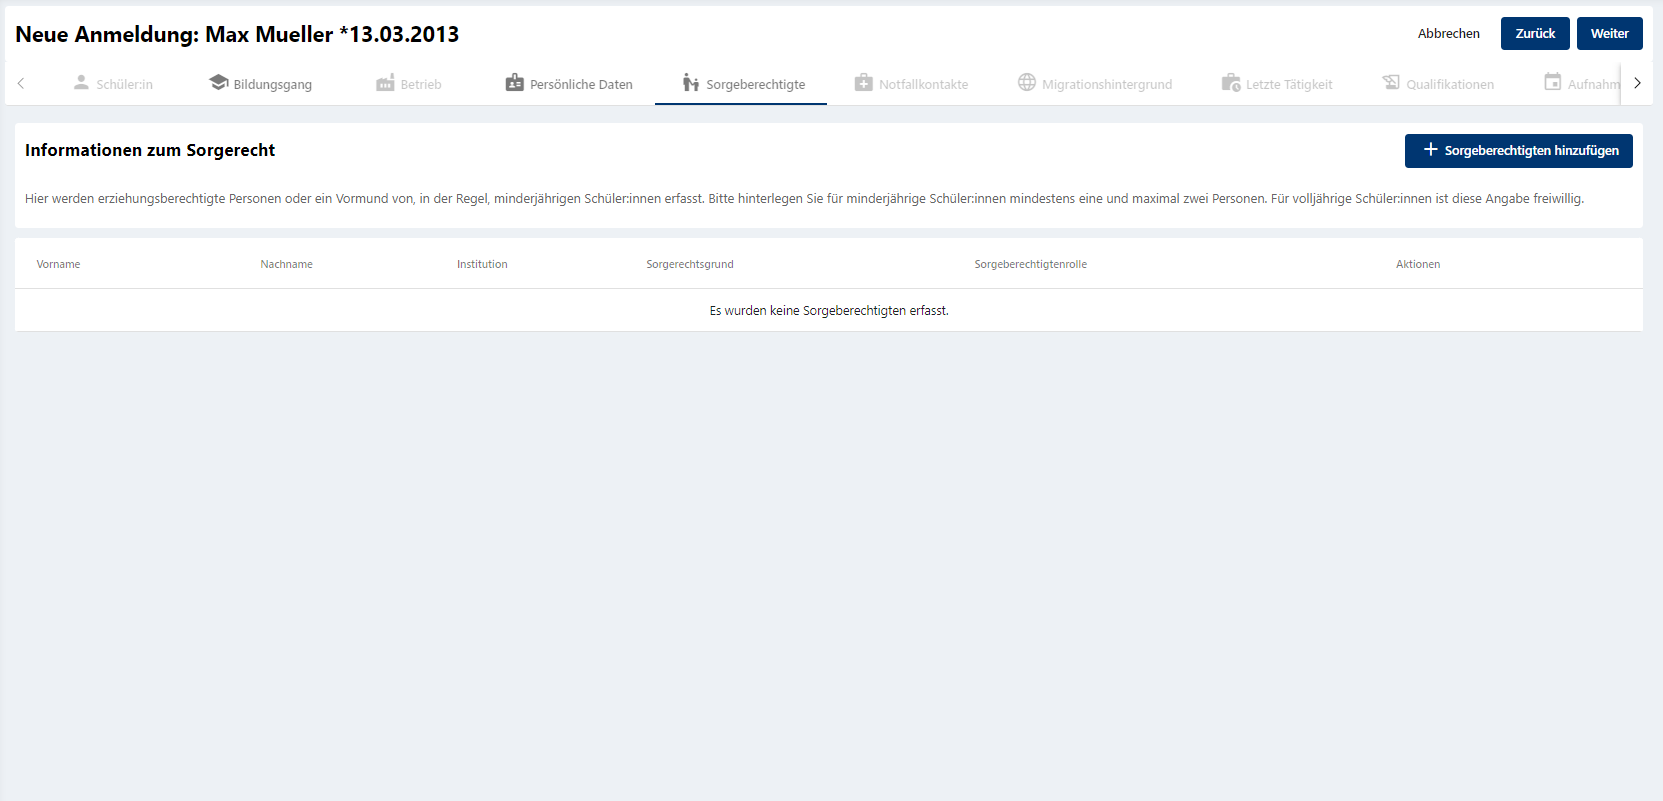
\includegraphics{sorgeberechtigte-liste}
    \end{adjustbox}
\end{figure}

\subsection{sorgeberechtigter-person}
\begin{figure}[H]
    \centering
    \caption{Testüberschrift}
    \begin{adjustbox}{width=0.5\linewidth, center}
        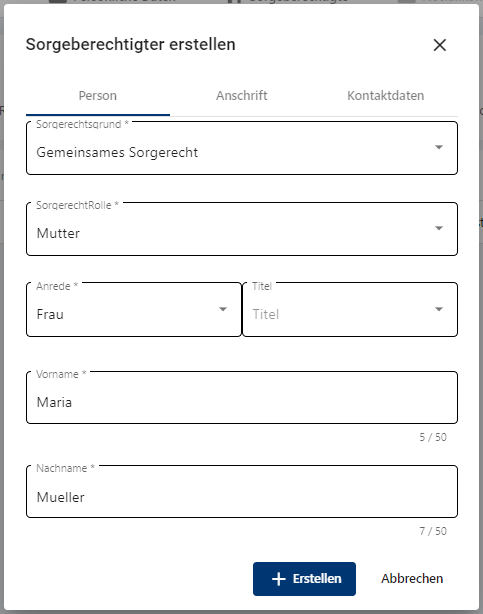
\includegraphics{sorgeberechtigter-person}
    \end{adjustbox}
\end{figure}

\subsection{sorgeberechtigter-anschrift}
\begin{figure}[H]
    \centering
    \caption{Testüberschrift}
    \begin{adjustbox}{width=0.85\linewidth, center}
        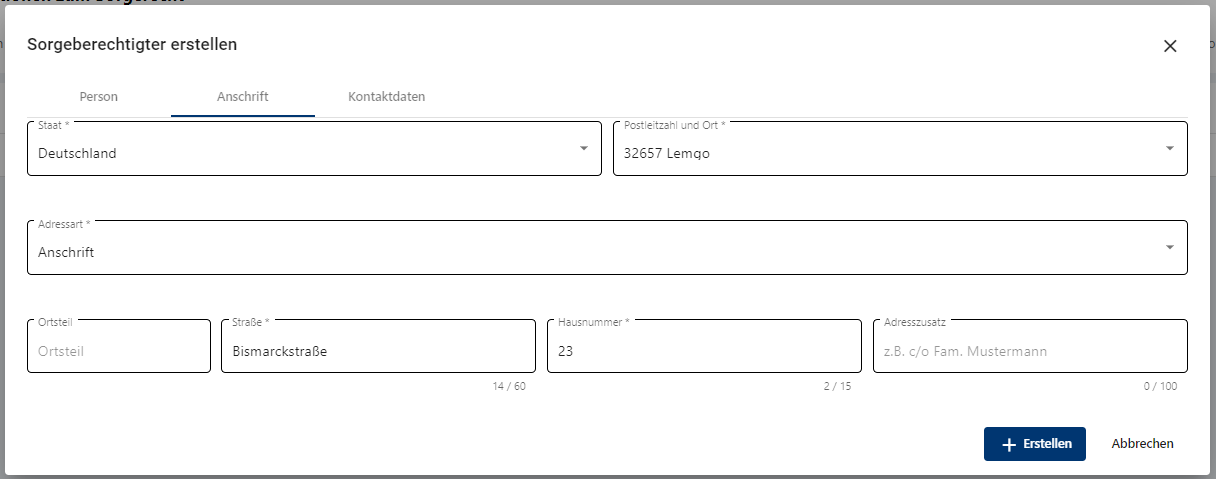
\includegraphics{sorgeberechtigter-anschrift}
    \end{adjustbox}
\end{figure}

\subsection{sorgeberechtigter-kontakt}
\begin{figure}[H]
    \centering
    \caption{Testüberschrift}
    \begin{adjustbox}{width=0.6\linewidth, center}
        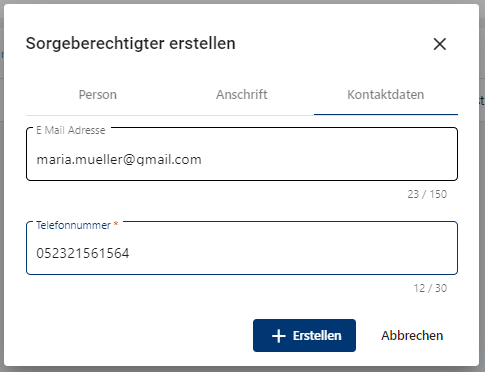
\includegraphics{sorgeberechtigter-kontakt}
    \end{adjustbox}
\end{figure}

\subsection{notfallkontakt-daten}
\begin{figure}[H]
    \centering
    \caption{Testüberschrift}
    \begin{adjustbox}{width=0.6\linewidth, center}
        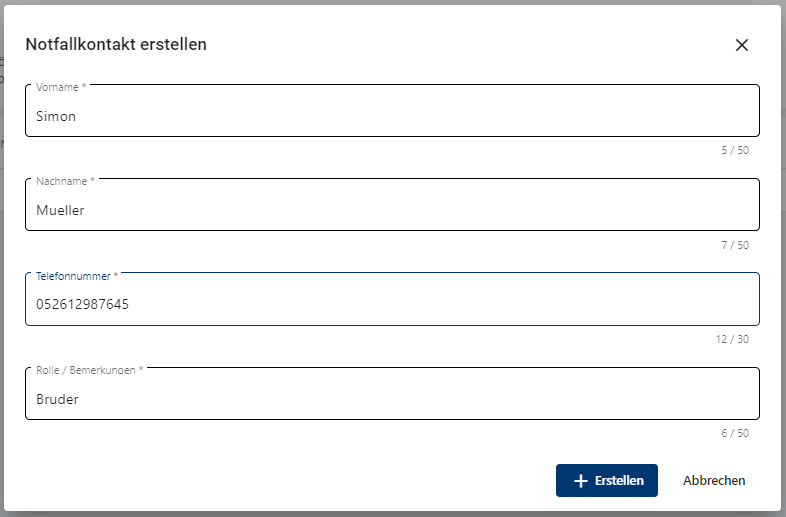
\includegraphics{notfallkontakt-daten}
    \end{adjustbox}
\end{figure}

\subsection{notfallkontakt-liste}
\begin{figure}[H]
    \centering
    \caption{Testüberschrift}
    \begin{adjustbox}{width=\linewidth, center}
        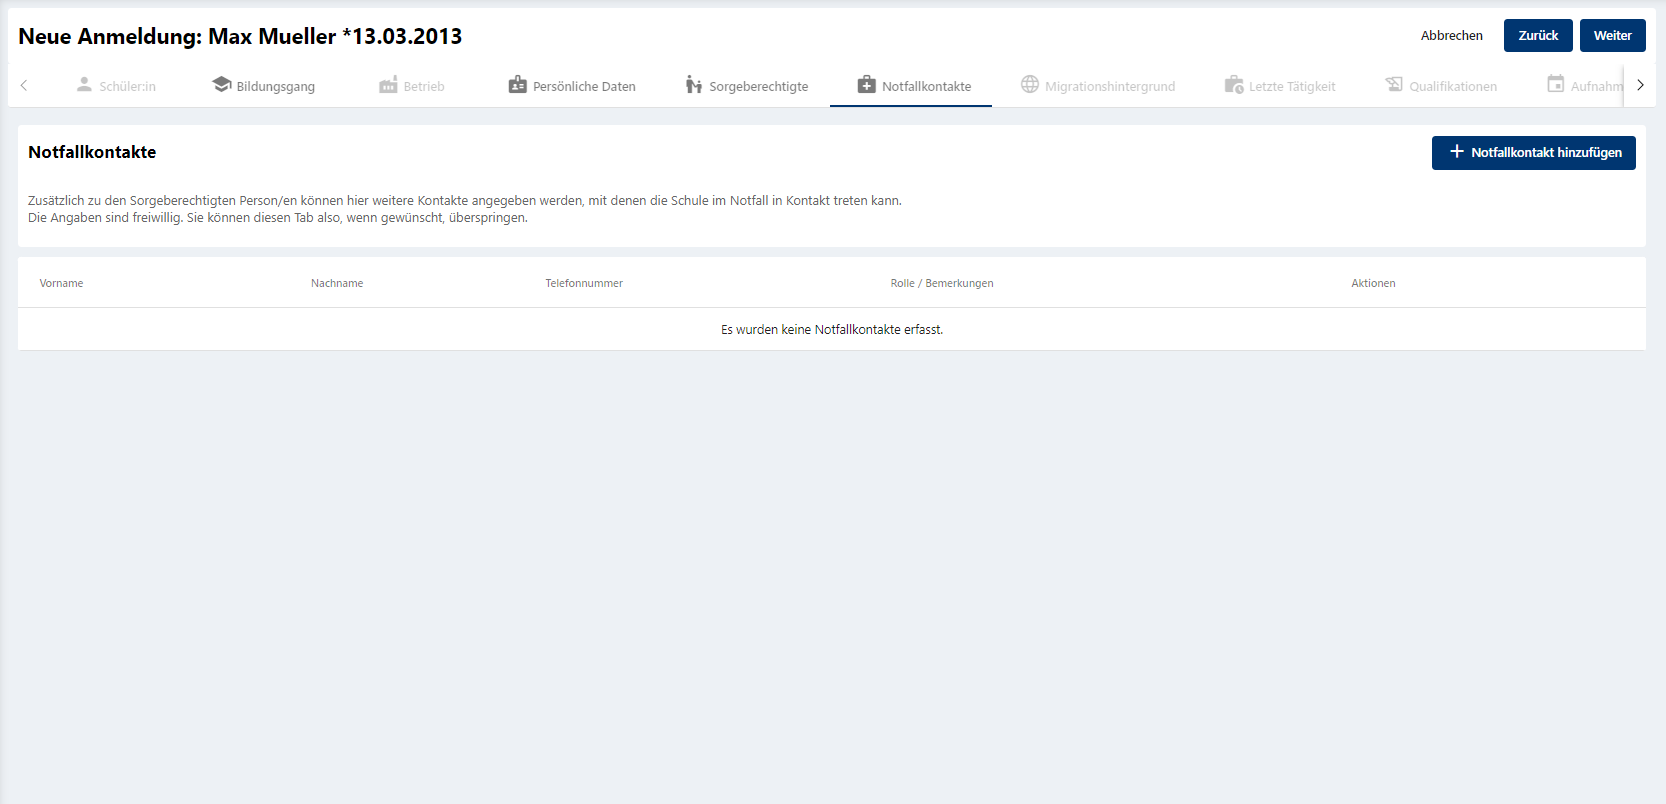
\includegraphics{notfallkontakt-liste}
    \end{adjustbox}
\end{figure}

\subsection{migrationshintergrund-liegtvor}
\begin{figure}[H]
    \centering
    \caption{Testüberschrift}
    \begin{adjustbox}{width=\linewidth, center}
        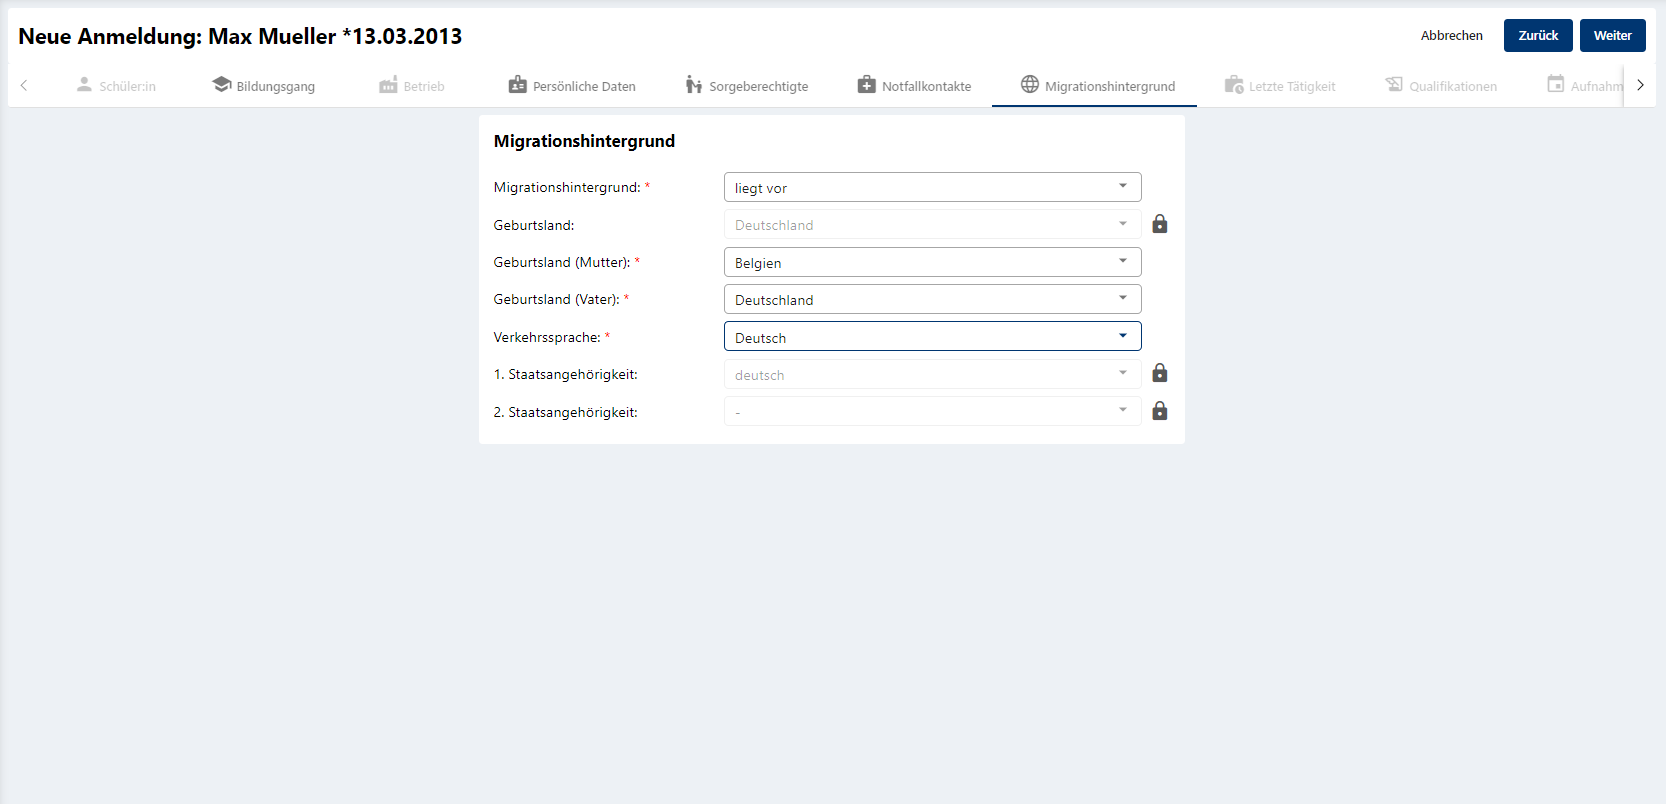
\includegraphics{migrationshintergrund-liegtvor}
    \end{adjustbox}
\end{figure}

\subsection{migrationshintergrund-liegtnichtvor}
\begin{figure}[H]
    \centering
    \caption{Testüberschrift}
    \begin{adjustbox}{width=\linewidth, center}
        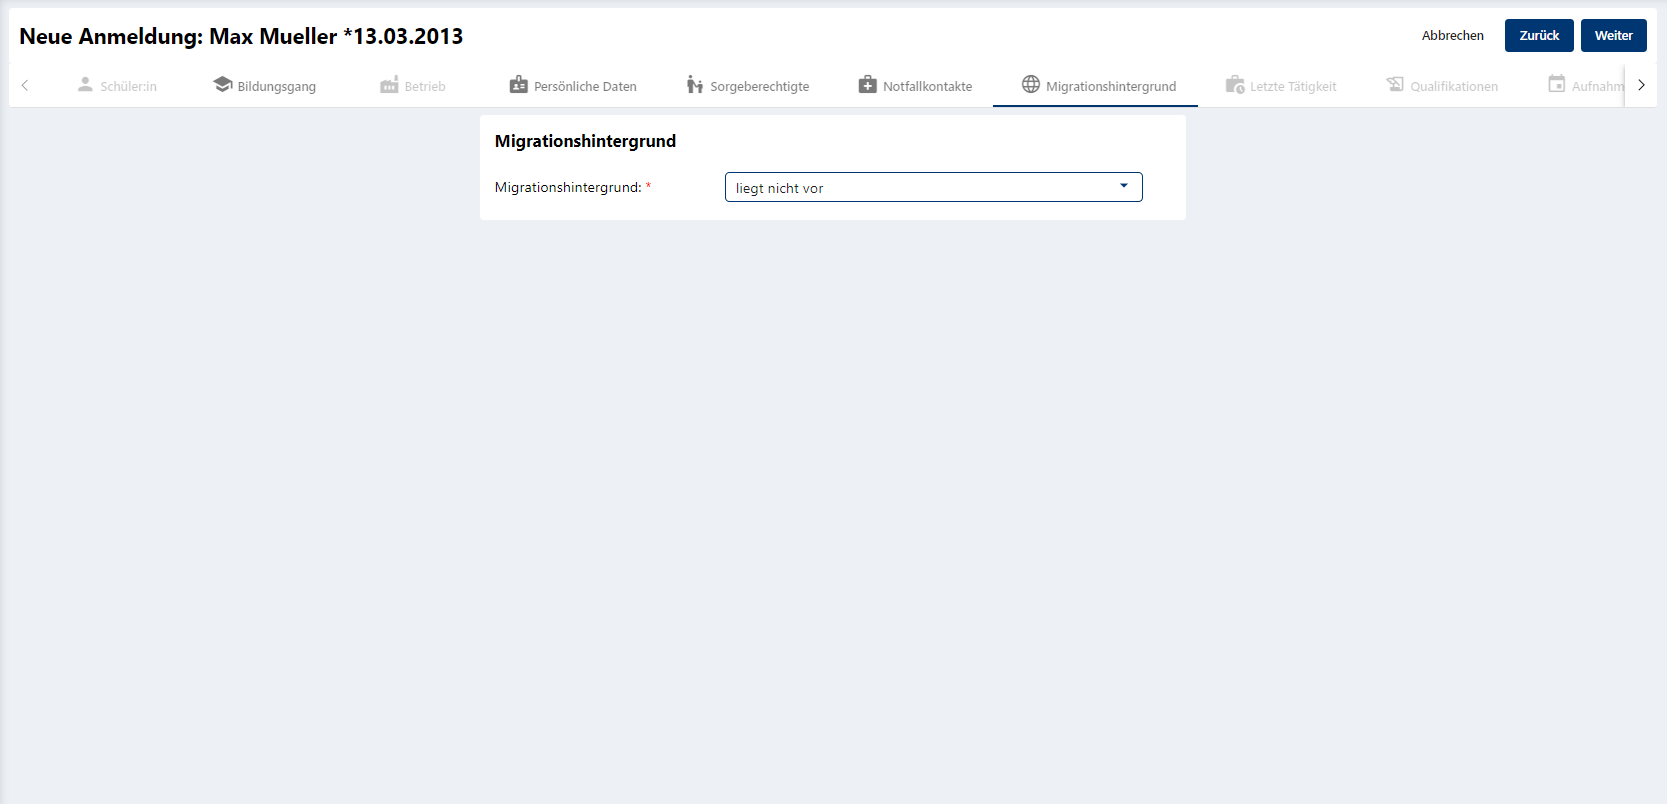
\includegraphics{migrationshintergrund-liegtnichtvor}
    \end{adjustbox}
\end{figure}

\subsection{qualifikation}
\begin{figure}[H]
    \centering
    \caption{Testüberschrift}
    \begin{adjustbox}{width=\linewidth, center}
        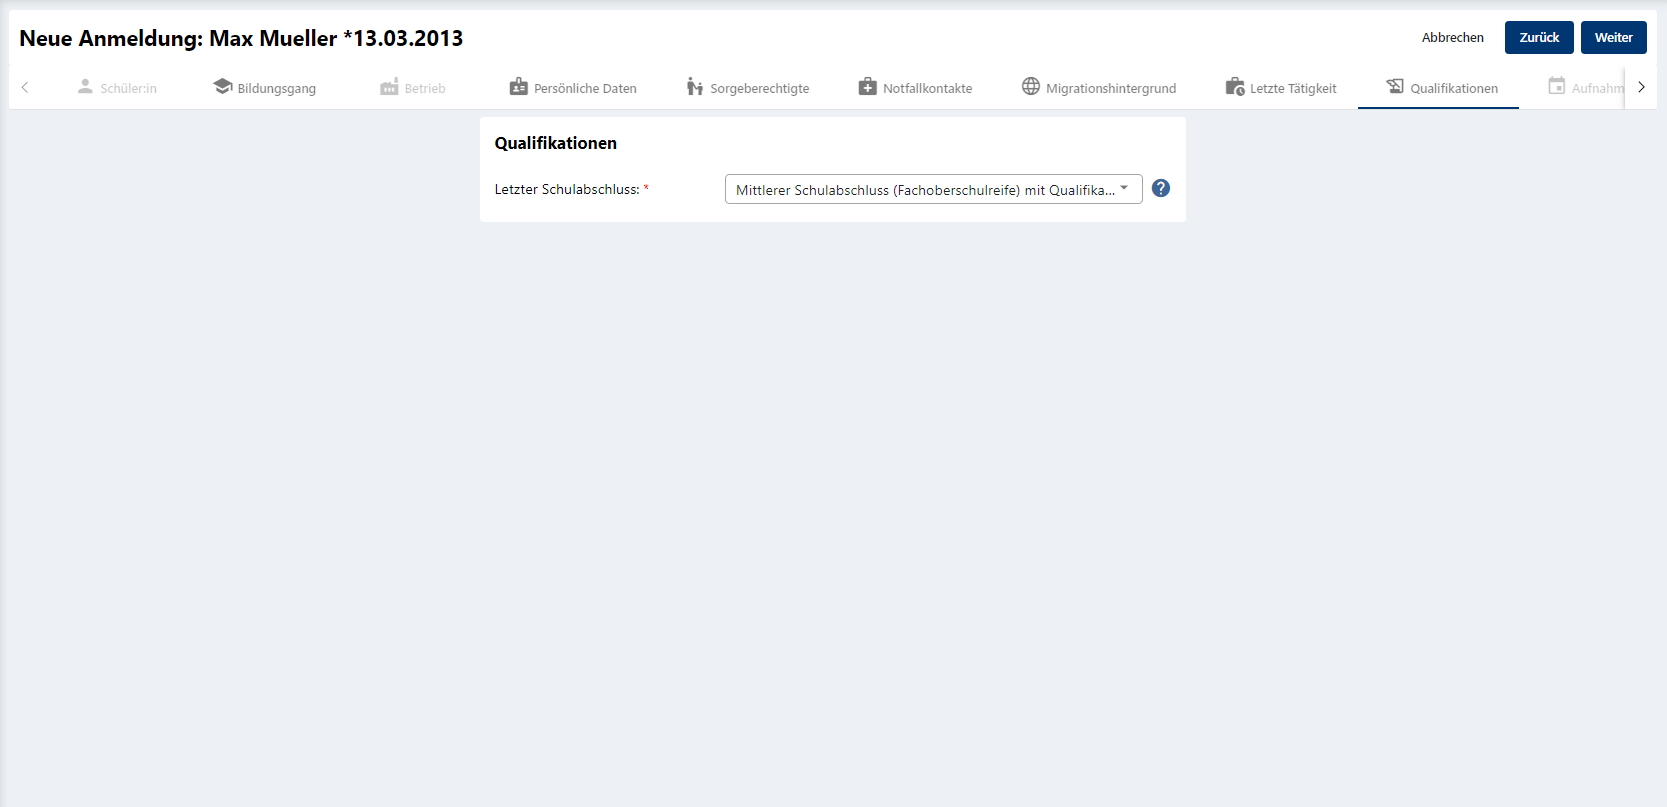
\includegraphics{qualifikation}
    \end{adjustbox}
\end{figure}

\subsection{letztetaetigkeit}
\begin{figure}[H]
    \centering
    \caption{Testüberschrift}
    \begin{adjustbox}{width=\linewidth, center}
        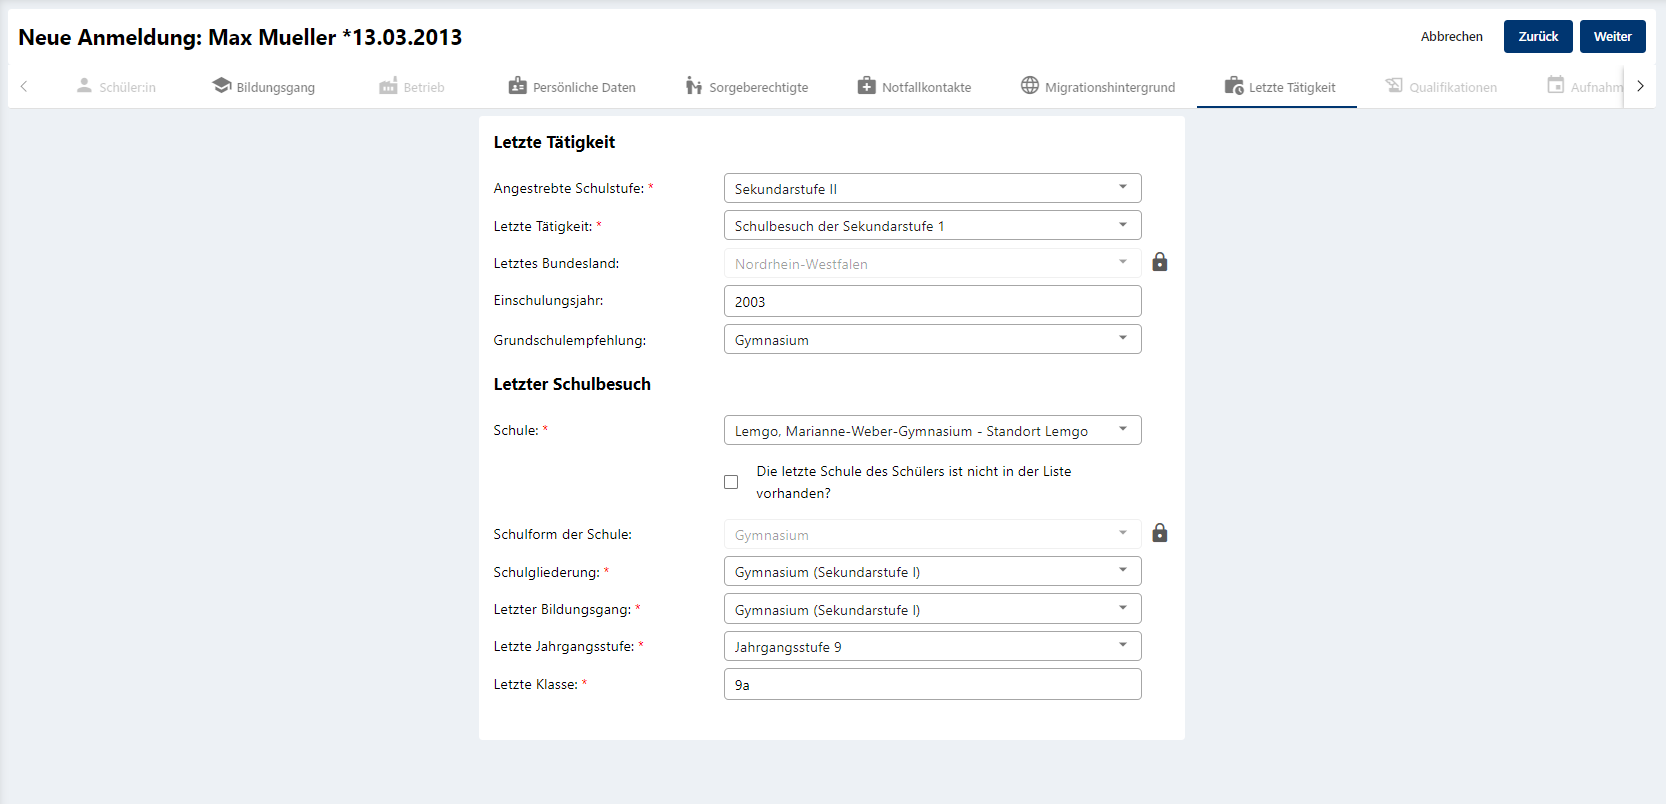
\includegraphics{letztetaetigkeit}
    \end{adjustbox}
\end{figure}

\subsection{aufnahmeberatung}
\begin{figure}[H]
    \centering
    \caption{Testüberschrift}
    \begin{adjustbox}{width=\linewidth, center}
        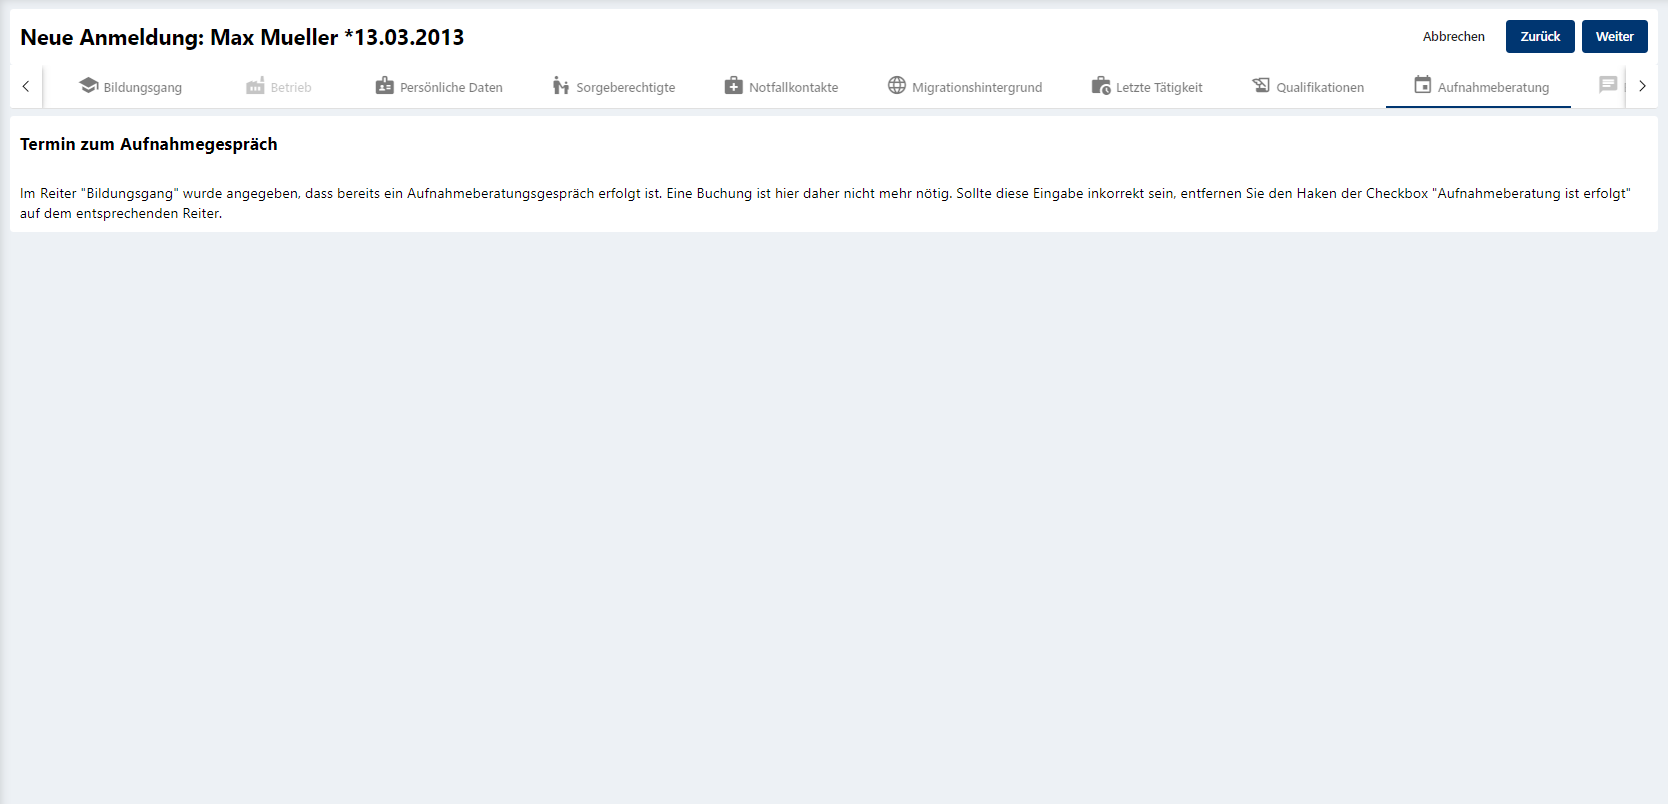
\includegraphics{aufnahmeberatung}
    \end{adjustbox}
\end{figure}

\subsection{bemerkungen}
\begin{figure}[H]
    \centering
    \caption{Testüberschrift}
    \begin{adjustbox}{width=\linewidth, center}
        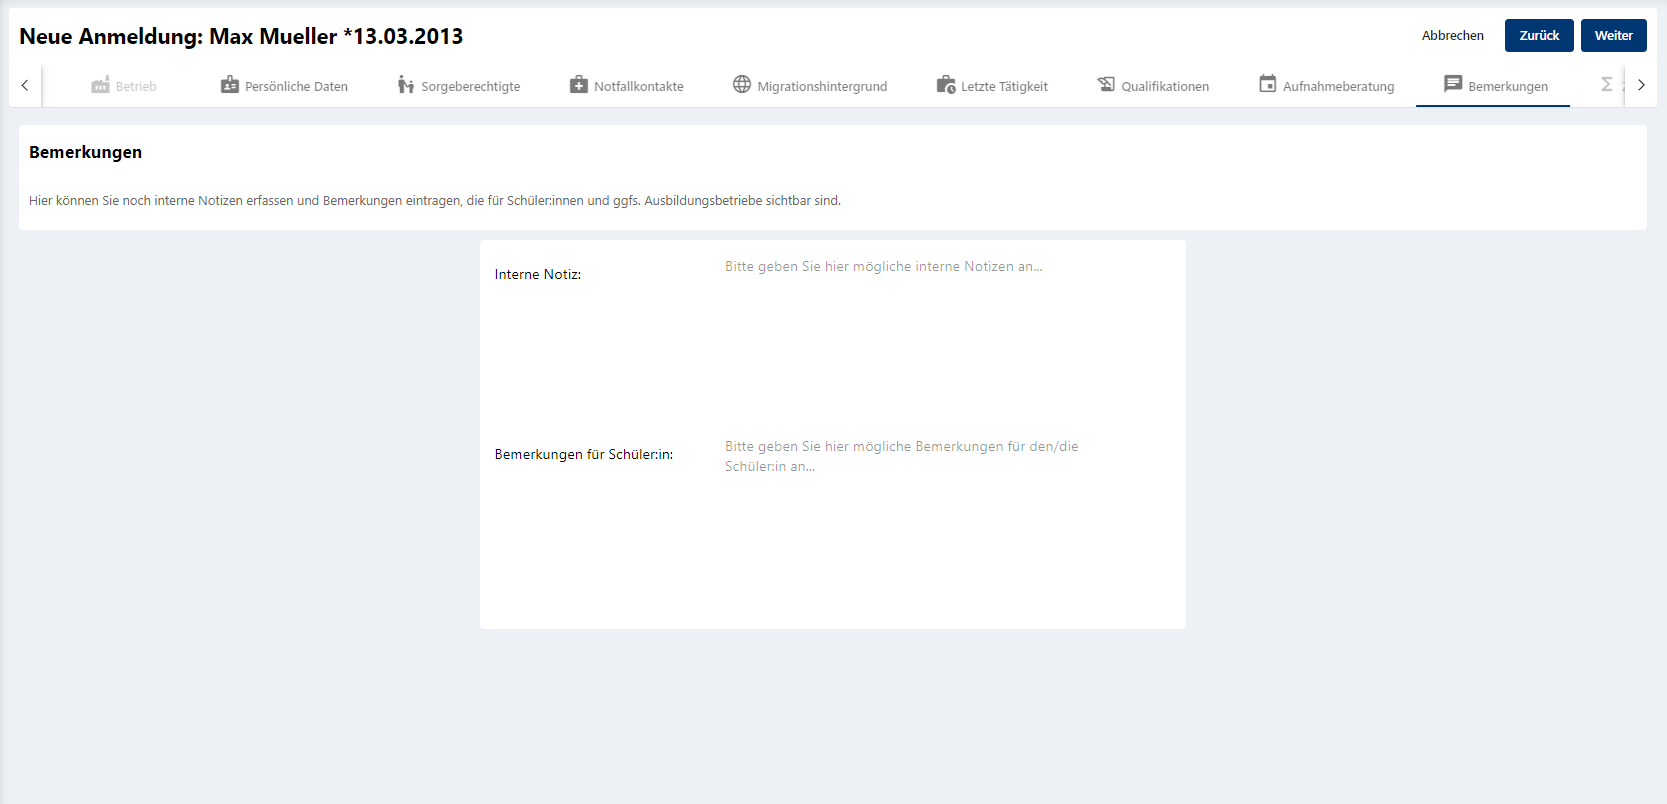
\includegraphics{bemerkungen}
    \end{adjustbox}
\end{figure}

\subsection{zusammenfassung}
\begin{figure}[H]
    \centering
    \caption{Testüberschrift}
    \begin{adjustbox}{width=\linewidth, center}
        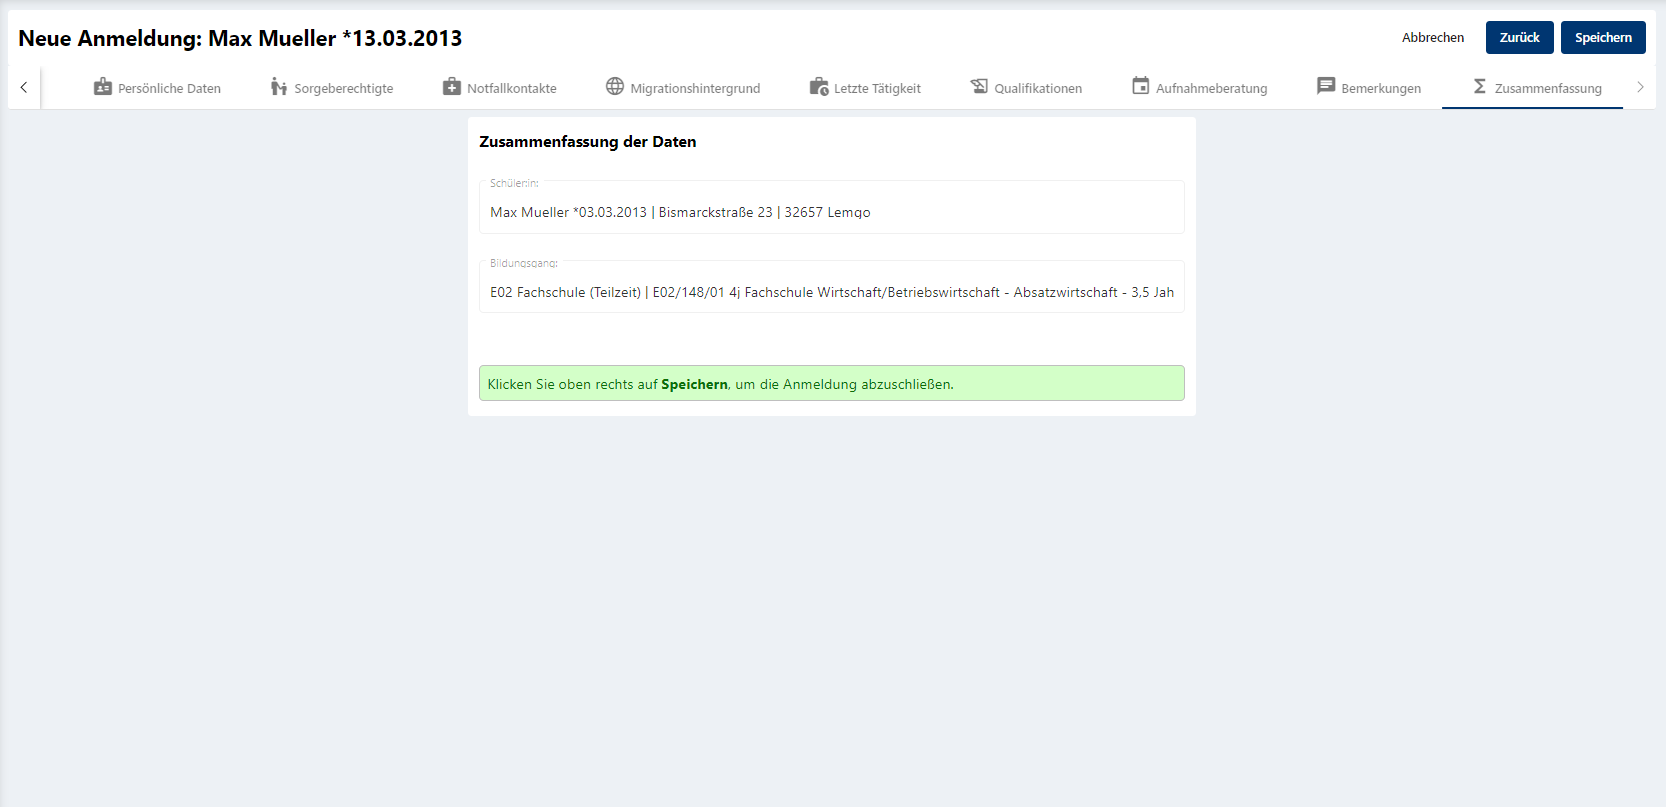
\includegraphics{zusammenfassung}
    \end{adjustbox}
\end{figure}

\subsection{bestaetigung}
\begin{figure}[H]
    \centering
    \caption{Testüberschrift}
    \begin{adjustbox}{width=\linewidth, center}
        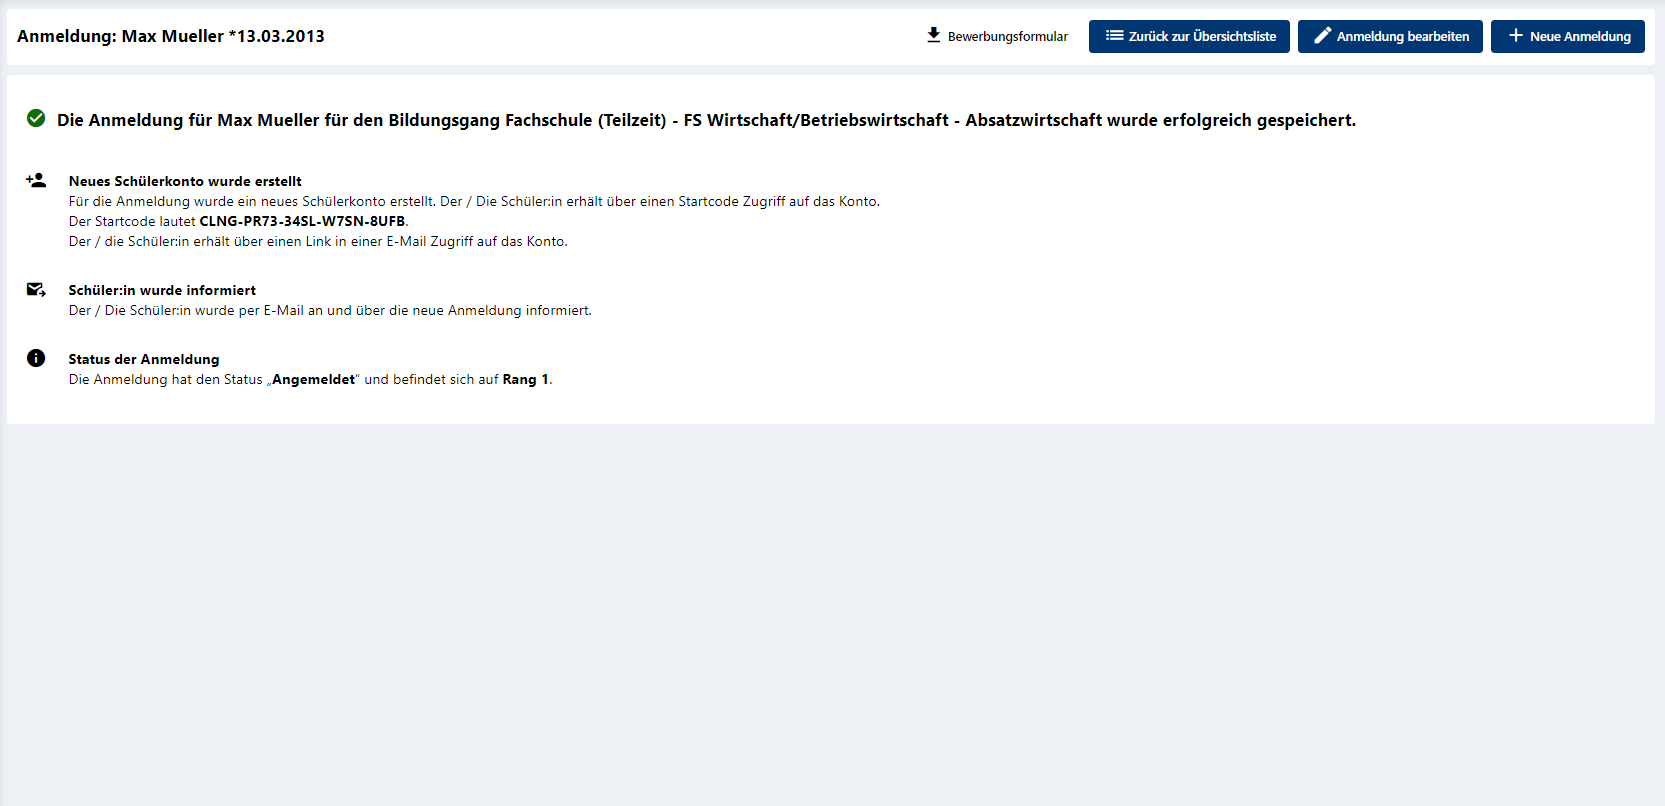
\includegraphics{bestaetigung}
    \end{adjustbox}
\end{figure}

\subsection{update-bewerbung}
\begin{figure}[H]
    \centering
    \caption{Testüberschrift}
    \begin{adjustbox}{width=\linewidth, center}
        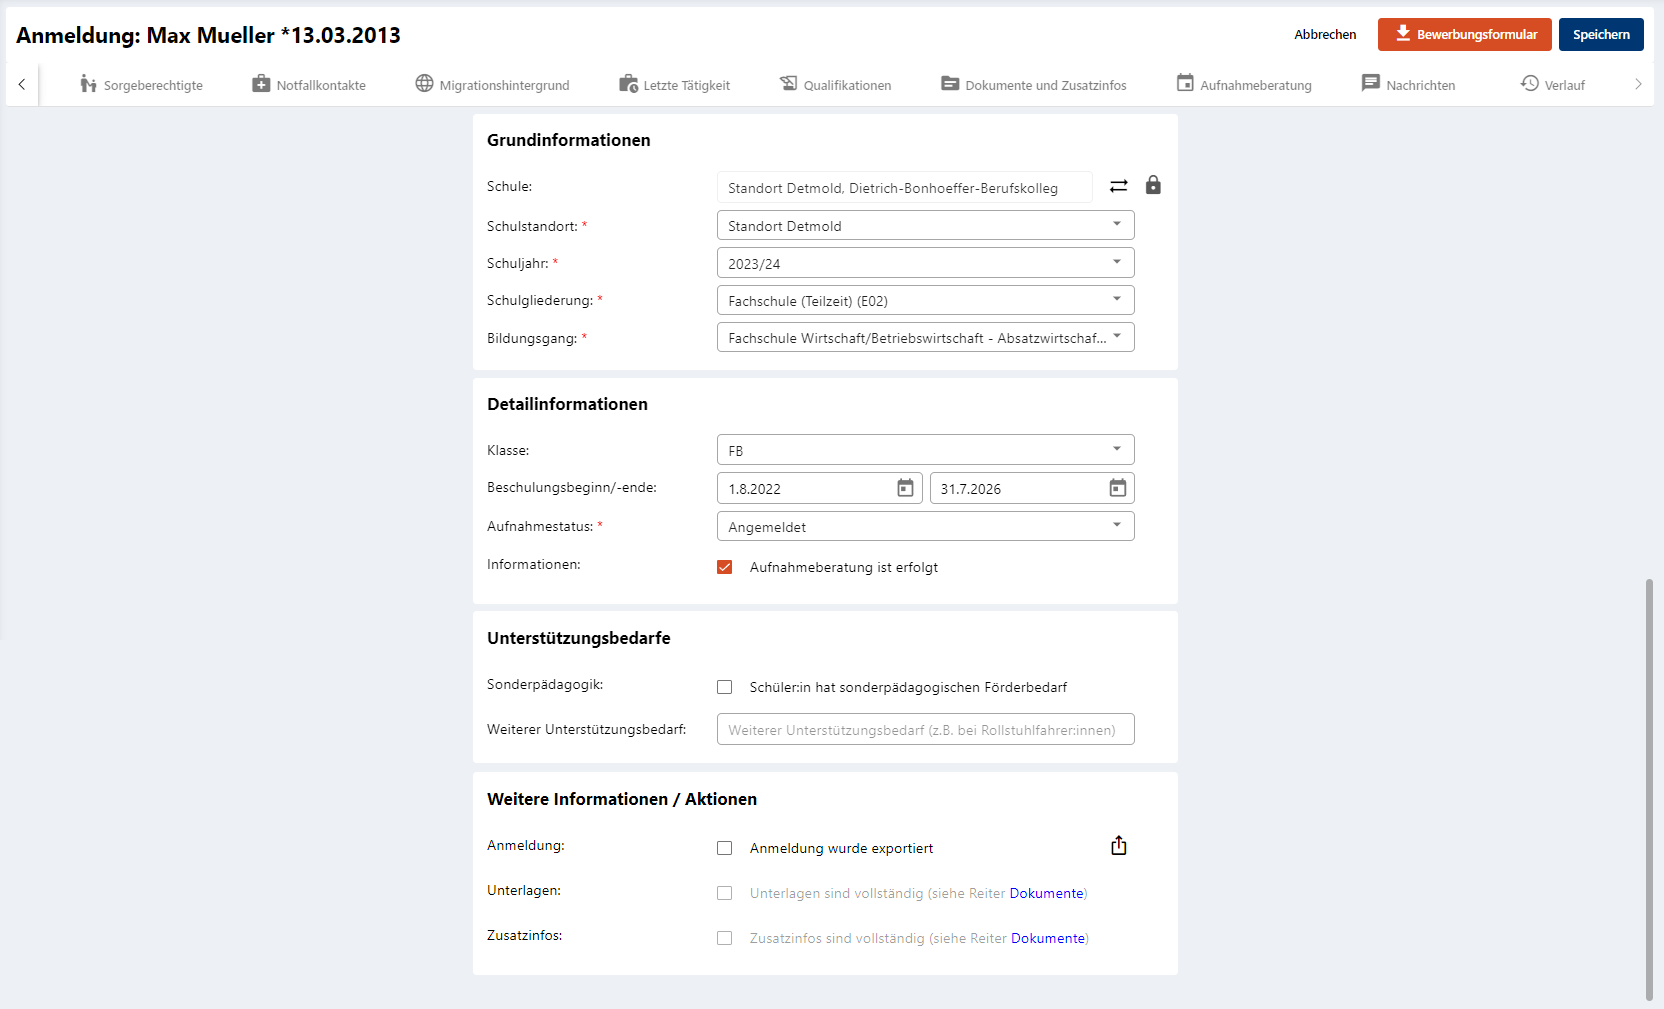
\includegraphics{update-bewerbung}
    \end{adjustbox}
\end{figure}

\end{landscape}


%\appendix
%
\newpage
\section{Anhang}

\subsection{Musteranmeldeformular}
\begin{figure}[H]
    \centering
    \caption{Musteranmeldeformular von der fiktiven Person Max Müller}
    \begin{adjustbox}{height=0.85\textheight, center}
        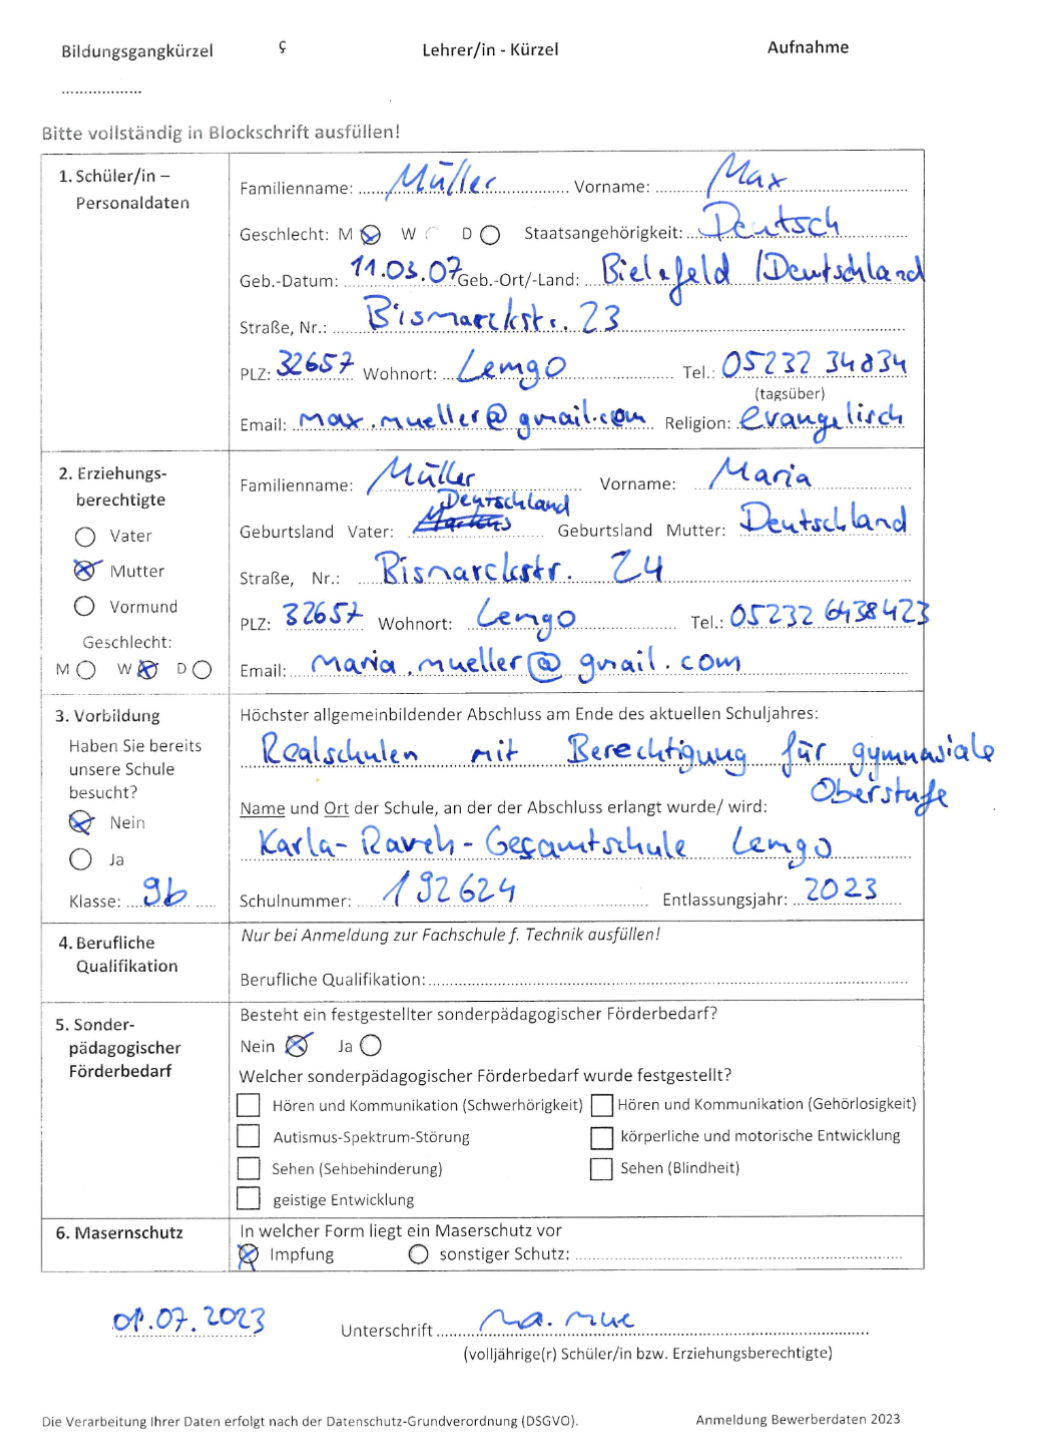
\includegraphics{bewerbungsformular1}
    \end{adjustbox}
\end{figure}

\begin{landscape}

    \begin{longtable}{p{15cm}cc}
        \caption{Your Table} \label{tab:mytable} \\
        \toprule
        Erfordernis & Beispiel & Zugehörige Ergebnisse \\
        \midrule
            Der Benutzer muss inkorrekte Daten identifizieren und korrigieren können. & a & E1, E2 \\
            Der Benutzer muss die an ihn eingereichten Formulare korrekt übertragen können. & a & E5, E6 \\
            Der Benutzer muss unzulässige Bewerbungen identifizieren können. & a & E9, E10 \\
            Der Benutzer muss die Daten datenschutzkonform in die Anwendung eintragen können und über mögliche Verstöße informiert werden. & a & E11 \\
            Der Benutzer muss erkennen können, wie er zum korrekten Prozess gelangt. & a & E12 \\
            Der Benutzer muss bezüglich Aufnahmeentscheidungen mit den Entscheidungsträgern zusammen arbeiten können. & a & E7, E8 \\
            Der Benutzer muss die Software auch bei fehlenden Daten bedienen können.  & a & \\
            Der Benutzer muss Aufnahmekriterien berücksichtigen können. & a & \\
            Der Benutzer muss Termine für Aufnahmeberatungsgespräche hinterlegen können. & a & b \\
            Der Benutzer muss Schülerakten erzeugen können. & a & b \\
            Der Benutzer muss Daten aus anderen Programmen übernehmen können. & a & b \\
            Der Benutzer muss Adressrecherchen durchführen können. & a & b \\
            Der Benutzer muss eine Kurzanleitung für den Einstieg abrufen können. & a & b \\
            Der Benutzer muss die Software auch bei fehlenden Daten bedienen können. & a & b \\
            Der Benutzer muss innerjährige Wechsel und Stufenwiederholungen erfassen können. & a & b \\
            Der Benutzer muss langfristige Beurlaubungen vermerken können. & a & b \\
            Der Benutzer muss auch komplizierte Bewerbungen und Sonderfälle bearbeiten können. & a & b \\
            Der Benutzer muss seinen bisherigen Jargon verwenden können. & a & b \\
            Der Benutzer muss die Aufgaben und Prozesse intuitiv bedienen können. & a & b \\
            Der Benutzer muss eine Adressvalidierung vornehmen können. & a & b \\
            Der Benutzer muss Erreichbarkeiten von Notfallkontakten erfassen können. & a & b \\
            Der Benutzer muss unterschiedliche Arten von Notfallkontakten erfassen können. & a & b \\
            Der Benutzer muss erkennen können, ob ein Schüler volljährig ist. & a & b \\
        \endfirsthead
        \toprule
        Erfordernis & Beispiel & Zugehörige Ergebnisse \\
        \midrule
        \endhead
        \bottomrule
        \endfoot
            Der Benutzer muss Nachweise über das Sorgerecht hinterlegen können. & a & b \\
            Der Benutzer muss Daten auch bei Programmabbrüchen wiederherstellen können. & a & b \\
            Der Benutzer muss ähnliche Datenabfragen aus vorherigen Formularen übernehmen können. & a & b \\
            Der Benutzer muss bei Bedarf Handbücher heranziehen können. & a & b \\
            Der Benutzer muss bei Bedarf Fachterminologie nachschlagen oder verstehen können. & a & b \\
            Der Benutzer muss jederzeit darüber Bescheid wissen, welche Daten den Eltern und Schülern angezeigt werden. & a & b \\
            Der Benutzer muss den Systemstatus jederzeit einsehen können. & a & b \\
            Der Benutzer muss Bewerbungslisten in geeigneter Form exportieren können. & a & b \\
            Der Benutzer muss Daten in Schulverwaltungsprogramme wie Schild exportieren können. & a & b \\
            Der Benutzer muss Daten nach Excel exportieren können. & a & b \\
            Der Benutzer muss Berichte anfertigen können. & a & b \\
            Der Benutzer muss Anmeldezeiträume berücksichtigen. & a & b \\
            Der Benutzer muss mit anderen Behörnden zusammenarbeiten können. & a & b \\
            Der Benutzer muss über Änderungen an Bewerbungen regelmäßig informiert werden. & a & b \\
            Der Benutzer muss zusätzliche Informationen zu einer Bewerbung hinterlegen können. & a & b \\
            Der Benutzer muss Dokumente ausdrücken können. & a & b \\
            Der Benutzer muss Dokumente digitalisieren und beim Datensatz hinterlegen können. & a & b \\
    \end{longtable}




\subsection{bildungsgang}
\begin{figure}[H]
    \centering
    \caption{Testüberschrift}
    \begin{adjustbox}{width=\linewidth, center}
        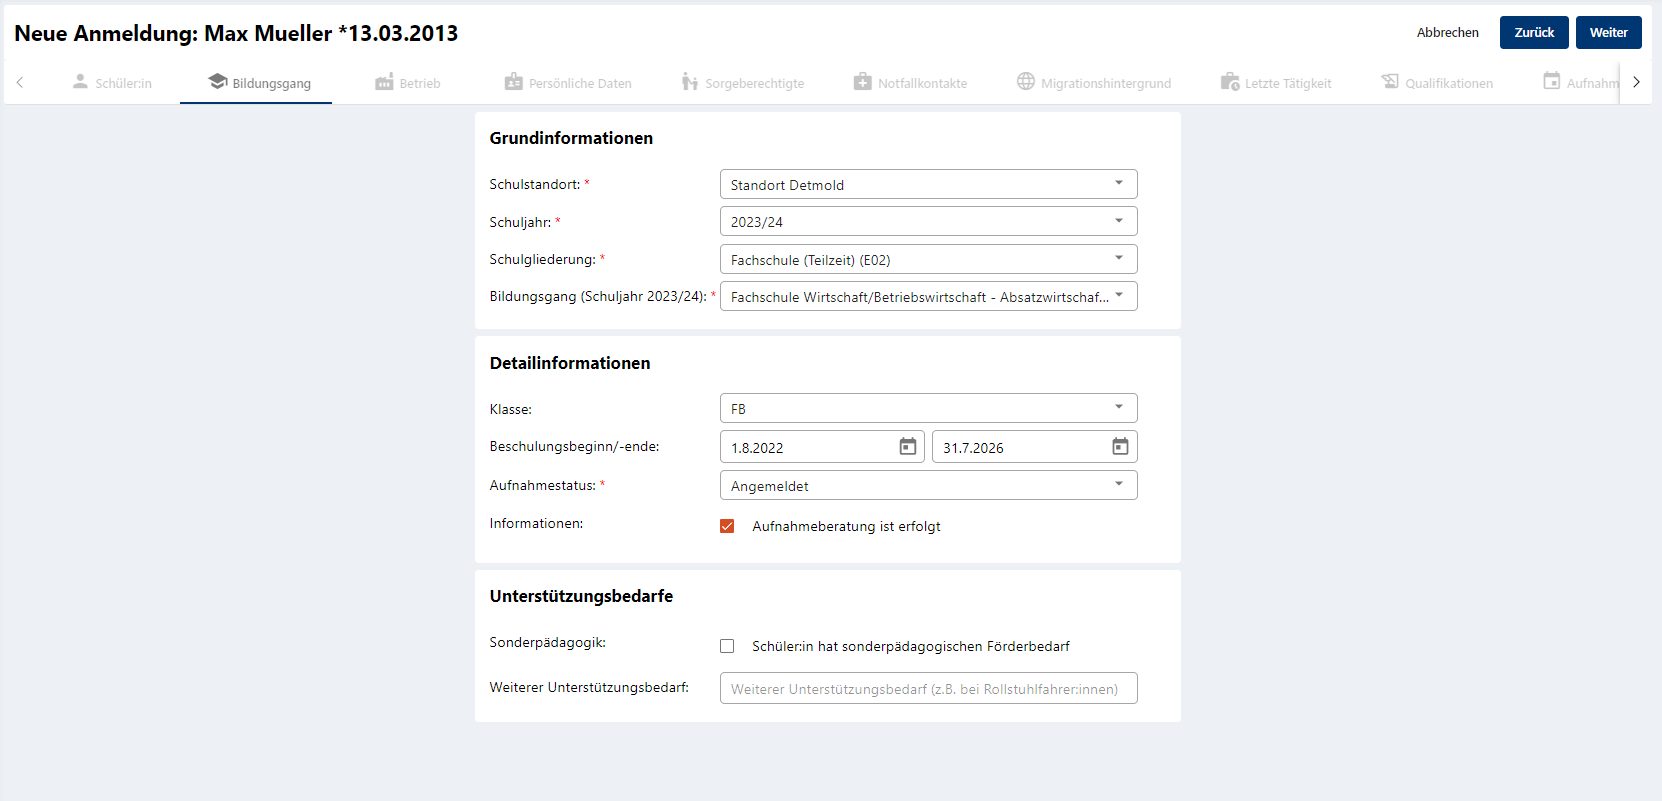
\includegraphics{bildungsgang}
    \end{adjustbox}
\end{figure}

\subsection{sorgeberechtigte-liste}
\begin{figure}[H]
    \centering
    \caption{Testüberschrift}
    \begin{adjustbox}{width=\linewidth, center}
        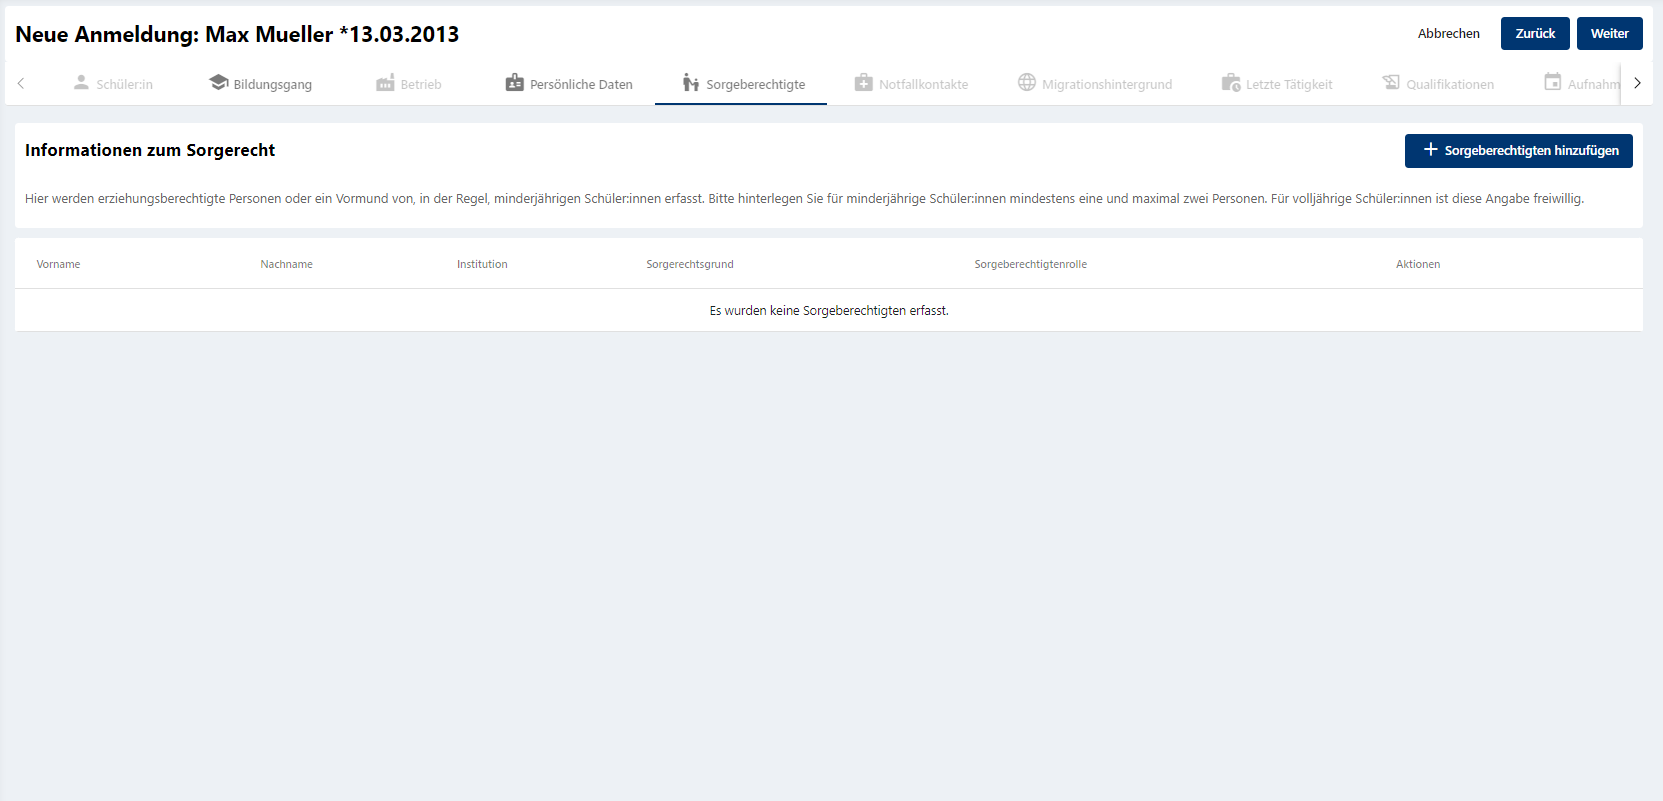
\includegraphics{sorgeberechtigte-liste}
    \end{adjustbox}
\end{figure}

\subsection{sorgeberechtigter-person}
\begin{figure}[H]
    \centering
    \caption{Testüberschrift}
    \begin{adjustbox}{width=0.5\linewidth, center}
        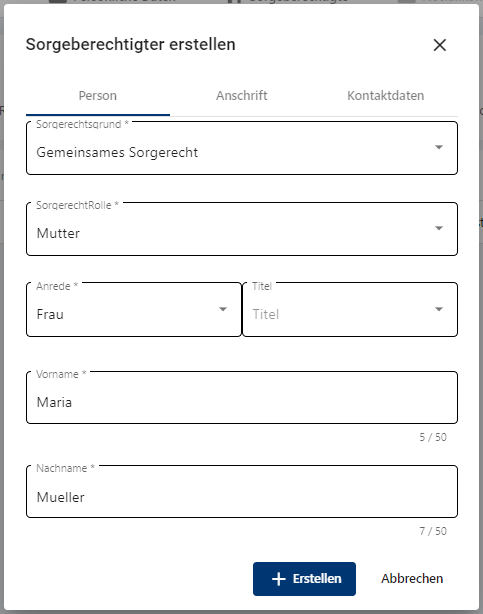
\includegraphics{sorgeberechtigter-person}
    \end{adjustbox}
\end{figure}

\subsection{sorgeberechtigter-anschrift}
\begin{figure}[H]
    \centering
    \caption{Testüberschrift}
    \begin{adjustbox}{width=0.85\linewidth, center}
        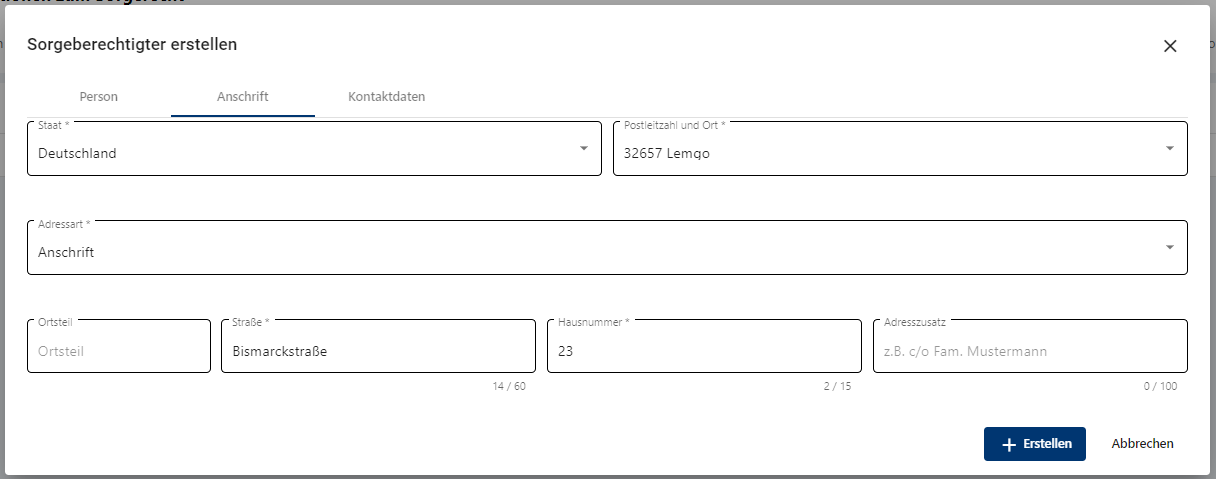
\includegraphics{sorgeberechtigter-anschrift}
    \end{adjustbox}
\end{figure}

\subsection{sorgeberechtigter-kontakt}
\begin{figure}[H]
    \centering
    \caption{Testüberschrift}
    \begin{adjustbox}{width=0.6\linewidth, center}
        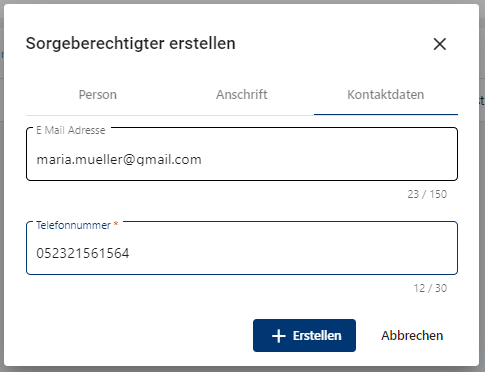
\includegraphics{sorgeberechtigter-kontakt}
    \end{adjustbox}
\end{figure}

\subsection{notfallkontakt-daten}
\begin{figure}[H]
    \centering
    \caption{Testüberschrift}
    \begin{adjustbox}{width=0.6\linewidth, center}
        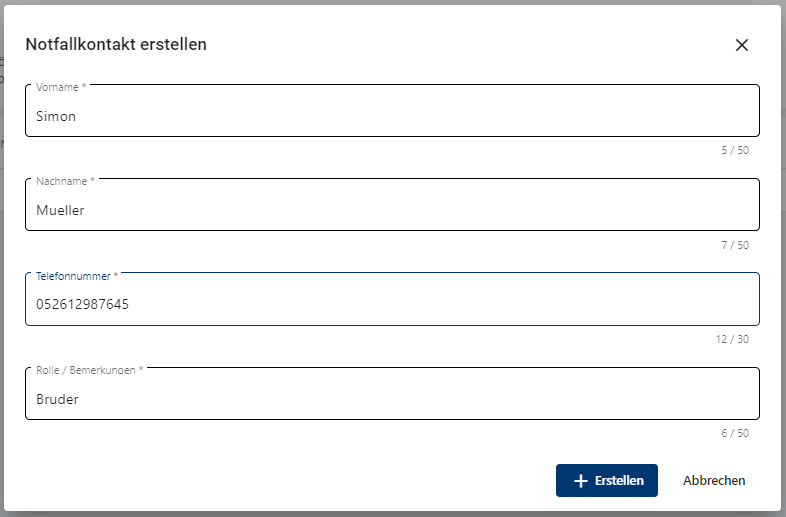
\includegraphics{notfallkontakt-daten}
    \end{adjustbox}
\end{figure}

\subsection{notfallkontakt-liste}
\begin{figure}[H]
    \centering
    \caption{Testüberschrift}
    \begin{adjustbox}{width=\linewidth, center}
        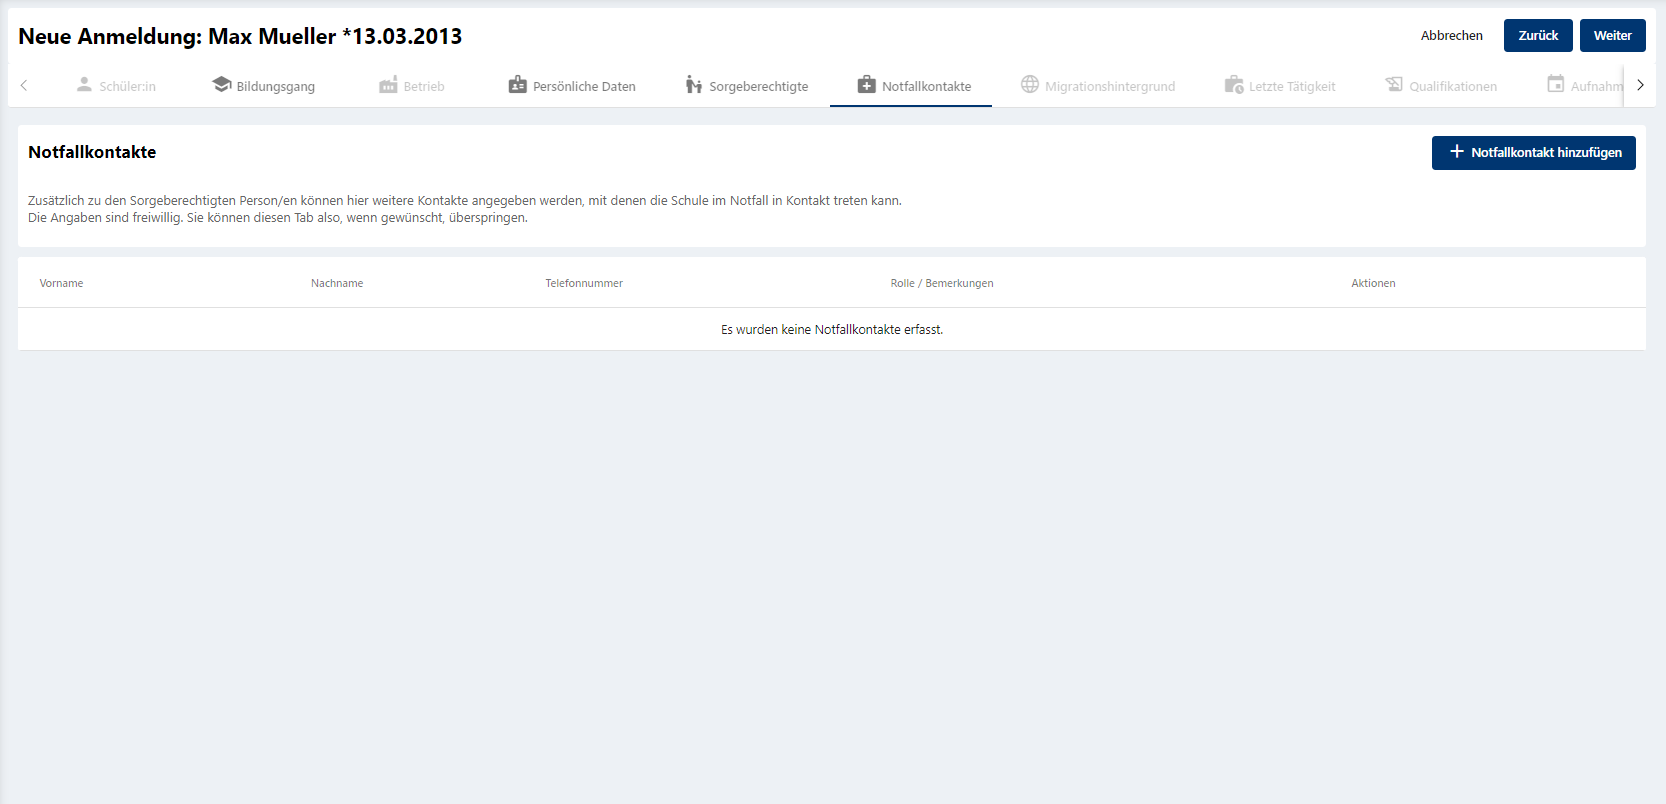
\includegraphics{notfallkontakt-liste}
    \end{adjustbox}
\end{figure}

\subsection{migrationshintergrund-liegtvor}
\begin{figure}[H]
    \centering
    \caption{Testüberschrift}
    \begin{adjustbox}{width=\linewidth, center}
        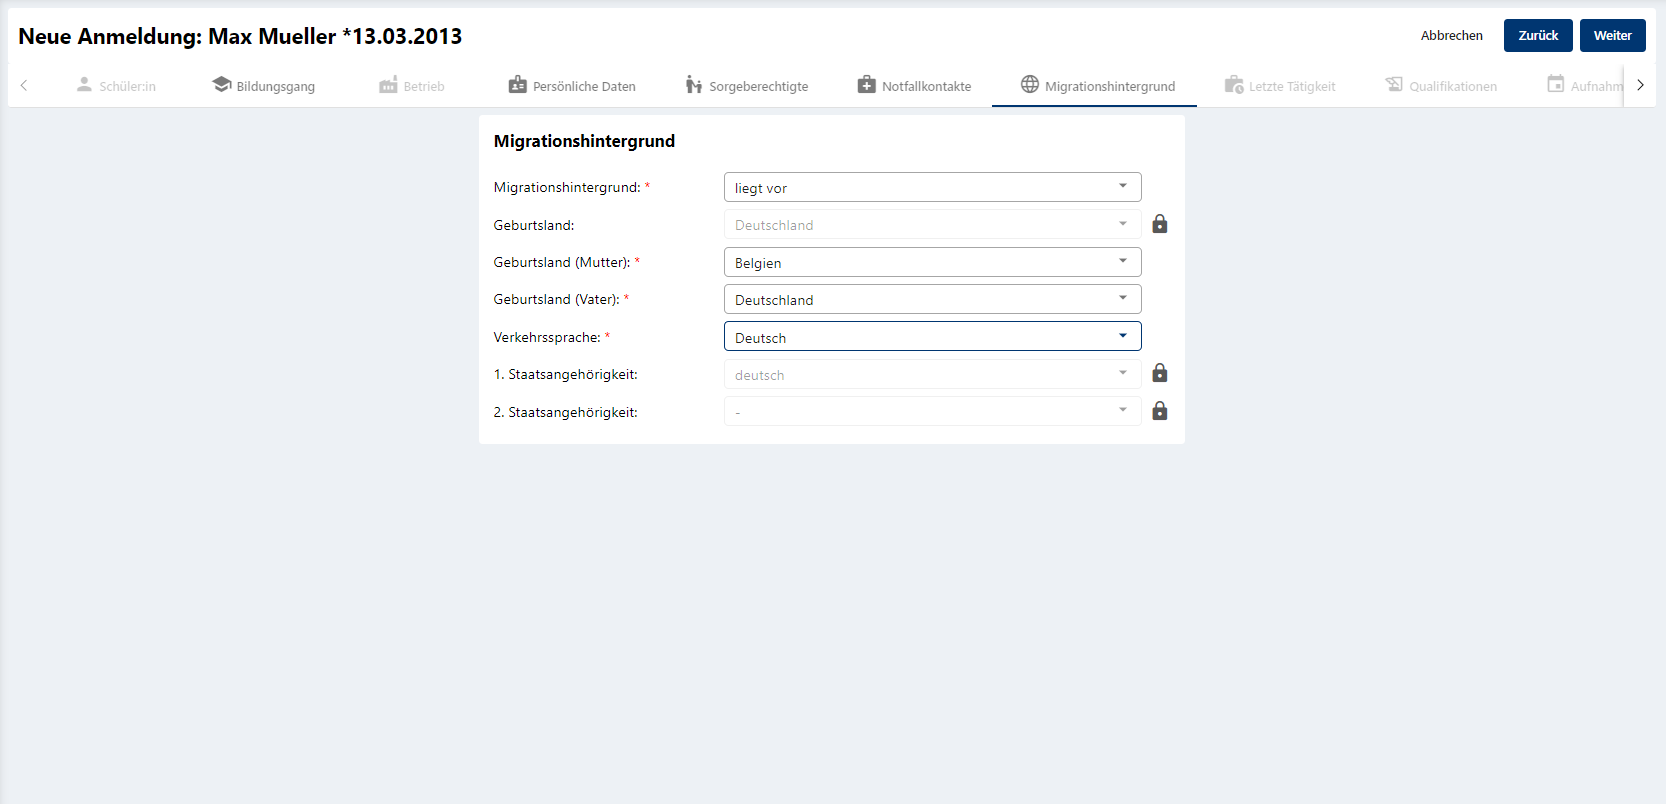
\includegraphics{migrationshintergrund-liegtvor}
    \end{adjustbox}
\end{figure}

\subsection{migrationshintergrund-liegtnichtvor}
\begin{figure}[H]
    \centering
    \caption{Testüberschrift}
    \begin{adjustbox}{width=\linewidth, center}
        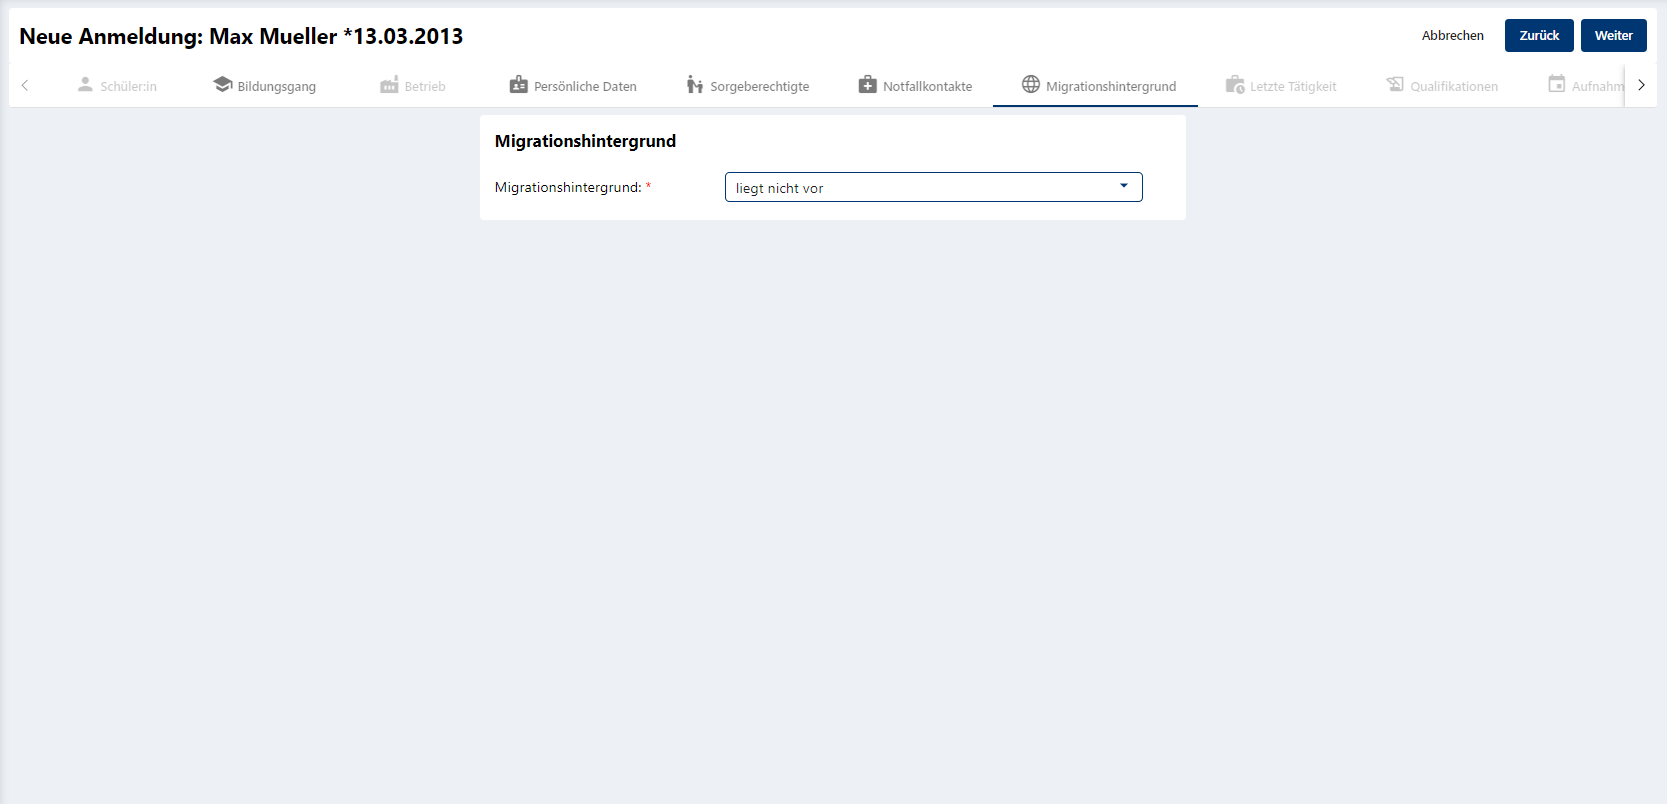
\includegraphics{migrationshintergrund-liegtnichtvor}
    \end{adjustbox}
\end{figure}

\subsection{qualifikation}
\begin{figure}[H]
    \centering
    \caption{Testüberschrift}
    \begin{adjustbox}{width=\linewidth, center}
        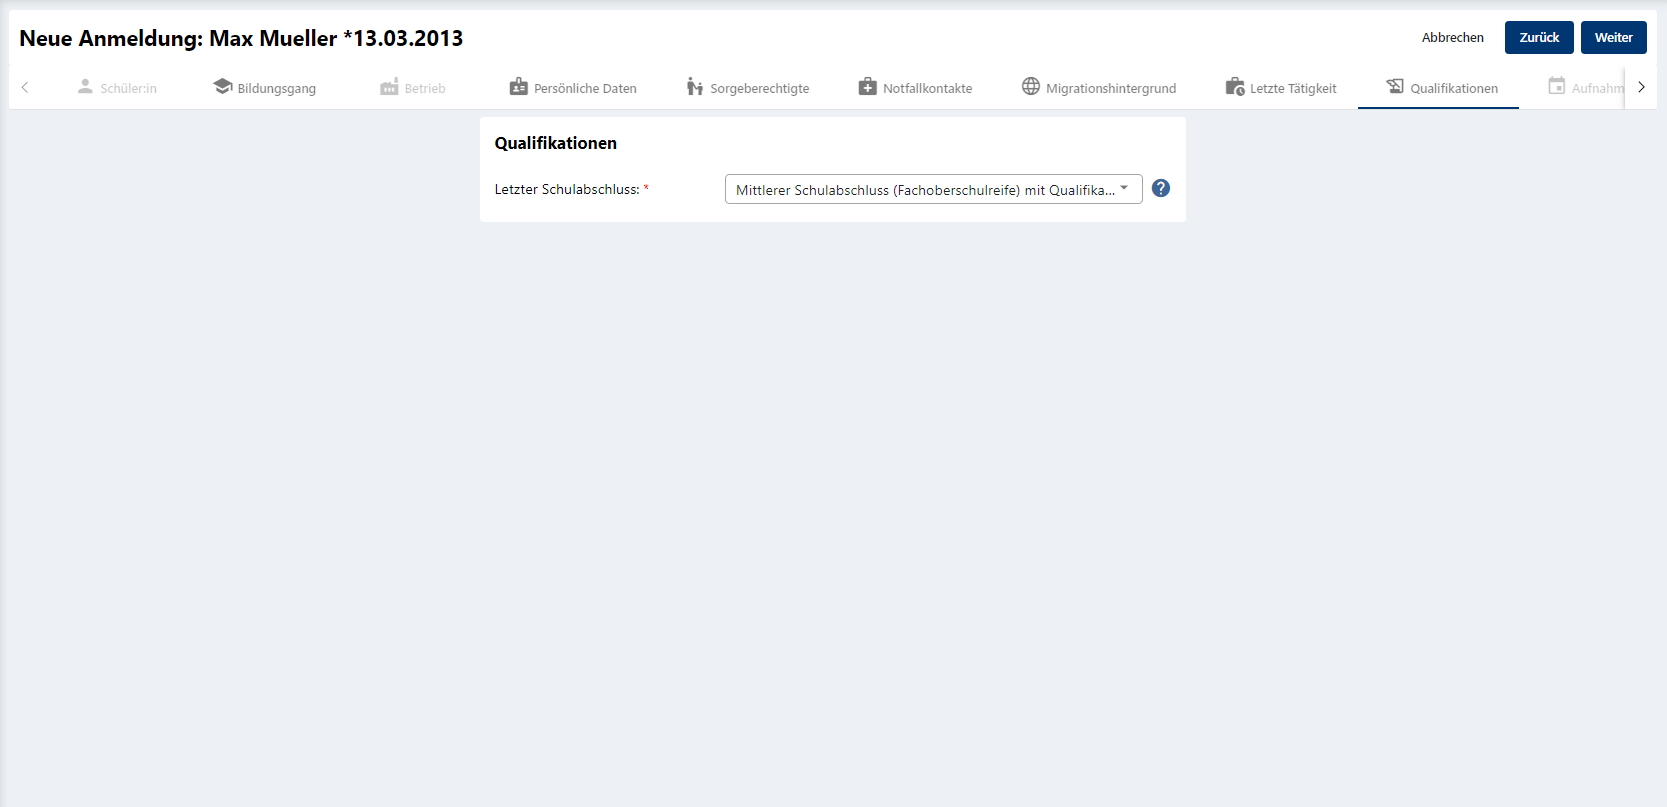
\includegraphics{qualifikation}
    \end{adjustbox}
\end{figure}

\subsection{letztetaetigkeit}
\begin{figure}[H]
    \centering
    \caption{Testüberschrift}
    \begin{adjustbox}{width=\linewidth, center}
        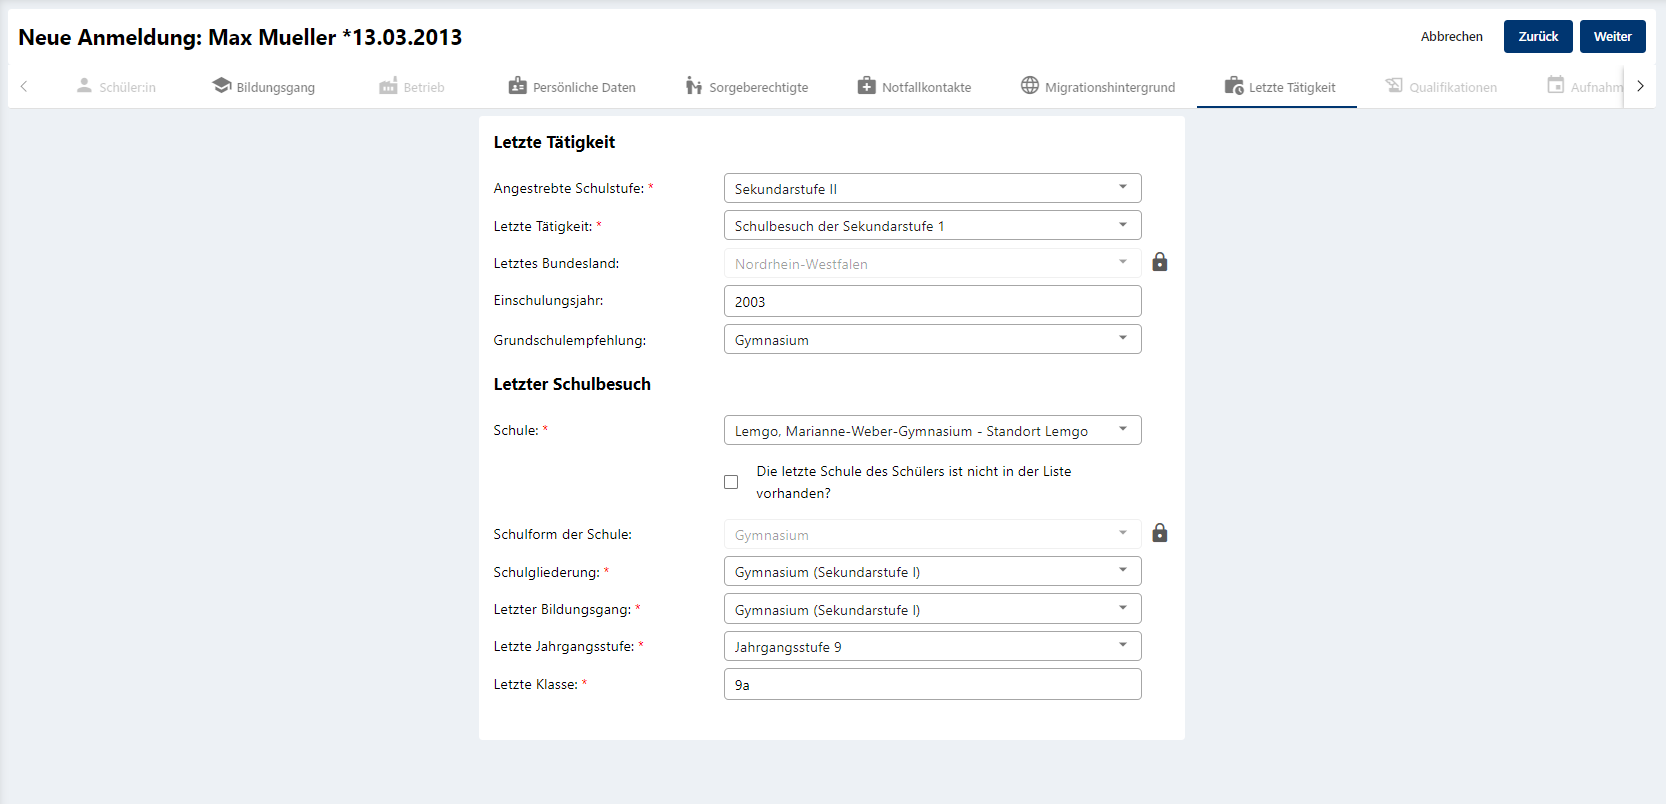
\includegraphics{letztetaetigkeit}
    \end{adjustbox}
\end{figure}

\subsection{aufnahmeberatung}
\begin{figure}[H]
    \centering
    \caption{Testüberschrift}
    \begin{adjustbox}{width=\linewidth, center}
        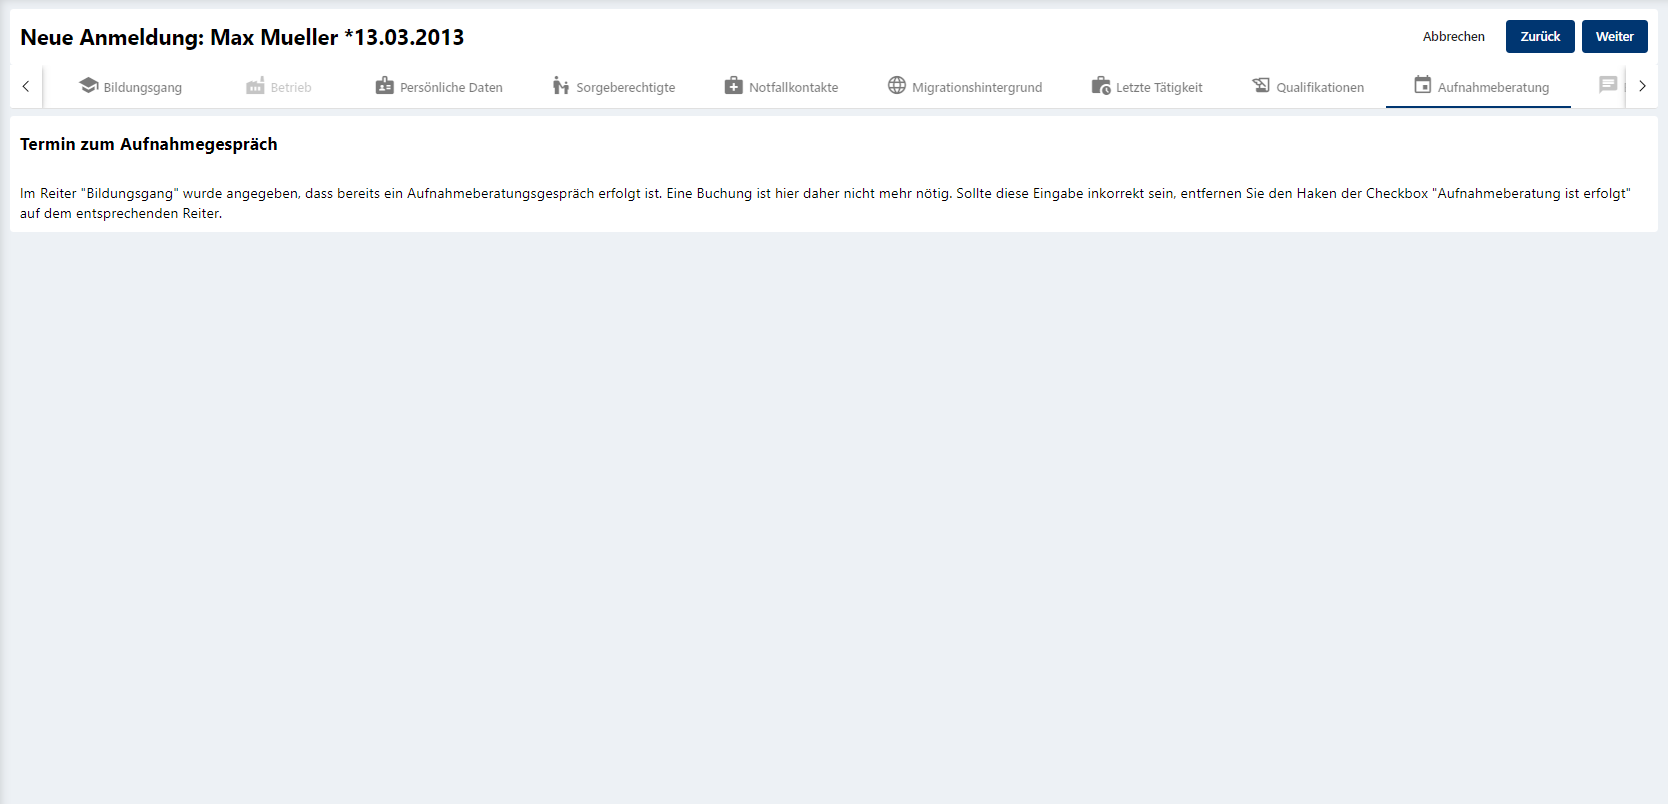
\includegraphics{aufnahmeberatung}
    \end{adjustbox}
\end{figure}

\subsection{bemerkungen}
\begin{figure}[H]
    \centering
    \caption{Testüberschrift}
    \begin{adjustbox}{width=\linewidth, center}
        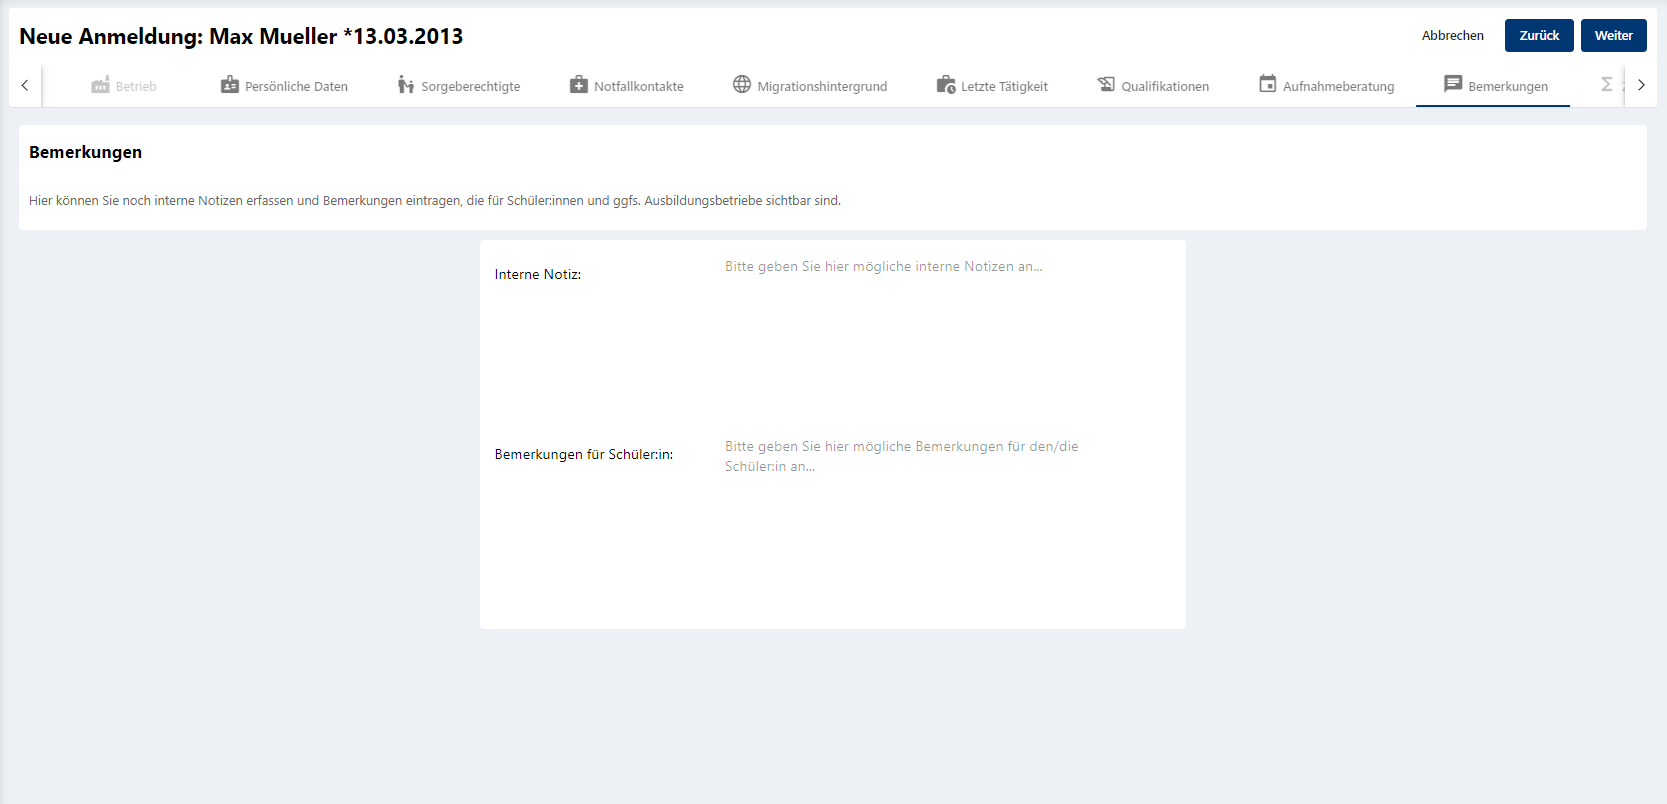
\includegraphics{bemerkungen}
    \end{adjustbox}
\end{figure}

\subsection{zusammenfassung}
\begin{figure}[H]
    \centering
    \caption{Testüberschrift}
    \begin{adjustbox}{width=\linewidth, center}
        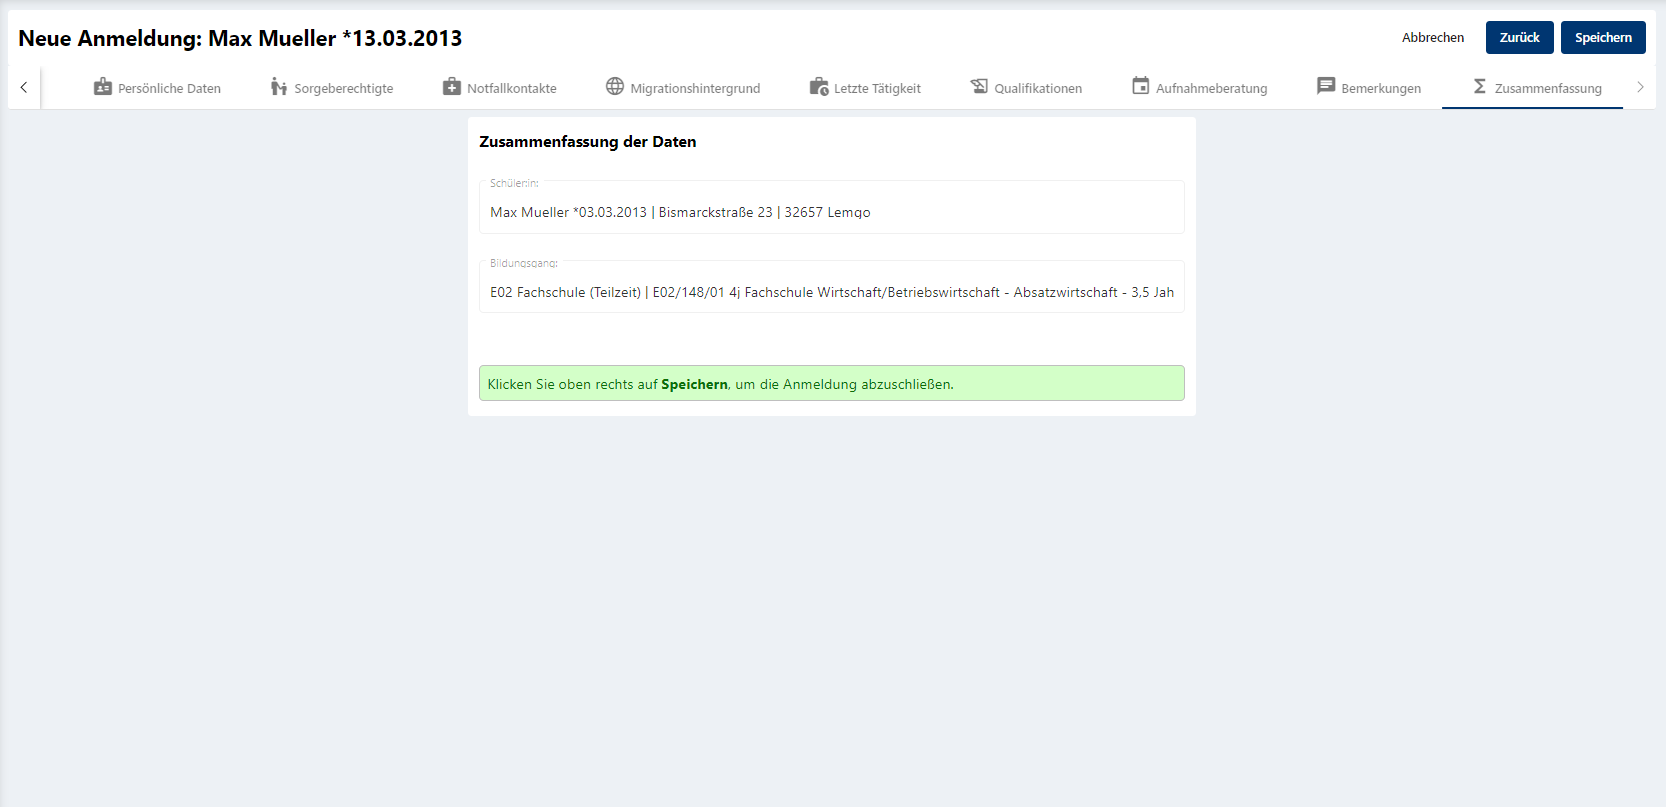
\includegraphics{zusammenfassung}
    \end{adjustbox}
\end{figure}

\subsection{bestaetigung}
\begin{figure}[H]
    \centering
    \caption{Testüberschrift}
    \begin{adjustbox}{width=\linewidth, center}
        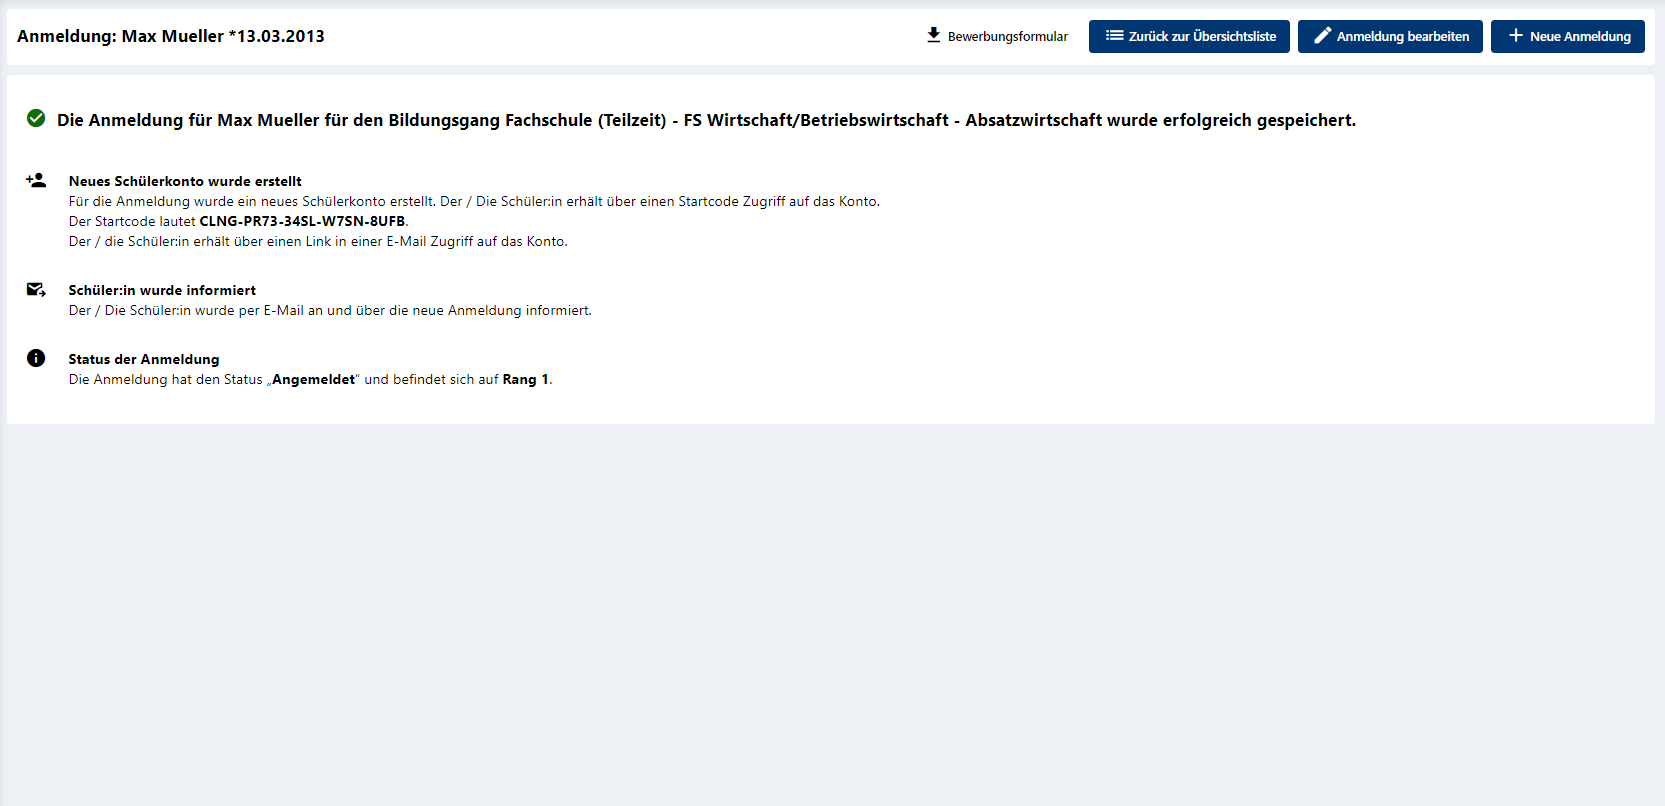
\includegraphics{bestaetigung}
    \end{adjustbox}
\end{figure}

\subsection{update-bewerbung}
\begin{figure}[H]
    \centering
    \caption{Testüberschrift}
    \begin{adjustbox}{width=\linewidth, center}
        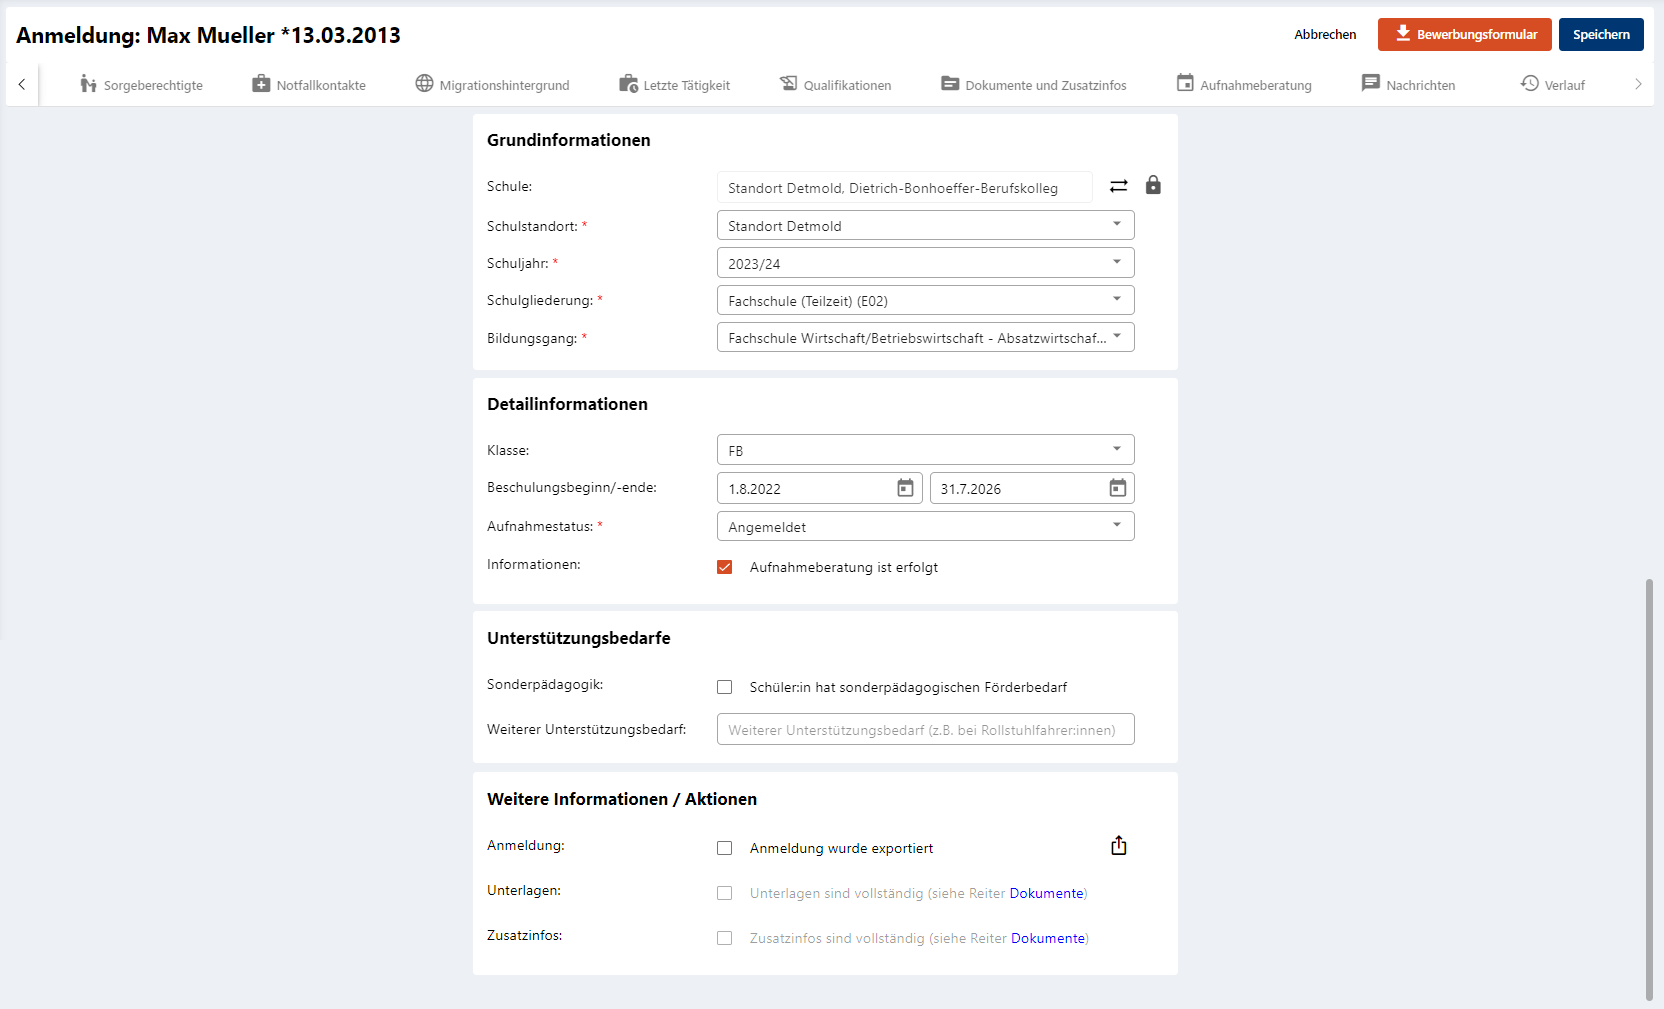
\includegraphics{update-bewerbung}
    \end{adjustbox}
\end{figure}

\end{landscape}


% Bibliographie
\printbibliography

\end{document}
